\documentclass[aps,prd,showpacs,showkeys,notitlepage,preprintnumbers,nofootinbib]{revtex4-1}
\usepackage{amsmath,amssymb,amsthm,bm,color,hyperref,blindtext,fullpage}
\usepackage{graphics,subfigure,rotating,etoolbox,amsbsy,graphicx}
\usepackage[utf8]{inputenc}
\usepackage[toc,page]{appendix}
\usepackage[dvipsnames]{xcolor}
\usepackage{float} %To use H as position
\def\cred{\color{red}}
\def\cgreen{\color{green}}
\newcommand{\todo}[1]{{\cred todo: #1}}
\newcommand{\eq}[1]{Eq.~(\ref{#1})}
\newcommand{\Eq}[1]{Eq.~(\ref{#1})}
\newcommand{\sect}[1]{section~\ref{#1}}
\newcommand{\sects}[1]{sections~\ref{#1}}
\newcommand{\App}[1]{appendix~\ref{#1}}
\newcommand{\fig}[1]{figure~\ref{#1}}
\newcommand{\figs}[1]{figures~\ref{#1}}
\newcommand{\tab}[1]{table~\ref{#1}}
\newcommand{\tabs}[1]{tables~\ref{#1}}
\newcommand{\tr}{\mbox{Tr}}
\newcommand{\nocontentsline}[3]{}
\newcommand{\tocless}[2]{\bgroup\let\addcontentsline=\nocontentsline#1{#2}\egroup}
\setlength{\tabcolsep}{10pt}

\begin{document} 

\title{Neutron electric dipole polarizability}


\author{Michael Engelhardt}
\email{engel@nmsu.edu}
\affiliation{Department of Physics, New Mexico State University,
Las Cruces, NM 88003, USA}
\author{Roman H\"ollwieser}
\email{hoellwieser@uni-wuppertal.de}
\affiliation{Department of Physics, University of Wuppertal,
42119 Wuppertal, Germany}
\affiliation{Department of Physics, New Mexico State University,
Las Cruces, NM 88003, USA}
\author{Jesus Saenz}
\email{jmsaenzv@nmsu.edu}
\affiliation{Institute of Engineering and Technology,
Universidad Aut\'onoma de Ciudad Ju\'arez, 32310, Ciudad Ju\'arez, Mexico}
\affiliation{Department of Physics, New Mexico State University,
Las Cruces, NM 88003, USA}

% \date{\today}

\begin{abstract}
We revisit the neutron electric dipole polarizability and present results from a lattice calculation using the background method with increased statistics, taking into account connected as well as disconnected contributions.  
We further subtract the point-like contribution determined from a Foldy-Wouthuysen transformation in a preceding work. 
\end{abstract}

% \pacs{11.15.Ha, 12.38.Gc}
% not sure we need these anymore

\keywords{Neutron polarizabilities, neutron electric dipole polarizability, lattice QCD}

\maketitle

% \tableofcontents

% \newpage

\section{Introduction}
\label{introsec}
In~\cite{Babusci:1998ww}, the general structure of the cross section in Compton scattering 
with polarized photons and nucleons is discussed. A low-energy expansion
of the scattering amplitudes $T_{if}$ leads to a cross section expression involving
ten nucleon structure parameters, i.e., dipole, quadrupole, dispersion, and
spin polarizabilities. In addition, $|T_{if}|^2$, are written in terms of invariant
amplitudes $T_i$, which are decomposed into Born and non-Born contributions.
Specifically, the spin-independent part of the non-Born contribution to the scattering amplitudes
involve the coefficients $\alpha_E$ and $\beta_M$, i.e., respectively, the
dipole electric and magnetic polarizabilities of the nucleon, which describe
the magnitude of the electric and magnetic dipole moments induced on the nucleon by an
applied electric field $\overrightarrow E$ or magnetic field $\overrightarrow B$\cite{Hagelstein:2020vog}.

 As detailed in~\cite{Detmold:2006vu},the polarizabilities measure the response of the 
 nucleon quark constituents to an applied electromagnetic field. The effective Hamiltonian 
 of the interaction of a nucleon with an external electromagnetic field
is written in terms of ten leading-order terms (in Gaussian units):
\footnote{Polarizability units: In the SI system, there is an additional prefactor of 4$\pi$ and the permittivity $\varepsilon_0$ and permeability $\mu_0$ of the vacuum enter in the corresponding terms in the Hamiltonian.}
\begin{equation}
\begin{split}
H_{\text{eff}^{(2)}}=&-\frac{1}{2}(\alpha_E E^2+\beta_M B^2
+\gamma_{E1}\sigma\cdot\left(E\times \dot E\right)\\
&+\gamma_{M1}\sigma\cdot \left(B\times \dot B\right)
-2\gamma_{E2}E_{ij}\sigma_iB_j+2\gamma_{M2}B_{ij}\sigma_iE_j\\
&+\alpha_{E\nu}\dot E^2+\beta_{M\nu}\dot B^2
+\frac{1}{6}\alpha_{E2}E_{ij}^2+\frac{1}{6}\beta_{M2}B_{ij}^2+\dots)
\end{split}
\label{Heffective}
\end{equation}
where the quadrupole strengths of the electric and magnetic fields are
\begin{equation}
\begin{split}
E_{ij}=&\frac{1}{2}\left(\nabla_iE_j+\nabla_jE_i\right)\\ 
B_{ij}=&\frac{1}{2}\left(\nabla_iB_j+\nabla_jB_i\right)
\end{split}
\end{equation}
and $\alpha_E$ and $\beta_M$ are the electric and magnetic
polarizabilities, $\gamma_{E1}$, $\gamma_{M1}$, $\gamma_{E2}$, and $\gamma_{M2}$ 
are the spin polarizabilities, $\alpha_{E\nu}$, $\beta_{M\nu}$ are the dispersion polarizabilities,
and $\alpha_{E2}$ and $\beta_{M2}$ are the quadrupole polarizabilities~\cite{Babusci:1998ww, Levchuk:1999zy}.
By writing the effective Hamiltonian in the form of~\eq{Heffective}, one assumes a sufficiently
localized nucleon wave function in the sense that its energy depends on the local values of the
electric and magnetic fields and  their derivatives. This matter and the inherent limitations
of~\eq{Heffective} are discussed in more detail in~\cite{Saenz:2020yxy}.

Tripartite efforts are currently underway to determine the nucleon polarizabilities
by experiments, analytically in Chiral Perturbation Theory ($\chi$PT), and by numerical calculation in lattice QCD.

In experimental results, the sum of the electric and magnetic polarizabilities is
an integral of the total photoabsorption cross section in Compton scattering,
i.e., the Baldin sum rule. Additional sum rules and recommended nucleon polarizability values
based on experimental results are presented in~\cite{Schumacher:2019ikn}.
The polarizability addends in the Baldin sum can be singled out by measuring the angular
distribution of the photoabsorption in low-energy Compton scattering~\cite{Hagelstein:2020vog,Levchuk:1999zy}.
For example, in~\cite{Levchuk:1999zy}, deuteron Compton scattering experimental data were fit to
extract the electric and magnetic polarizability of the neutron. An alternative experimental method
is presented in~\cite{Schumacher:2019ikn}, the electric polarizability is measured in the scattering of slow
neutrons in the presence of the electric field of a heavy nucleus, and results for the neutron
polarizabilities are presented as the average of the individual results from deuteron Compton
scattering and neutron electromagnetic scattering by the electric field of a lead nucleus.
Phenomenological extraction of the dipole electric and magnetic, and spin polarizabilities are discussed in~\cite{Holstein:1999uu, Drechsel:2002ar, Hildebrandt:2003fm, Schumacher:2005an, Pasquini:2007hf, Pasquini:2010zr, Griesshammer:2012we, McGovern:2012ew, Holstein:2013kia, COMPTONMAX-lab:2014cve, A2:2014iky, Gryniuk:2015eza, Gryniuk:2016gnm, Hagelstein:2015egb, Griesshammer:2017txw, Pasquini:2017ehj, Pasquini:2018wbl, Pasquini:2019nnx, Miskimen:2019kwu, Martel:2019tgp, A2:2019bqm, Melendez:2020ikd}. Dispersion relation analyses for experimental data of Compton scattering off protons or deuteron at low-energy 
(below pion production or near $\Delta(1232)$ resonance, for example) are discussed to extract nucleon
structure constants such as the polarizabilities.

 Chiral Perturbation Theory, a low-energy effective field theory of the
strong interaction, provides a tool to explore low-energy hadronic physics, such as Compton
Scattering off the nucleon, leading to the calculation of the nucleon electromagnetic polarizabilities
in chiral theory~\cite{Hagelstein:2020vog, Bernard:1991rq, Bernard:1991ru}.

Calculating hadron mass shifts in the presence of external electromagnetic fields in lattice QCD paves a way to calculate nucleon polarizabilities. Some of these efforts are recounted in \cite{Fiebig:1988en, Christensen:2004ca, Lee:2005dq, Shintani:2006xr, Engelhardt:2007ub, Engelhardt:2009ryp, Detmold:2009dx, Detmold:2010ts, Engelhardt:2011qq, Alexandru:2009id, Lee:2010dq, Lee:2011gz, Lujan:2014kia, Freeman:2014kka, Luschevskaya:2014lga, Lujan:2016ffj, Primer:2013pva, Bignell:2018acn, Bignell:2020xkf, Bignell:2020dze, He:2020ysm, Bignell:2020aye}.
Measurements on the lattice are performed on finite volumes and at unphysical (heavy) pion masses. The polarizabilities are given by the neutron mass shift in the presence of external static electric and 
magnetic fields, precisely on the part of the mass shift that is quadratic-in-the-fields. Chiral effective
theory aims to connect lattice results to the pion mass and infinite volume physical limits~\cite{Detmold:2006vu, He:2020ysm, Hildebrandt:2003fm, Lensky:2015awa, Griesshammer:2015ahu}. As mentioned, the polarizability coefficients in~\eq{Heffective} can be 
connected to the Compton scattering amplitudes in the low-energy limits. Matching the background field
calculations of the polarizabilities in lattice QCD to the effective field theory description of the Compton
amplitudes is explored amply in~\cite{Lee:2013lxa, Lee:2014iha}, for example.

In this work, we focus on the lattice measurements of the electric polarizability $\alpha_E$ of the neutron.
While other works on lattice hadron polarizability measurements have been performed in the quenched approximation~\cite{Fiebig:1988en, Wilcox:1996vx, Wilcox:1997ee, Zhou:2002km, Christensen:2002wh, Christensen:2004ca, Lee:2005dq, Lee:2005vv}, in this work, we use a dynamical quark ensemble with a pion mass of 357 MeV, and improve the measurements of the electric polarizability of the neutron as compared to those reported in~\cite{Engelhardt:2007ub, Engelhardt:2009ryp} by considering connected and disconnected diagram contributions. In future work, we will present the lattice measurement of the spin electric polarizability $\gamma_{E1}$.



\section{Calculation method}
This work improves the results of the neutron electric polarizability, which is obtained by the extraction of the hadron mass from the neutron two-point function in the presence of an external static electric field. The method has been applied successfully in~\cite{Engelhardt:2007ub, Engelhardt:2009ryp},
but our work improves the neutron electric polarizability lattice measurements
threefold; firstly, this work uses data sets with improved statistics, as compared to the previous calculations efforts in~\cite{Engelhardt:2007ub, Engelhardt:2009ryp}. Secondly, point neutron sinks are used. The former improvement
 in the data sets yield better statistical uncertainty in the correlators, while the latter
 avoids additional time dependencies related to smeared neutron sinks, which are discussed below
 and in~\cite{Engelhardt:2007ub}. Thirdly, the point-like contribution to the 
 electric polarizability has been accounted for, i.e., the Foldy contribution, 
 as presented in~\cite{Saenz:2020yxy}, has been subtracted from the lattice measurements, 
 yielding a \textit{bona fide} neutron polarizability.
 
The neutron two point function is the correlator
\begin{equation}
\langle N_{\beta}(y)\overline N_{\alpha}(x)\rangle= \frac{1}{Z}\int[DU][D\overline \psi][D\psi]
\exp(-S[\psi,\overline \psi, U])N_{\beta}(y)\overline N_{\alpha}(x)
\label{correlator}
\end{equation}
where the action $S$, and the neutron fields $N, \overline N$ depend on the external
electromagnetic field. After decomposing the action into one with vanishing external field
plus one with the electromagnetic perturbation, i.e., $S=S_0+S_E$, the correlator in
\eq{correlator} can be written in the form
\begin{equation}
\langle N_{\beta}(y)\overline N_{\alpha}(x)\rangle=\frac{\langle e^{-S_E}N_{\beta}(y)\overline N_{\alpha}(x)\rangle_0}
{\langle e^{-S_E}\rangle_0}
\end{equation}
that is, in terms of the averages in the absence of the external field.
As mentioned in~\sect{introsec}, the electric polarizability can be extracted from
the quadratic-in-the-field part of the neutron mass. This translates to finding the
aforementioned quadratic term in the Taylor expansion with respect to the applied
electric field. The neutron two-point function becomes
\begin{equation}
\langle N_{\beta}(y)\overline N_{\alpha}(x)\rangle=
\frac{\int[DU][D\psi][D\overline \psi]\exp(-S_0)(1-S_E+S_E^2/2+\dots)N_{\beta}(y)\overline N_{\alpha}(x)}{\int [DU][D\psi][D\overline \psi]\exp(-S_0)(1-S_E+S_E^2/2+\dots)}
\end{equation}
The external electric field is taken in this work to point in the 3-direction, as 
described by~\eq{gauge}, i.e., the gauge field is non-zero and linear in the electric field.
In such a case, the external electric field modifies the gauge links as
\begin{equation}
U_3\rightarrow\exp\left(iq\int dx_3\cdot A_3\right)\cdot U_3=(1+iaqA_3-a^2q^2A_3^2/2+\dots)\cdot U_3
\label{gaugelink}
\end{equation}
where $a$ is the lattice spacing and where $q$ the quark fractional electric charge
according to flavor. As explained in~\cite{Engelhardt:2009ryp}, after inserting \eq{gaugelink} into
the fermion action discretization of the Wilson type, two interaction vertices emerge, one
linear in the external electric field while the other is quadratic; the coupling to the
external electric field becomes
\begin{equation}
\begin{split}
S_E=z_v\frac{1}{2}\sum_x \overline{\psi}(x)((&iaqA_3-a^2q^2A_3^2/2)\cdot U_3(x)\cdot
(-1+\gamma_3)\cdot \psi(x+e_3)\\
&+(iaqA_3-a^2q^2A_3^2/2)\cdot U_3^\dagger(x-e_3)\cdot(1+\gamma_3)\cdot\psi(x-e_3))
\end{split}
\label{interaction}
\end{equation}
where $z_v$ is a renormalization factor that compensates the renormalization of the
vertices in \fig{fig:diagrams}. The quark lines in these diagrams are populated
by four-dimensional domain wall fields, and the coupling of said quark lines to the
external field is attained via the current obtained from projecting the quark modes $\overline \psi$,
$\psi$ onto the domain walls~\cite{Engelhardt:2009ryp}.
As explained in~\cite{Engelhardt:2007ub}, Wick's theorem yields the diagrammatic 
representation (c.f. figure~\ref{fig:diagrams}) of the quadratic term in the Taylor expansion, 
with respect to the applied electric field, of the neutron two-point function.
\begin{figure}[h!]
  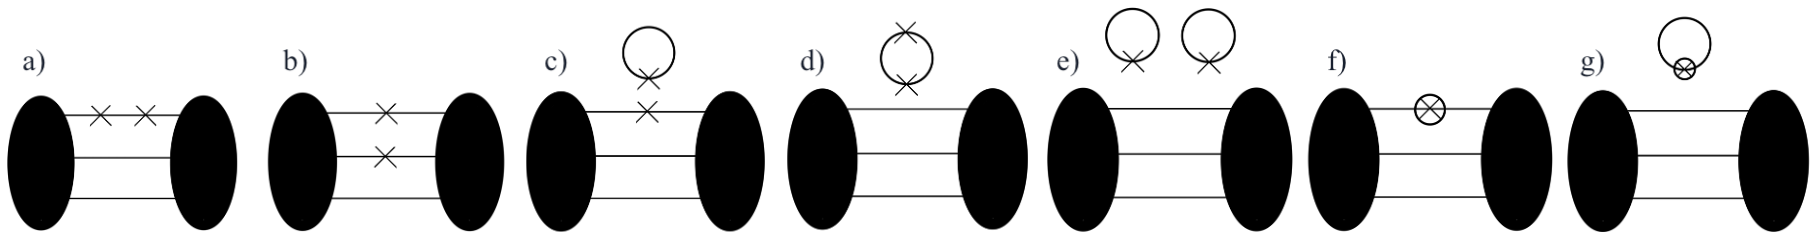
\includegraphics[width=15cm]{figures/diagrams.png}
  \caption{Relevant diagram contributions to the neutron electric polarizability. Note that the 
  crosses indicate the interaction vertices; linear in the external field interactions are represented with crosses, while the quadratic in the field interaction are represented by circles.}
  \label{fig:diagrams}
\end{figure}
In the case of a time-independent Hamiltonian that depends on the electric field
$E$ and gauge field $A$, which are considered to be two arbitrarily small parameters,
projecting onto unpolarized, zero-momentum neutrons, the two-point function
exhibits an exponential behavior at a large time:
\begin{equation}
G(p=0,t)=\sum_{\overrightarrow y}Tr\left(\frac{1+\gamma_0}{2}\langle N(y)\overline N(x)\rangle\right)\
\overset{t\rightarrow \infty}{\longrightarrow} W\exp(-mt)
\end{equation}
Expanding in $A$ and $E$, the overlap between the neutron source and the
ground state $W$, and the neutron mass $m$ are written as
\begin{equation}
\begin{split}
W&=W_0+W^{(1)}(A,E)+W^{(2)}(A,E)+\cdots\\
m&=m_0+m^{(2)}(A,E)+\cdots
\end{split}
\end{equation}
The second-order term in $A$ and $E$ in the neutron two-point function
is written as
\begin{equation}
G^{(2)}(p=0,t)\overset{t\rightarrow \infty}{\longrightarrow}W_0\exp(-m_0t)\left(\frac{W^{(2)}(A,E)}{W_0}-m^{(2)(A,E)t}\right)
\end{equation}
and, thus, the neutron mass shift $m^{(2)}$ can be obtained from the temporal slope of the 
correlator ratio, defined as
\begin{equation}
R_2(t)=\frac{G^{(2)}(p=0,t)}{G^{(0)}(p=0,t)}
\label{ratios}
\end{equation}


\section{Measurement Results}
\subsection{Quark renormalization}
As discussed already in~\cite{Engelhardt:2007ub, Engelhardt:2009ryp}, we need to renormalize our results. The renormalization factor $z_v=3/Q$, where $Q$ is a measurement of the number of valence quarks in the neutron, is
deduced by measuring the three-point function without weighting by the quark electric charge $q_f$ in the presence of an external gauge field of the form 
\begin{equation}
A_o=\delta(x_0-t)
\end{equation}
for some time $t$ between the hadron source and sink. The lattice regularization makes
the number $Q=\int d^3xj_o$ deviate from 3, where $j_0$ is the temporal component of the 
quark current. One can obtain the number of quarks by averaging
measurements of $t$ at different lattice times. In this work, these measurements
where taken at insertion times $t$ in the interval $4a\le t \le8a$, while 
the sink is introduced at $t_{\text{sink}}=13a$. The uncertainties in both $Q$ and
$z_v=3/Q$ were obtained by the jackknife method. As remarked in~\cite{Engelhardt:2009ryp},
light and strange quark lattice currents have different renormalization factors.
To measure the aforementioned renormalization factors, the ratios $Q_l, Q_s$,
respectively light and strange quarks, of the data with
and without insertion should reach plateau values. The renormalization factors are then
$3/Q_l$ and $3/Q_s$. Taking into account all diagrams in \fig{fig:diagrams}, every connected insertion is 
renormalized by the first value, but either renormalizes every loop insertion, e.g.,
a connected plus strange loop, or a mixed light-strange loop, is renormalized by a factor $9(Q_lQ_s)$.
The charge renormalization factors for light and strange quarks on the $m_{\pi}=357$ MeV ensemble were measured to be
\begin{align}
Q_l=2.629(20)&\Rightarrow z_{v,l}=1.1412(86)\\
Q_s=2.7354(22)&\Rightarrow z_{v,s}=1.09671(89)
\end{align}
\subsection{Foldy-Wouthuysen contribution to $\alpha_E$ at $m_\pi$= 357 MeV.}
In order to extract the lattice measurement of the neutron's electric polarizability,
one has to calculate the point-like contribution present in its energy spectrum. Such a 
a contribution to dipole electric polarizability in long-know~\cite{Foldy:1959zza}. There are ten
leading Foldy contributions for a zero-momentum neutron, which were determined
from a Foldy-Wouthuysen transformation constructed in such a form as to yield
the energy shift of a neutron in the presence of an external electromagnetic field.
These contributions are reported in~\cite{Saenz:2020yxy}, and the Foldy-Wouthuysen
electric polarizability contribution $\alpha_{\text{FW}}$ is
\begin{equation}
\alpha_{\text{FW}}=\frac{-\mu^2}{m_n}
\label{fwcontrib}
\end{equation}
where $\mu$ is the anomalous magnetic moment of the neutron and $m_n$ is the 
neutron mass. Given that the lattice measurements of the electric polarizability are
conducted at $m_\pi=$ 357 MeV, the point-like contribution in \eq{fwcontrib} has to be
evaluated at the pion mass scale. In~\cite{Green:2019zhh}, the isovector and
isoscalar normalized anomalous magnetic moments are given by 
$\kappa_v^{\text{norm}}=2.518(57)$ and $\kappa_s^{\text{norm}}=-0.030(22)$
in magnetons\footnote{Note, in this work a pion mass of $m_\pi=$ 355 MeV was given, which however corresponds to the same ensemble as the present one.}. 
The neutron anomalous magnetic moment is given by
\begin{equation}
\kappa=\frac{\kappa_s^{\text{norm}}-\kappa_v^{\text{norm}}}{2}=-1.274(31)
\end{equation}
As a function of the neutron mass $m_n$, the magnetic moment in GeV$^{-1}$ is
\begin{equation}
\mu=\kappa\sqrt{\frac{1}{137}}\frac{1}{2m_n^{\text{phys}}}
\label{anomalous}
\end{equation}
Evaluating~\ref{anomalous} at the physical neutron mass $m_n^{\text{phys}}$, as given 
in~\cite{ParticleDataGroup:2016lqr}, the magnetic moment is then
\begin{equation}
\mu_{357\text{ MeV}}=-0.0579(14)\text{ GeV}^{-1}
\label{magmom}
\end{equation}
On the other hand, at $m_\pi=355.98(80)$ MeV the {\cred neutron mass is $m_n=1154.8(80)$???} 
MeV, as given in~\cite{LHPC:2010jcs}. This mass value, along with the result given in~\ref{magmom}, lead to 
a Foldy-Wouthuysen contribution (c.f.~\ref{fwcontrib})
\begin{equation}
\alpha_{\text{FW}}^{357\text{ MeV}}=(-0.2232\pm7.7\times 10^{-7})\text{ }10^{-4}\text{ fm}^{-3} {\cred error???}
\end{equation}
As detailed in~\cite{Saenz:2020yxy},~\eq{fwcontrib} results from the energy shift of a 
poin-tlike neutron, so it must be subtracted from the $\alpha_E$ obtained from the lattice 
measurements described in this work.
%%%%%%%%%%%%%%%%%%%%%%%%%%%

\subsection{Neutron mass shift}
\subsubsection{Numerical measurements}

The numerical results discussed in this work are the result of the analysis of 448 gauge configurations generated with dynamical asqtad staggered quarks~\cite{Lepage:1998vj}, provided by the MILC collaboration~\cite{Bernard:2001av}. The lattice spacing $a =$ 0.124 fm, with bare quark
masses $am_l$ = 0.01 and $am_s$ = 0.05, which corresponds to a pion mass of 357 MeV. 
The quark lines of the diagrams in \fig{fig:diagrams} that contribute to the neutron electric polarizability were
populated with domain wall quarks, the disconnected contributions were estimated using complex $Z(2)$ stochastic sources. A technicality has been identified in~\cite{Engelhardt:2007ub}: a time-independent Hamiltonian ensures a stationary neutron wave function, while a time dependence is introduced by smeared neutron sinks, which would have to be addressed by considering additional contributions from additional diagrams to those shown in \fig{fig:diagrams}. In order to avoid these systematic effects we use point-like neutron sinks  which are time-independent and invariant under gauge transformations of the external field. After first measurements we found the denominator of the correlator ratio $R_2(t)$ in \eq{ratios} to be quite noisy, and therefore improved its statistics. For the results including disconnected diagrams in particular, the improved statistics however did not pay off and therefore we also quote the results of the original measurements.  

\todo{describe electric field and 1 vs. 3 window fits...

A constant electric field is introduced in the 3-direction of the gauge field of the form
\begin{equation}
A_3=E(t-t_0).
\label{gauge}
\end{equation}
Different choices of time $t_0$ correspond to time shifts of the gauge component. Measurements at different $t_0$ allow one to treat
the finite lattice effects, as the neutron energy spectrum depends on the gauge field $A$.
It has been shown that there is a strong dependence of the nucleon polarizabilities on
lattice volume, and it is claimed that a correction below 10\% can be made. The finite volume corrections are
found by studying the volume dependence of the values of polarizability obtained in calculations performed
on lattices of different size~\cite{Lujan:2016ffj}.
The constant gauge field dominant effect is further elaborated in~\cite{Engelhardt:2007ub}. Furthermore, 
the present work used only one spatial lattice volume. Thus, to treat finite-size effects, polarizability
measurements were performed at three different time values corresponding to three constant shifts of $A_3$.
The polarizability measurements where made at $t_0=-10a,\ 0,\ 6a$. These choices correspond 
to the three-window analysis, which probes the behavior of the correlation ratio $R_2$ at three times, 
thus defining the parabola of temporal slopes of the correlator ratio. In turn, the extremal slope
corresponds, with a minus sign, to the mass shift of the neutron at the stationary point. In our work,
the extremal slope was corrected for curvature effects; the need for such a correction arises
from our fitting of linear functions, for a selected range of data points, to the cubic behavior
of the correlator ratio, as will be discussed shortly.

The generic behavior of the correlator ratios in \eq{ratios} is cubic as a function of time steps $t/a$.
In our 3-window analysis, three values of the slope are obtained from a selected range of different 
data sets. These three slope values correspond to three points in a quadratic function, a parabola that
results from the derivative of the cubic function that represents the generic behavior of the correlator
ratios. Note that in each time window, a range of data has to be selected to obtain from it the slope.
In our work, linear functions were fitted to the ranges of each of the data sets. This procedure yields
slope, or points in a parabola, whose values deviate from the true values obtained from a
cubic function. To define the correction to the minima, we defined a range $M$ of data points,
which is the difference between the final and initial time steps in the range. Assuming that a cubic
function describes a set of perfect data points, we considered the sum of the squares of said
perfect data point in a cubic function. By minimizing the sum, in turn, with respect to the slope
$p$ of the linear term and with respect to the constant term $q$ of the linear function, an expression
for $p$ in terms of $M$ and of the coefficients of the cubic function was obtained. The form of
$p$ is quadratic in time step $s$, say. The three values on the parabola
were taken as the values of the slope at $s$= 21,11, 5. On the other hand, the exact minimum
of a parabola is obtained in a straightforward calculation, starting from a function quadratic in time 
step $t$. By comparing the forms of the quadratic in $s$ and quadratic in $t$ functions, a correction
$\Delta p$ for the minimum of the parabola was found. Said correction has an interesting and useful
feature; it is a constant that depends on the fitting range $M$. This means that the same correction 
may be applied to any and all time windows. The correction of the extremum was applied 
to the extracted minima of the fitted quadratic function.

The slopes presented in this work were obtained by performing $\chi^2$ 
fits to the $R_2(t)$ data for a range of choice $5a\le t\le7a$ in the three-window analysis,
in which linear functions are fitted for the selected range at the three time windows
of the cubic correlator ratio. As mentioned, the slopes obtained from these fits are three points in
a quadratic function, which represents the derivative of the cubic function, for which the
extremal value is determined. These extremal values were corrected for curvature of the
fitted function, as justified above. This work also considers the fitting ranges $4a\le t\le 8a$ and $3a\le t\le 9a$ 
as alternatives. 
}


%%%%%%%%%%%%%%%%%%%%%%%%%%%
\subsubsection{Electric polarizability $\alpha_E$ from connected diagrams in the 3-window analysis}
\label{357}
 
 The static electric polarizability for the three fitting ranges are presented 
 in~\tab{tab:ConnectedPolarizabilities} with and without the Foldy-Wouthuysen contribution~\cite{Saenz:2020yxy}. 
 The electric polarizability measurements are consistent with those reported in~\cite{Engelhardt:2009ryp}. 
 
\begin{table}[H]
\begin{center}
    \begin{tabular}{|l|l|l|l|}
    \hline
     Fit range $[t/a]$ 		& 5 to 7   	& 4 to 8   	& 3 to 9  	\\ \hline
     Inflection point $[t/a]$ 	& 6.43(24)& 6.7419) 	& 7.28(13) \\ 
     					& 6.27(27)	& 6.59(20)	& 7.15(14) \\ \hline
     Extremal slope $[a^3]$ & -0.0127(77) 	& -0.0149(58) 	& -0.0194(42) \\ 
     					& -0.0151(78) 	& -0.0154(59) 	& -0.0185(43) \\ \hline
    \end{tabular}
\end{center}
\caption{Inflection points and extremal slopes of the $\chi^2$ linear fits in the 3-window analysis with parabola minimum lift \textcolor{red}{correction} for connected diagrams. \todo{results from reduced statistics are given in the lower lines}}
\label{Table:ConnectedMultipoint}
\end{table}


\begin{figure}[H]
\centering
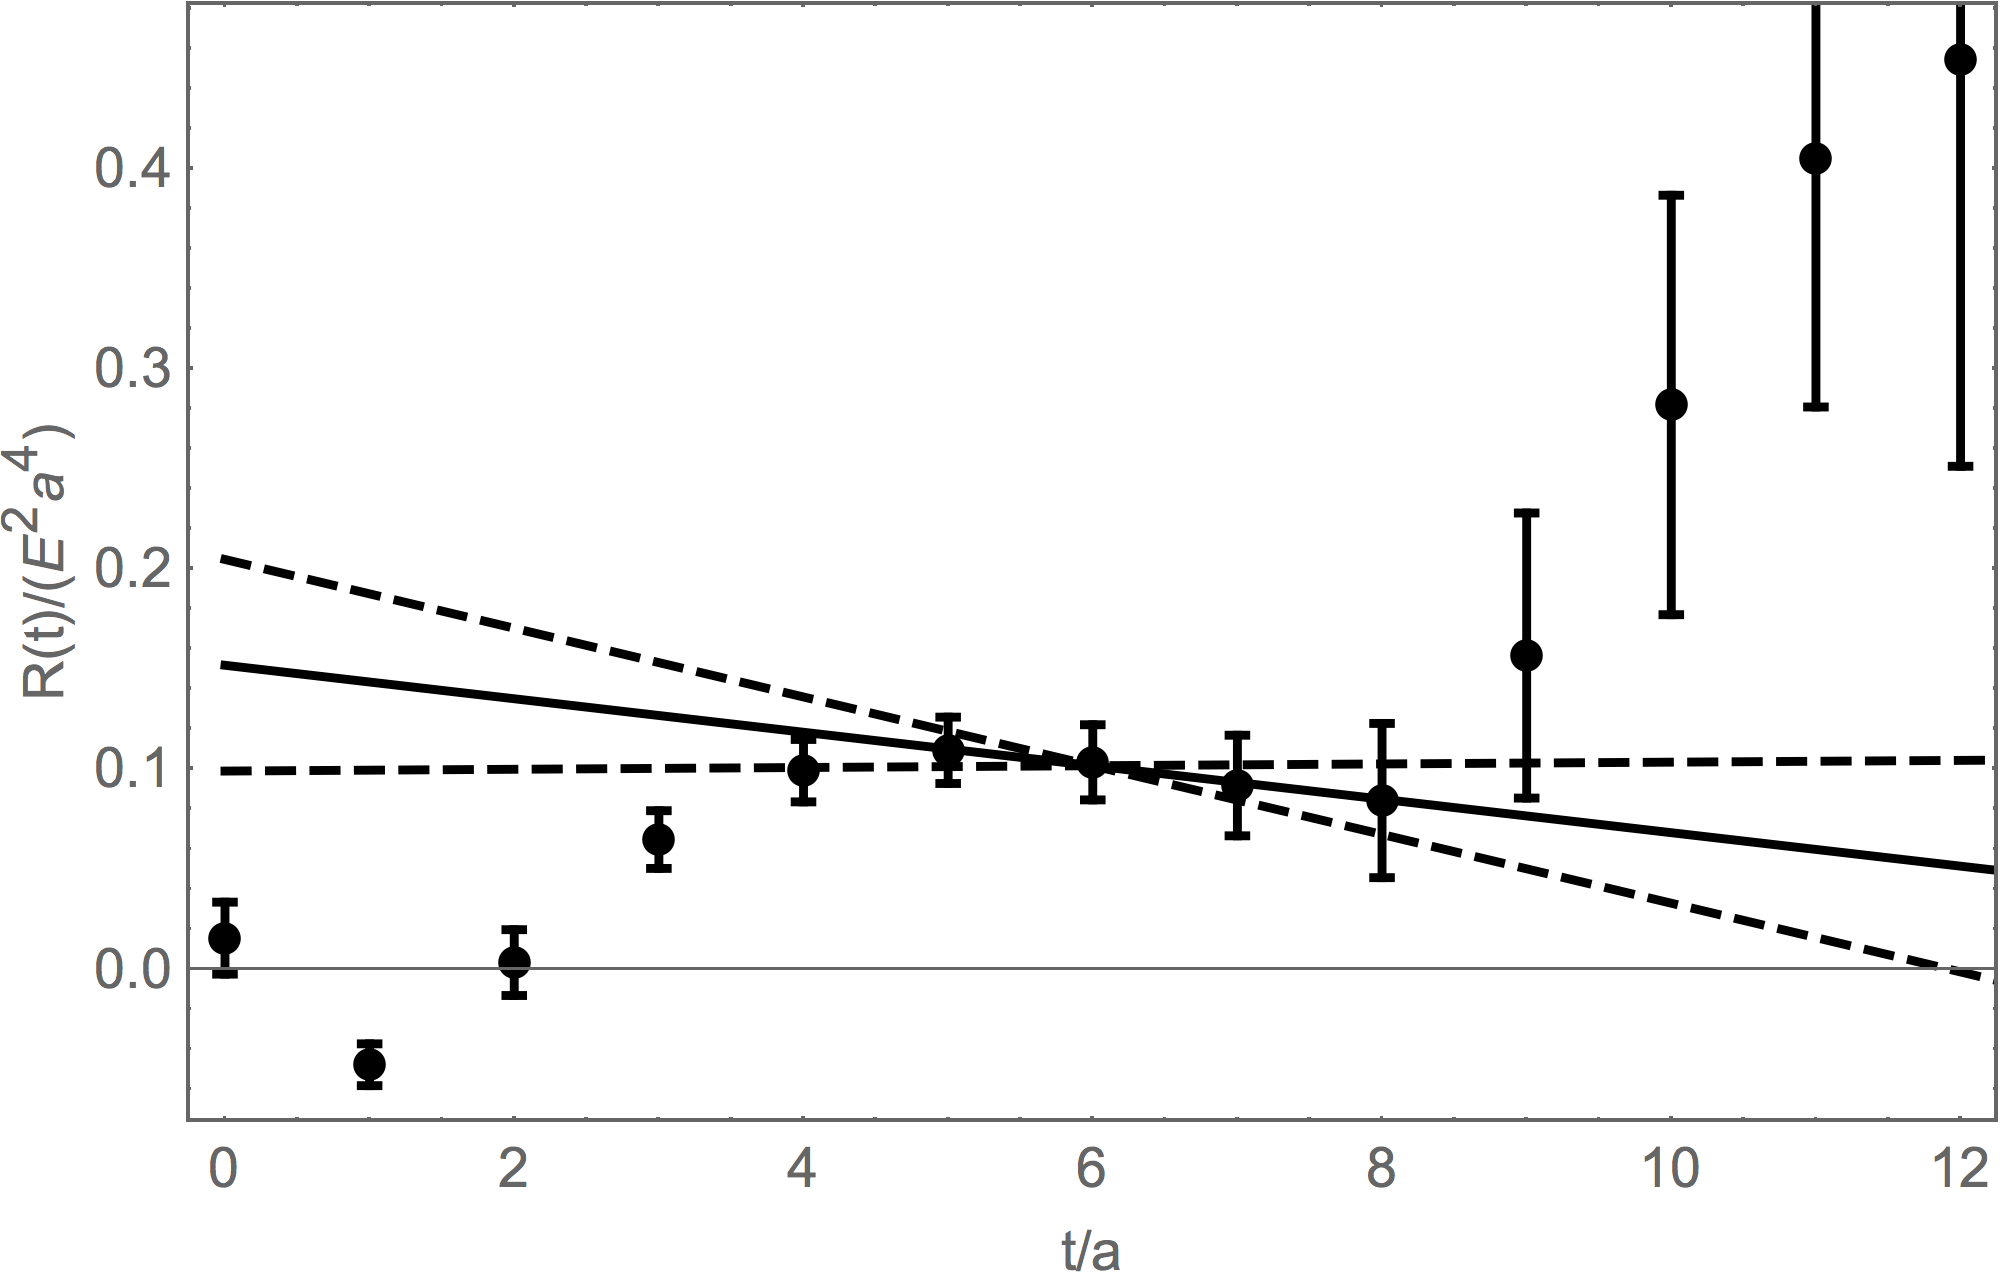
\includegraphics[width=.33\linewidth]{figures/shshLineCS.png}
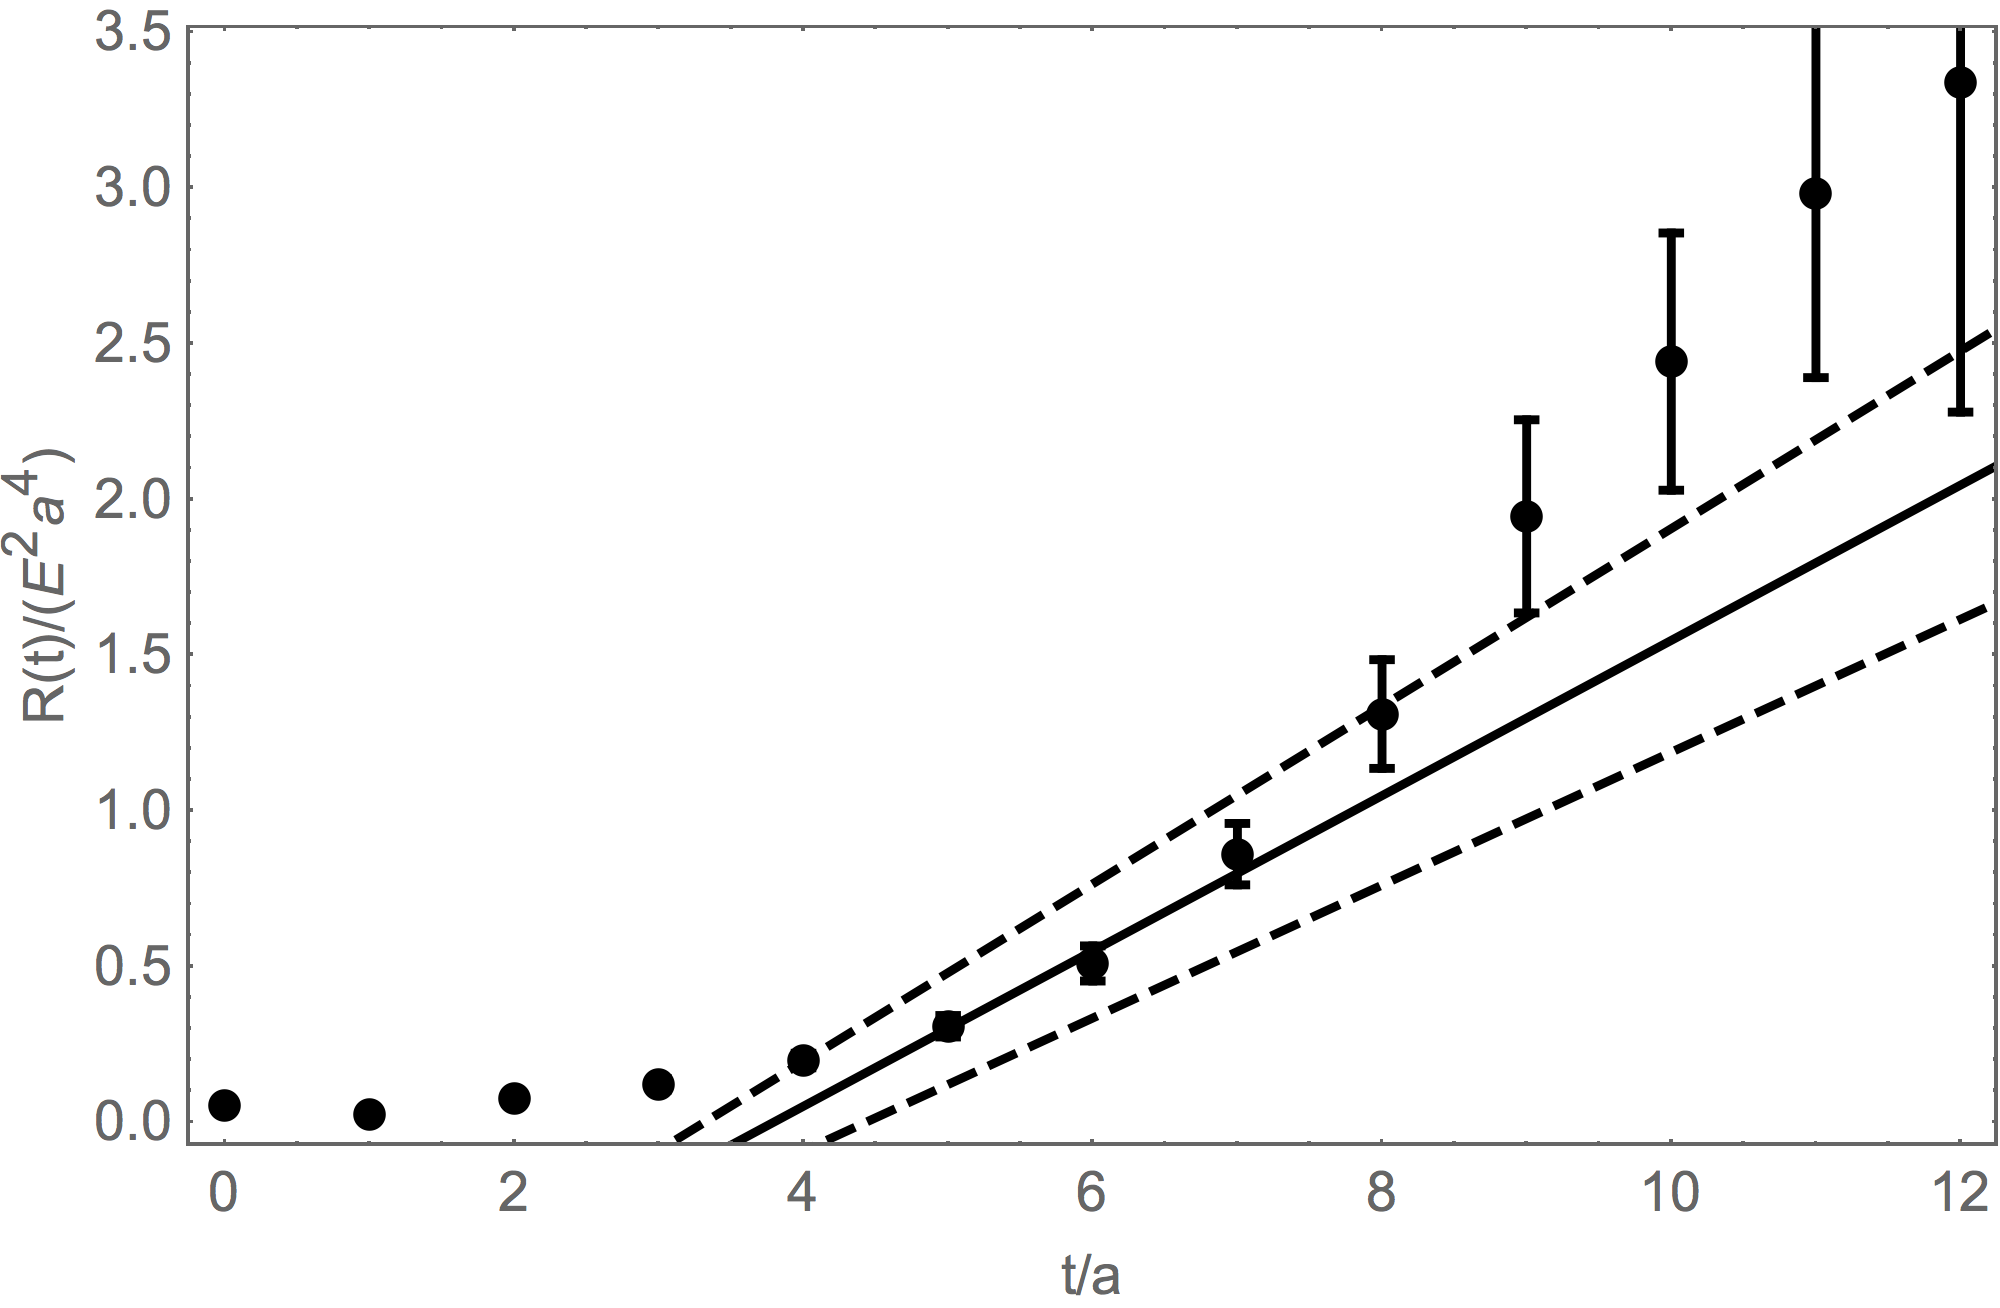
\includegraphics[width=.33\linewidth]{figures/from0LineCS.png}
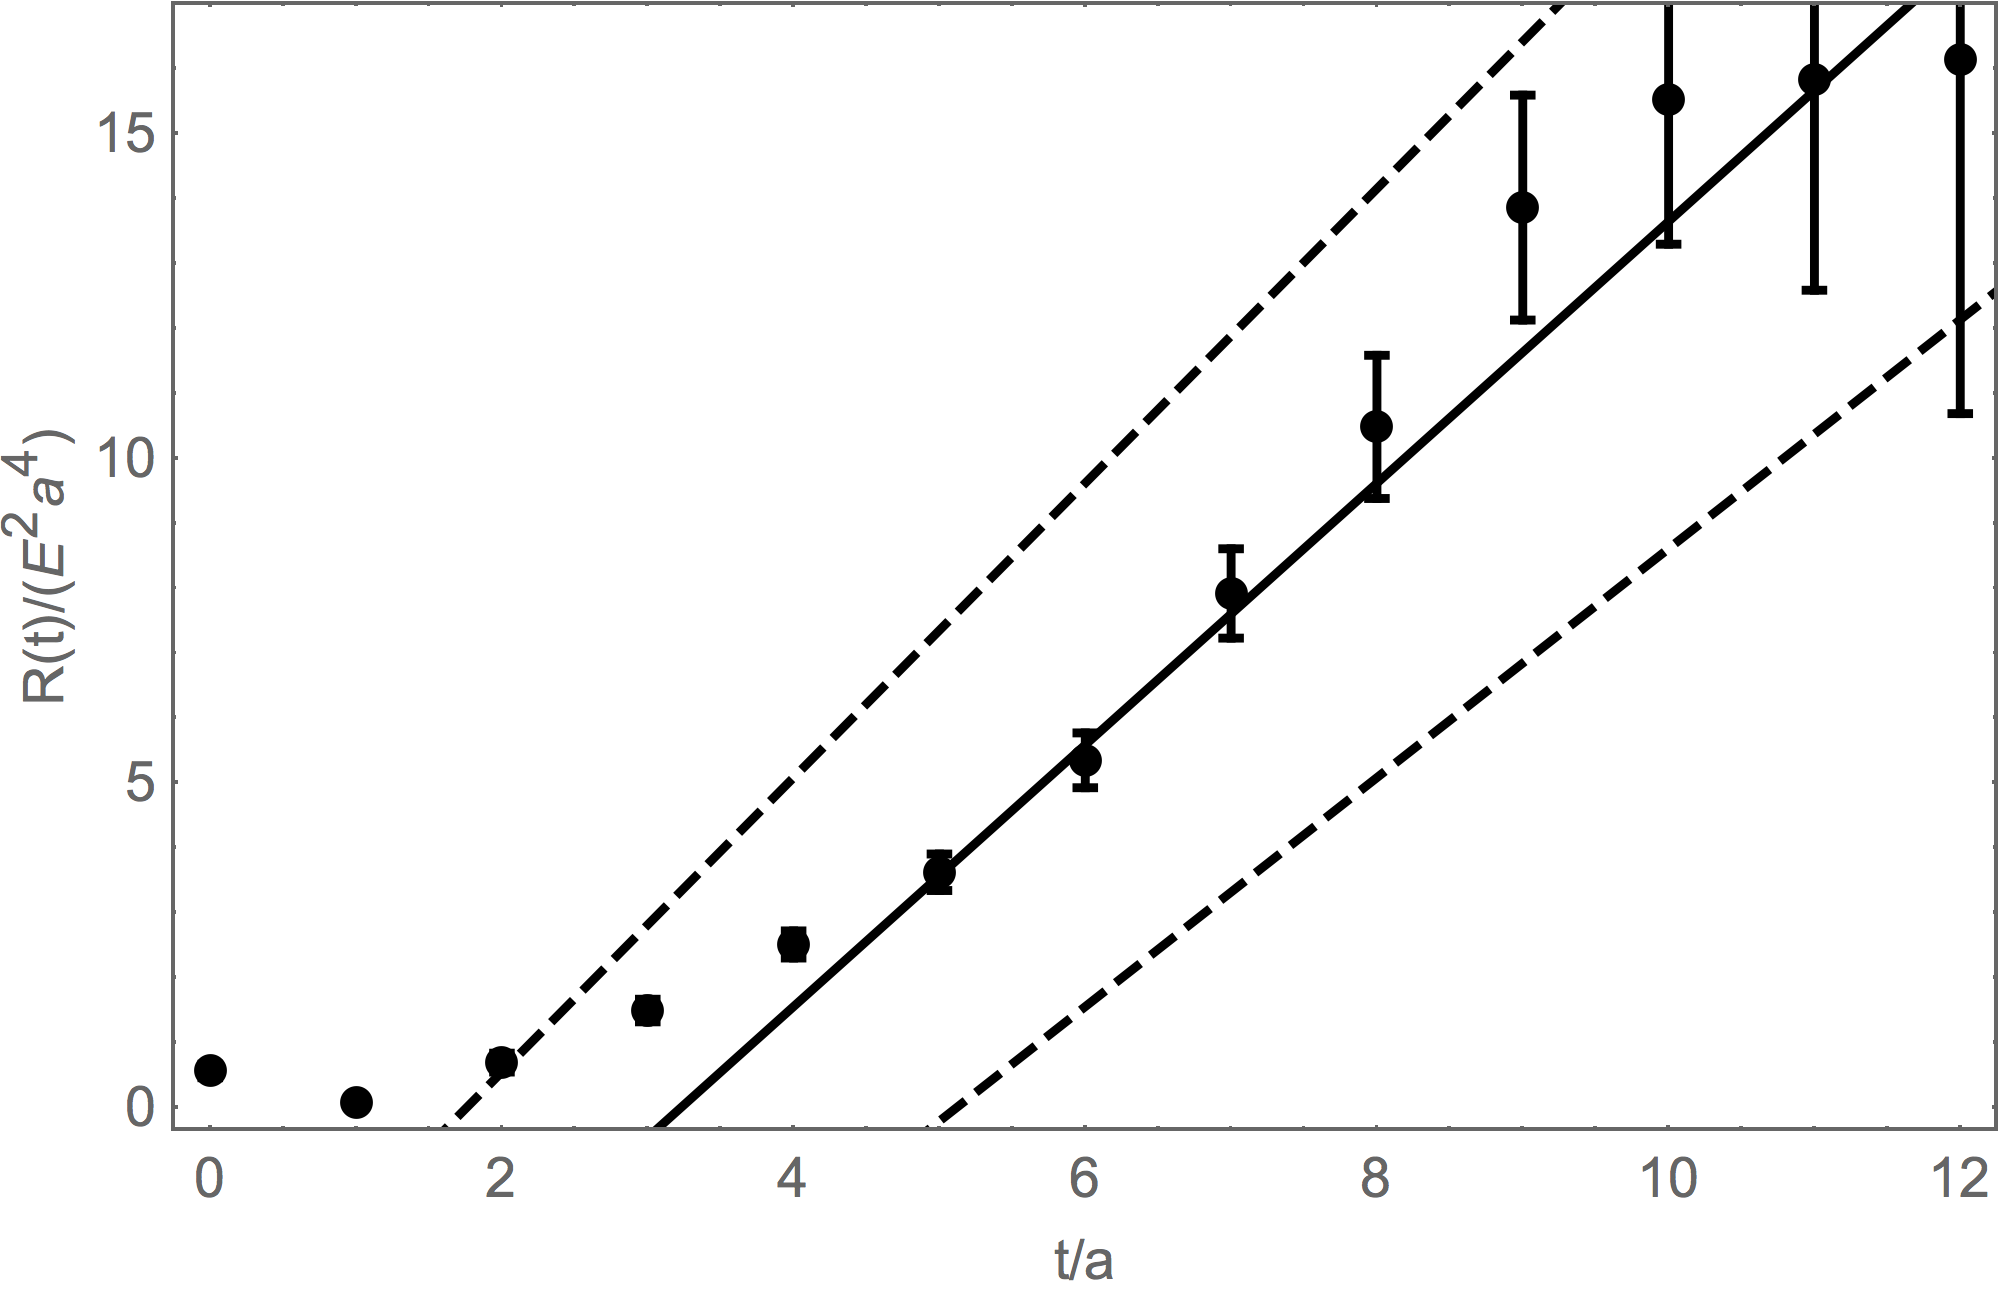
\includegraphics[width=.325\linewidth]{figures/shortLineCS.png}\\
\caption{Correlator ratio $R_2(t)$ and linear fits for the connected diagrams a), b), f), shown in Fig.~\ref{fig:diagrams}, in units of $E^2a^4$. In these plots, the neutron source was placed at the fixed location $t=0$, and the background field, c.f.~\ref{gauge}, was varied with $t_0=6a$, $t_0=0$, $t_0=-10a$ (from left to right). The dashed lines delimit the linear fit uncertainty in the slope.}
\label{fig: alphaconnected}
\end{figure}
%%%%%%%%%%%%%%%%%%%%%%%%%%%%%

%%%%%%%%%Electric Polarizability Results%%%%%
%%%%%%%%%%Multi point Polarizability 10^-4 fm^3%%%%%%
\begin{table}[H]
\begin{center}
    \begin{tabular}{|l|l|l|l|}
    \hline
     Fit range [$t/a$] 					& 5 to 7 		&  4 to 8 		&  3 to 9 \\ \hline
     $\alpha_E$ [$10^{-4}$ $\text{fm}^3$]  	&  0.48(29)      	&  0.57(22)     	& 0.74(16)       \\
								& 0.57(30)		&  0.59(22)	& 0.71(17)		\\ \hline 
     $\alpha_E-\alpha_{FW}$ [$10^{-4}$ $\text{fm}^3$]  	& 0.71(29)   	& 0.79(22)   	&  0.96(16) \\ 
     											& 0.80(30)		& 0.81(22)		& 0.93(17) \\ \hline
    \end{tabular}
\end{center}
\caption{Static electric polarizability  $\alpha_E$ and reduced by the Foldy-Wouthuysen contribution $\alpha_E-\alpha_{FW}$ from the extremal slopes (connected diagrams, $\chi^2$ fits) of the three fitting ranges in units of $10^{-4}$ $\text{fm}^3$. \todo{results from reduced statistics are given in the lower lines}}
\label{tab:ConnectedPolarizabilities}
\end{table}






\subsubsection{Electric polarizability $\alpha_E$, $m_{\pi}$=357 MeV measurements for
connected diagrams in the 1-window analysis}
\label{3571w}
The 1-window analysis considers the $t_0=6a$ data. A cubic function is
fitted, with and without a quadratic term, to assess the inflection point's shift.
In contrast to the 3-window analysis discussed in~\ref{357}, the range 5 to 7 provides
only three points to be fitted, which may not be enough if they are to represent the
cubic generic form of the correlator ratios, shown in figure~\ref{fig:1walpha}. The data ranges from 
4 to 8 and 3 to 9 were considered for the fit, with the latter the preferred range in 
the 1-window analysis.

%%%%%%%%Figure multi point connected cubic fits%%%%%%%%%%%
\begin{figure}[H]
\centering
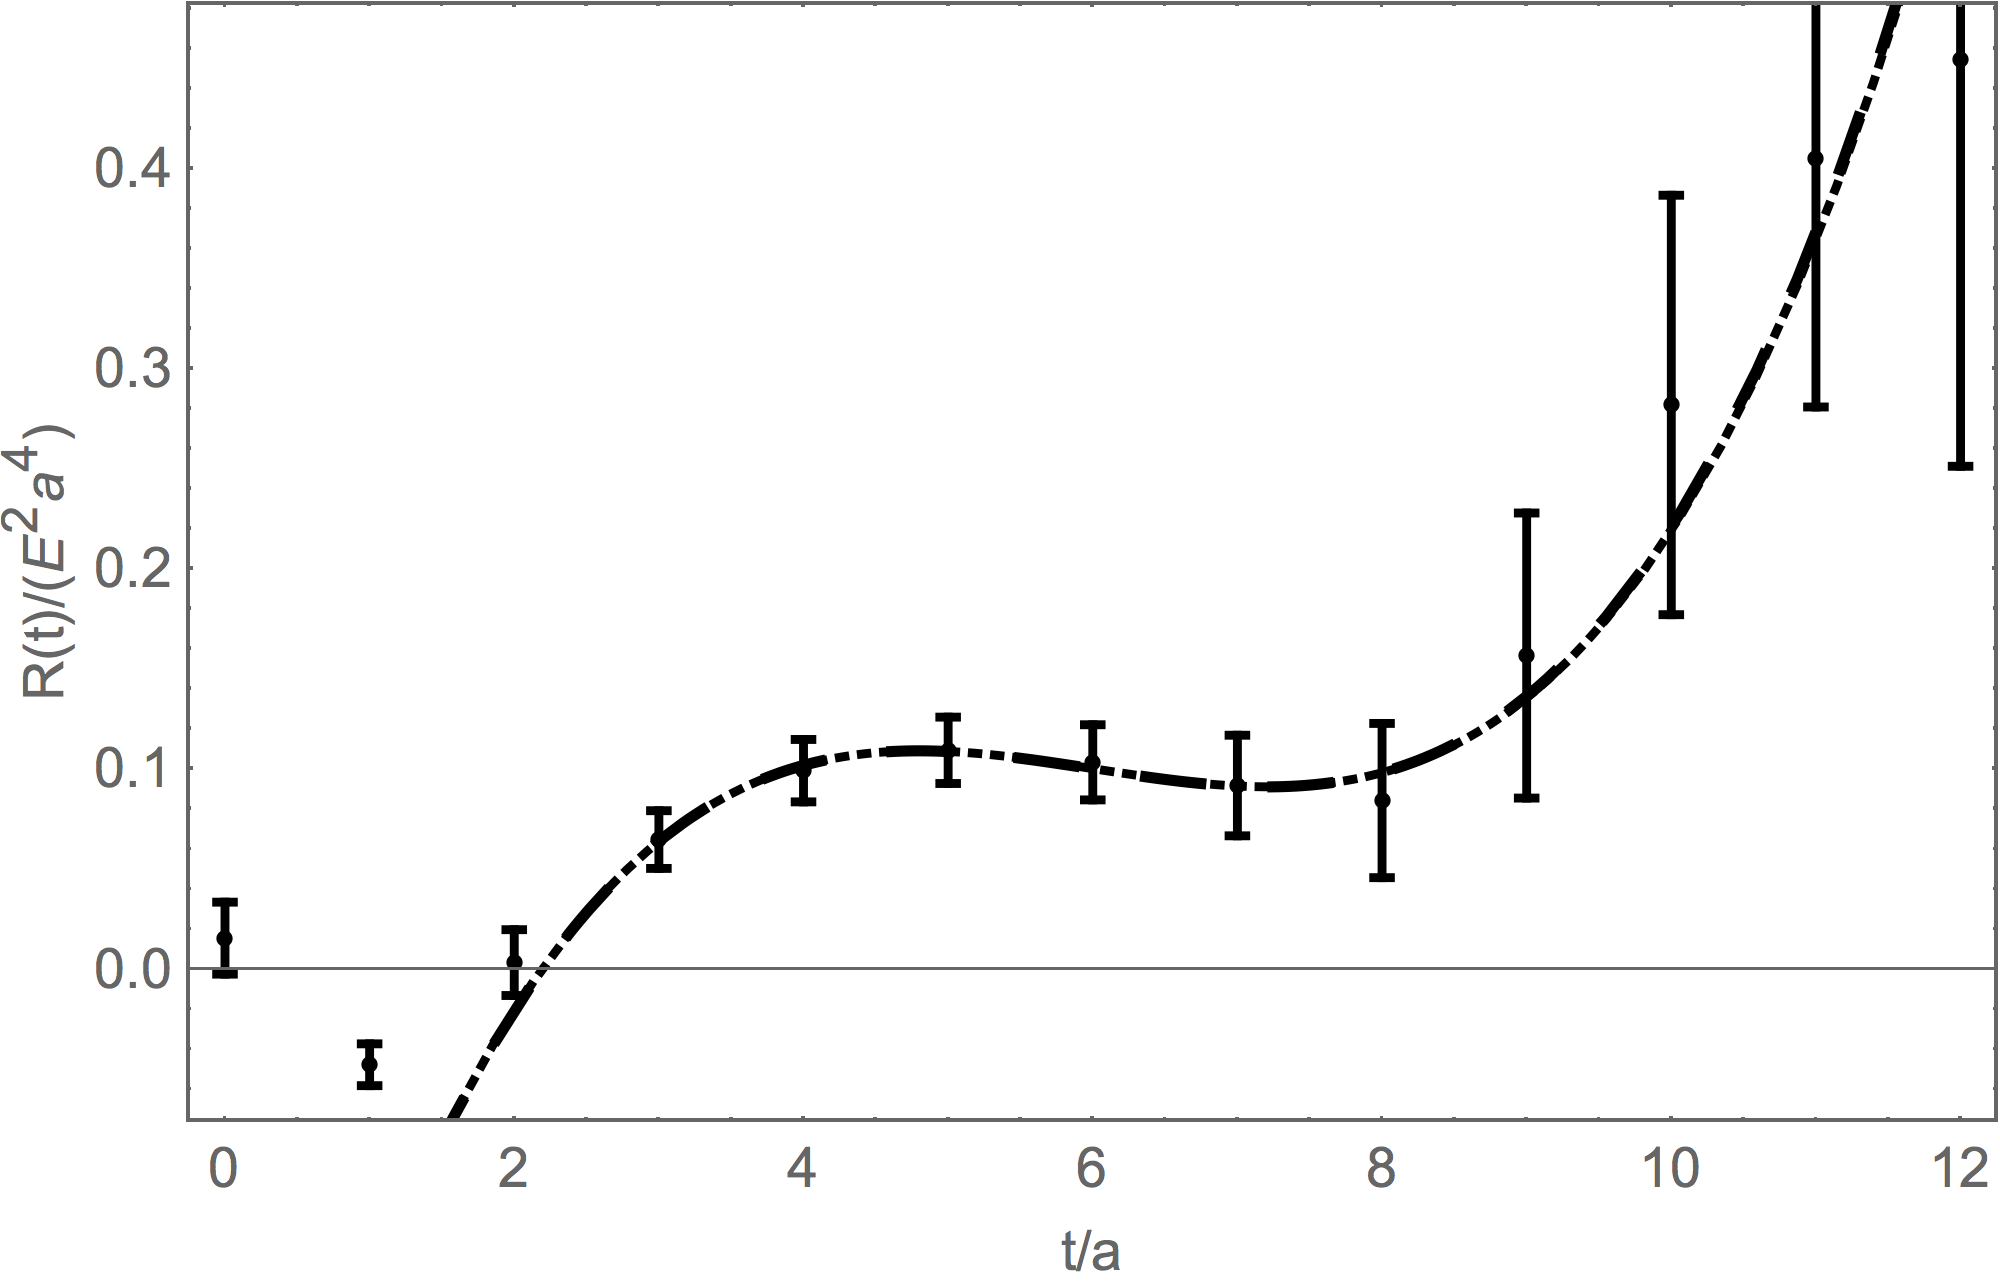
\includegraphics[width=.65\linewidth]{figures/shshQuadCS.png}\\
\caption{Correlator ratio $R_2(t)$ for the connected diagrams a), b), f), shown in Figure ~\ref{fig:diagrams}, in units of $E^2a^4$. A cubic form was fitted with (dotted line) and without (dashed line) a quadratic term.}
\label{fig:1walpha}
\end{figure}
%%%%%%%%%%%%%%%%%%%

Table~\ref{tab:1walphaconnected} shows the inflection points and extremal slopes. The inflection
point positions are compatible with $t/a=6$. The importance of the positions
of these points becomes apparent in light of the possible retardation effects,
which will be discussed below~\ref{retardation}.

%%%%%%%%Table 1-window connected Multi point%%%%%%%%%
\begin{table}[H]
\begin{center}
    \begin{tabular}{|l|l|l|}
    \hline
     Fit range   & 4 to 8   & 3 to 9  \\ \hline
     Inflection point ($t/a$) 		& 6.6(1.2)       	& 6.01(50)      \\ 
     						& 6.55(89) 	& 6.06(45)	\\ \hline
     Extremal slope with   		& -0.012(12)     & -0.0112(88)          \\ 
     a quadratic term [$a^3$]	& -0.016(11)	& -0.0147(87)	\\ \hline
     Extremal slope w/o   		& -0.012(10)     & -0.01123(95)   \\ 
     a quadratic term [$a^3$]	& -0.016(10)	& -0.0150(93)	\\ \hline
    \end{tabular}
\end{center}
\caption{Inflection points and extremal slopes for the $\chi^2$ cubic fits in the 1-window analysis for connected diagrams a), b), f), shown in Figure ~\ref{fig:diagrams}. \todo{results from reduced statistics are given in the lower lines}}
\label{tab:1walphaconnected}
\end{table}
%%%%%%%%%%%%%%%%%%%%%%%%%%%%%%%%%%%
 

The  electric polarizability from the 1-window
analysis is presented in Table~\ref{tab:1wElectricPolarizabilityConn}. 
These measurements are consistent with those presented in 
Table~\ref{tab:ConnectedPolarizabilities} for the 3-window analysis of the data.
Comparing these two result tables allows one to
identify smaller statistical errors in the 3-window analysis than in 
the 1-window counterpart. However, it is not guaranteed that the
correlator ratio $R_2(t)$ behaves in a purely cubic way, 
especially if scrutinized far away from the inflection point. \textcolor{red}
{In this regard, there is an unquantified systematic uncertainty in the 3-window analysis.}

%%%%%%%%%Static polarizability 1-window%%%%%%%%%%%%%%%
\begin{table}[H]
\begin{center}
    \begin{tabular}{ | l | c | c | }
    \hline
     Fit range ($t/a$) & $\alpha$ [$10^{-4}$ $\text{fm}^3$]    & $\alpha-\alpha_{FW}$ [$10^{-4}$ $\text{fm}^3$]       \\ 
     \hline
        (with quadratic) 4 to 8&   0.46(46)       &    0.69(46)          \\ \hline
     3 to 9 &  0.43(34)        &     0.65(36)          \\ \hline\hline
 (without quadratic) 4 to 8 &   0.46(39)       &    0.68(39)          \\ \hline
     3 to 9 &   0.43(36)        &     0.65(36)          \\ \hline
    \end{tabular}
\end{center}
\caption{Static electric polarizability  $\alpha$ and reduced by the Foldy-Wouthuysen contribution $\alpha-\alpha_{FW}$ from the extremal slopes (1-window analysis, connected diagrams, $\chi^2$ fits) of the two fitting ranges in units of $10^{-4}$ $\text{fm}^3$. \todo{'point' results?}}
\label{tab:1wElectricPolarizabilityConn}
\end{table}
%%%%%%%%%%%%%%%%%%

\subsubsection{Electric polarizability $\alpha_E$ including all diagrams in the 3-window analysis}
\label{3573wAll}
The 3-window analysis was also performed for all diagrams, connected and disconnected,
shown in~\ref{fig:diagrams}. The correlator ratios $R_2(t)$ are shown in figure~\ref{fig:Correlators3wAll}. 
The plots roughly correspond to the cubic behavior depicted in~\ref{fig:CubicAll}.
 The inflection points and extremal slopes were obtained for 
 the fitting ranges 5 to 7, 4 to 8, 3 to 9, as shown in~\ref{tab:ExtremaMultiPointAll}.
%%%%%%%%%All diagrams R(t)%%%%%%
\begin{figure}[H]
\centering
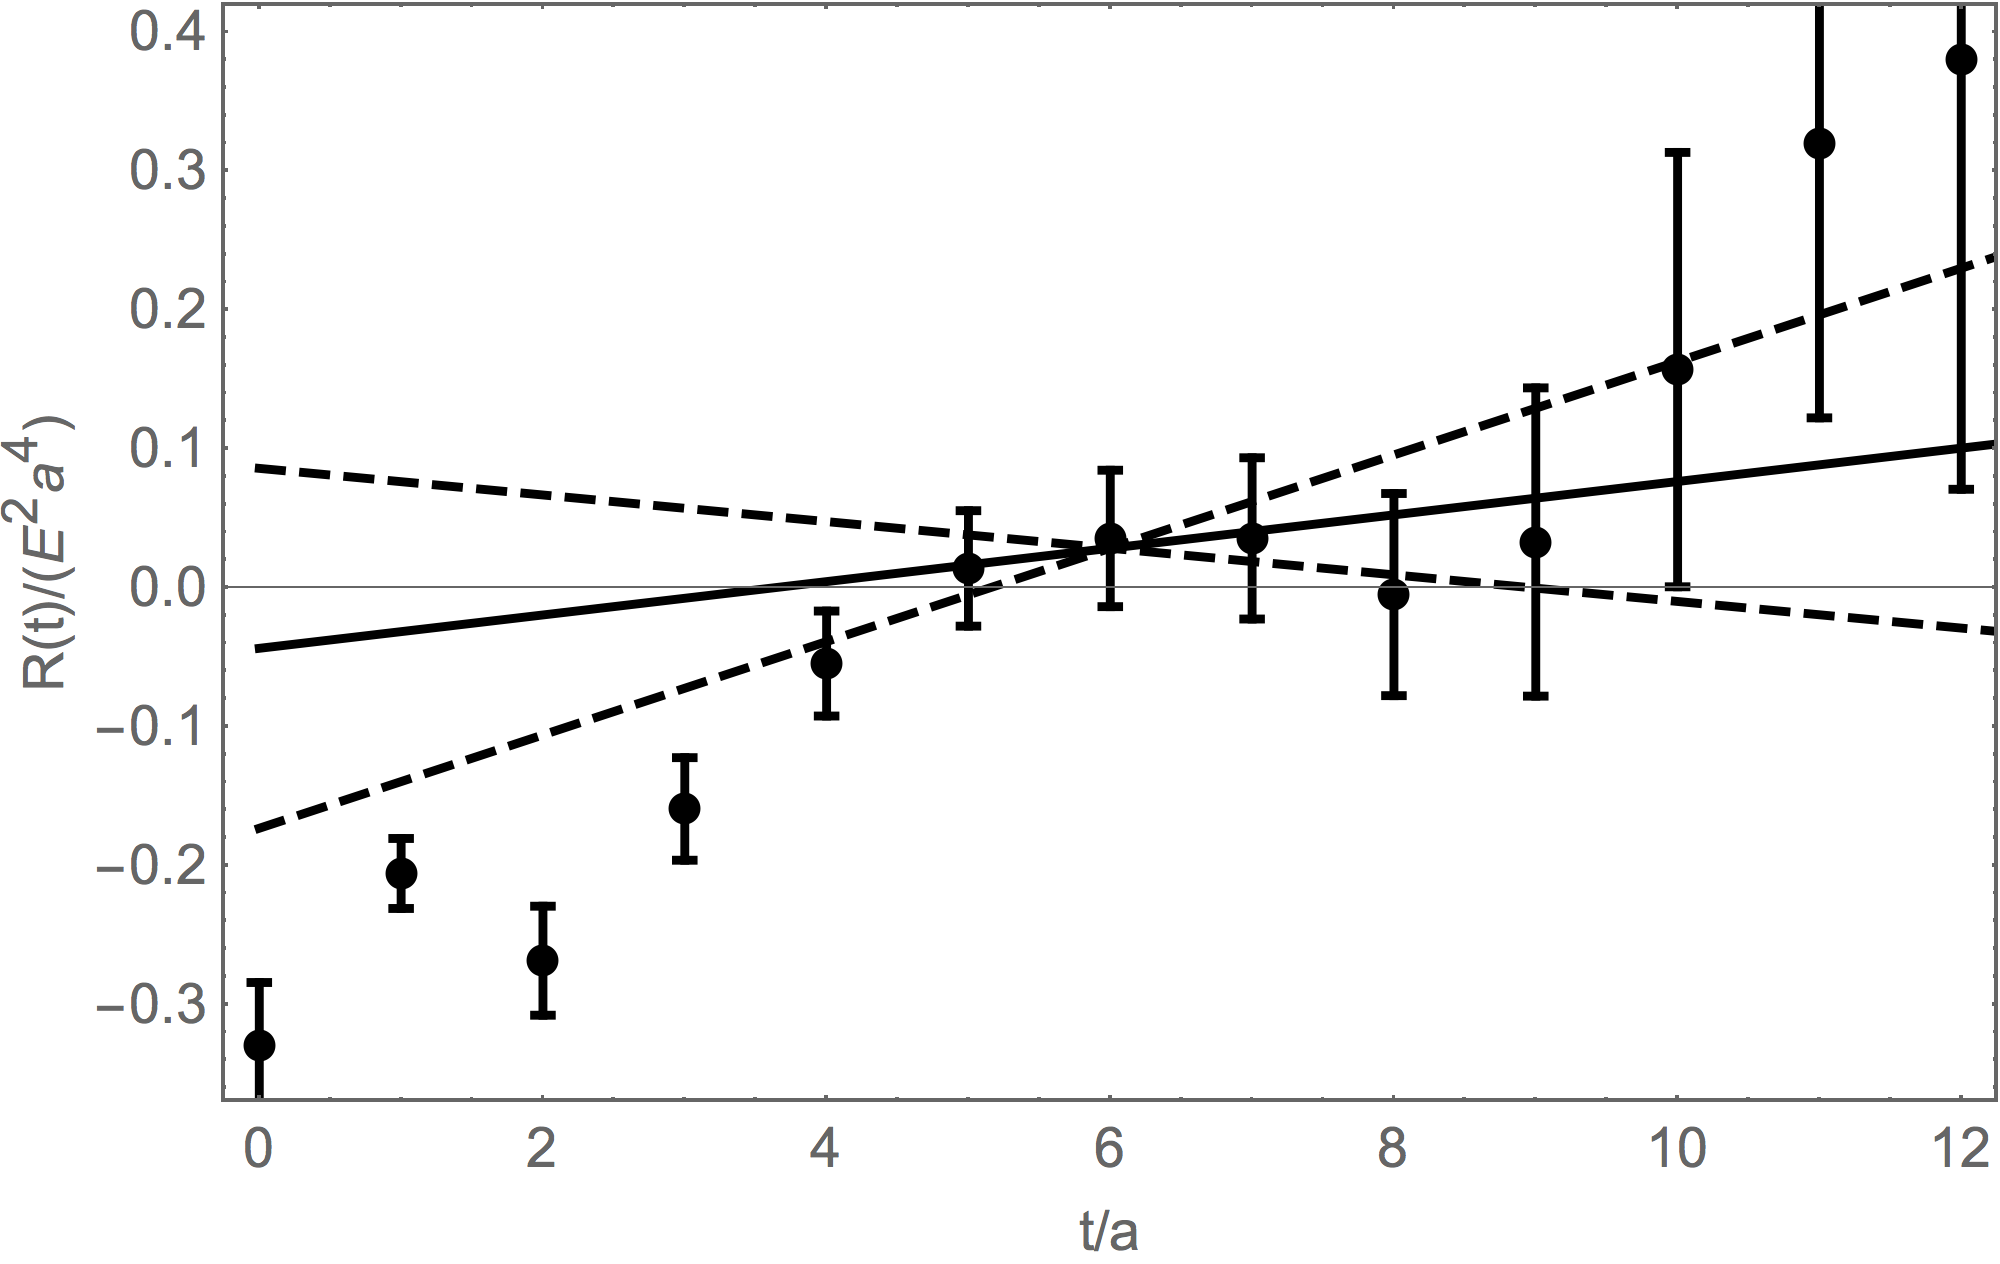
\includegraphics[width=.333\linewidth]{figures/FullshshLineCS.png}
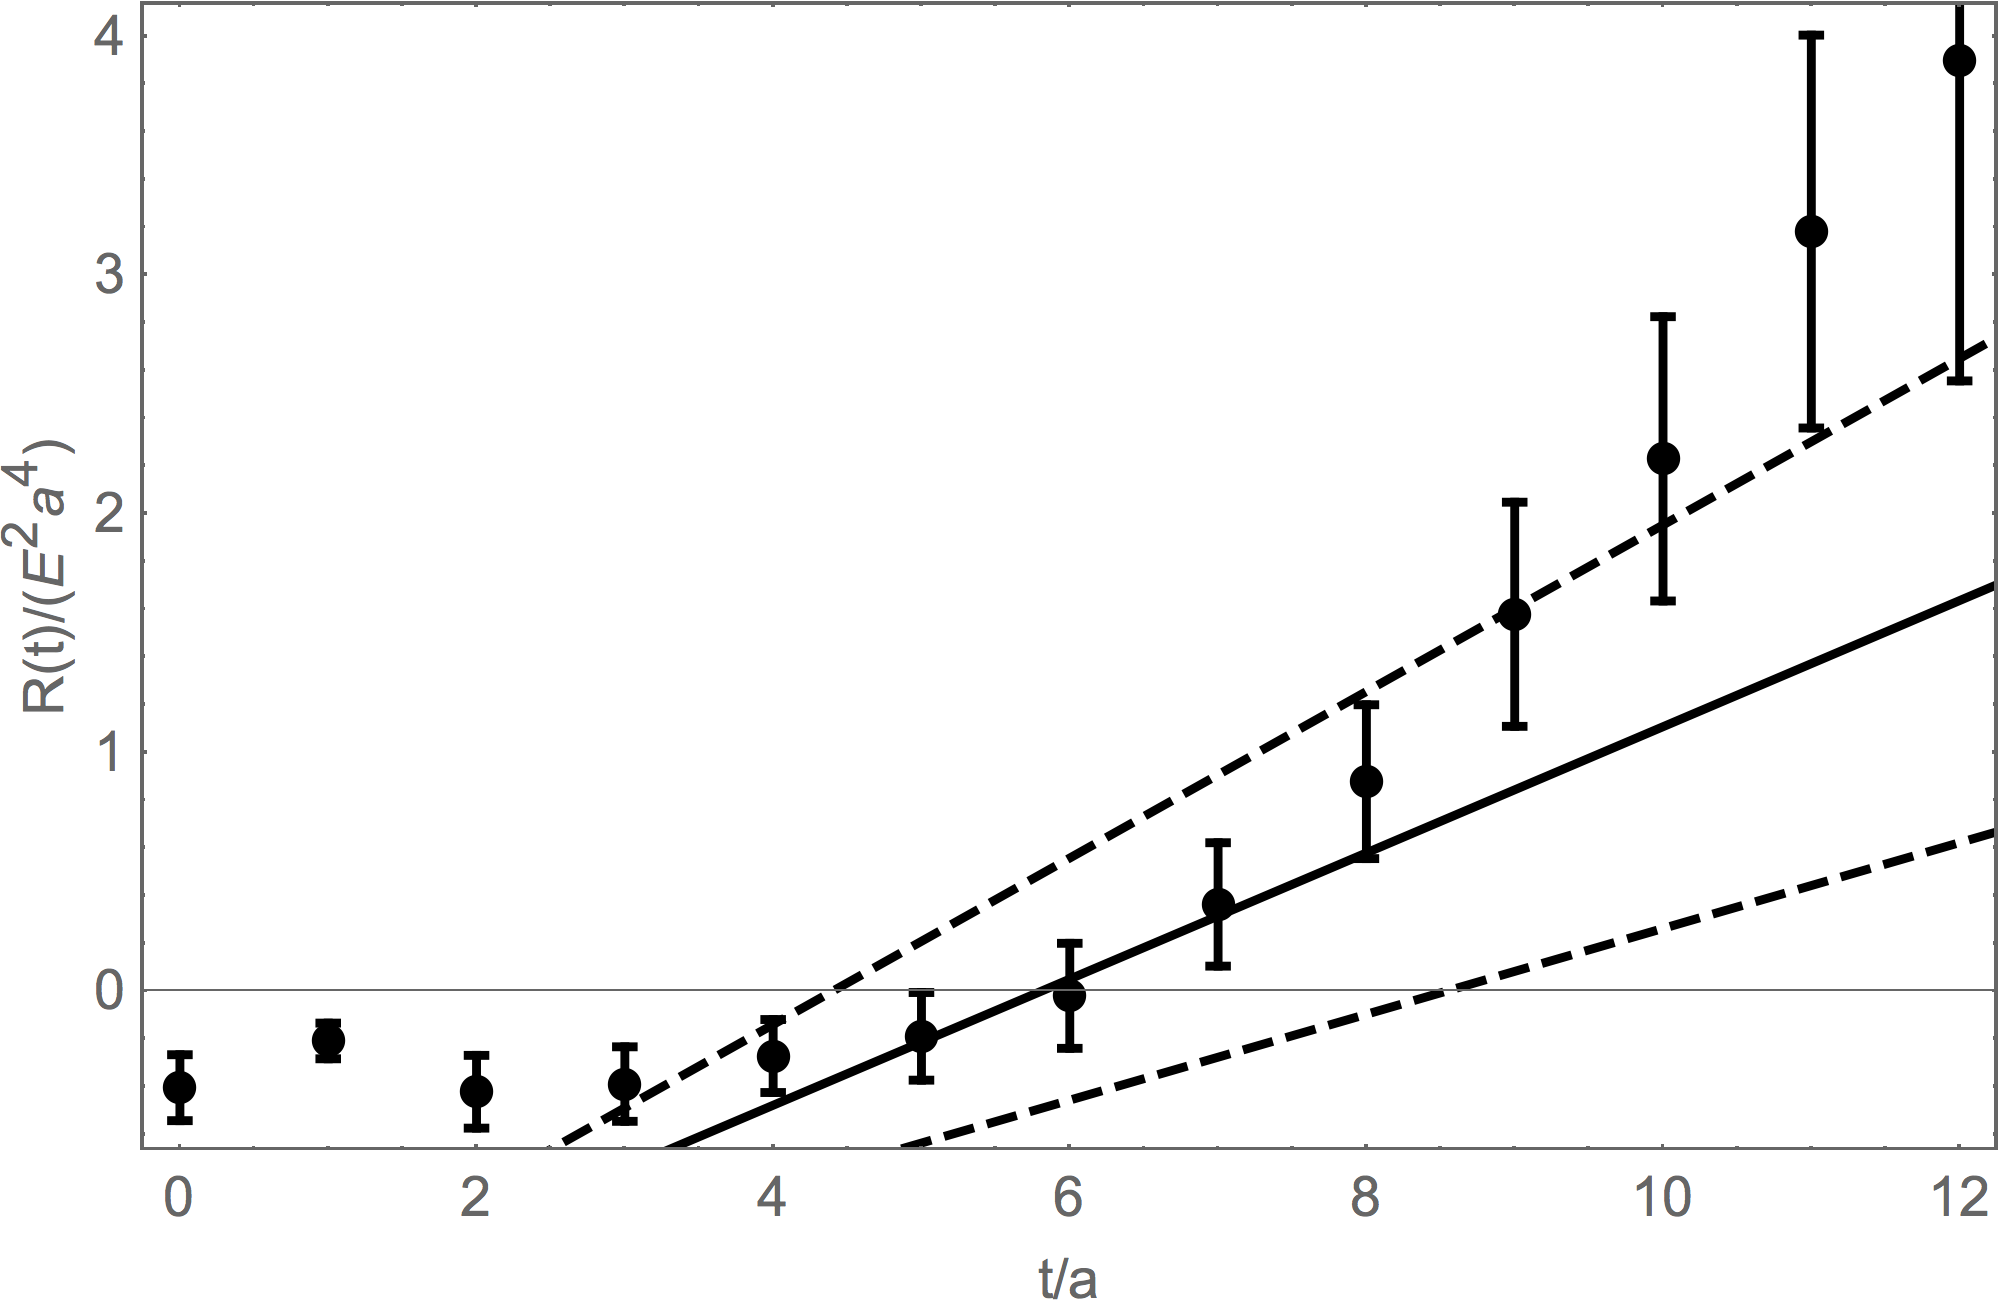
\includegraphics[width=.32\linewidth]{figures/Fullfrom0LineCS.png}
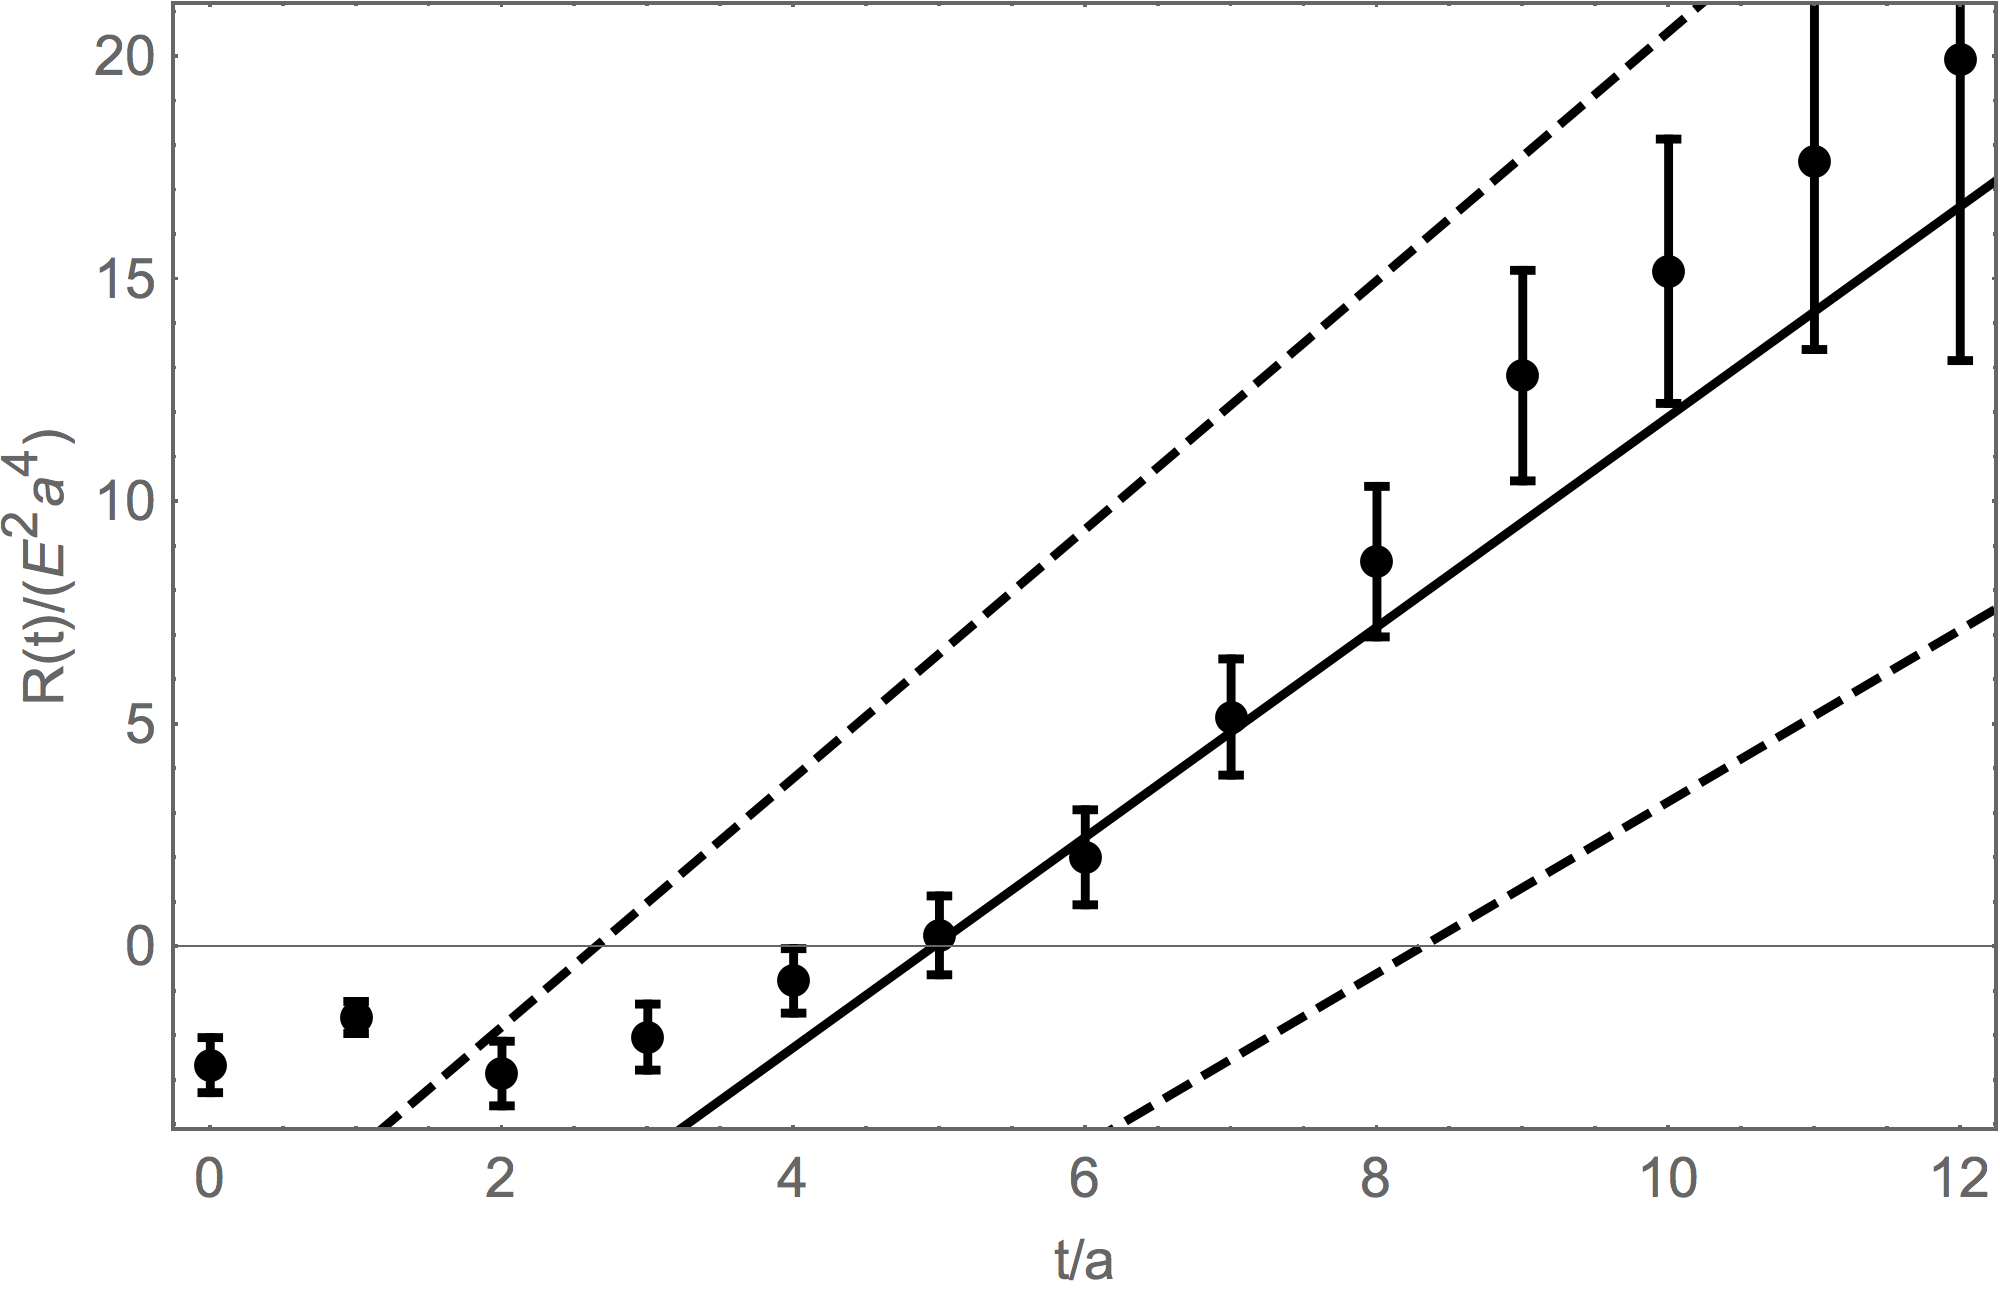
\includegraphics[width=.325\linewidth]{figures/FullshortLineCS.png}\\
\caption{Correlator ratio $R_2(t)$ for all diagrams shown in Figure ~\ref{fig:diagrams}, in units of $E^2a^4$. In these plots, the neutron source was placed at the fixed location $t=0$, and the background field, c.f.~\ref{gauge}, was varied with $t_0=6a$, $t_0=0$, $t_0=-10a$ (from left to right).The dashed lines delimit the linear fit uncertainty in the slope.}
\label{fig:Correlators3wAll}
\end{figure}
%%%%%%%%%%%%%%%%%%%%%%%%%%%%%
%%%%%%%%Generic Cubic Behavior%%%%%%%%%
\begin{figure}[H]
\centering
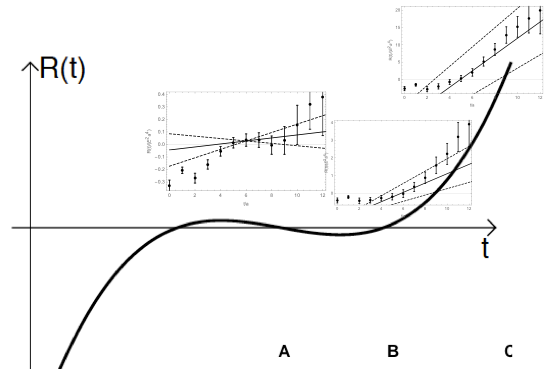
\includegraphics[width=.65\linewidth]{figures/full3window.png}
\\
\caption{3-window generic cubic behavior for all diagrams. The plots in figure~\ref{fig:Correlators3wAll} 
are the three time windows shown here in their approximate positions.}
\label{fig:CubicAll}
\end{figure}
%%%%%%%%%%%%%%%%%%%%%%%%%%%%%

%%%%%Full EXTREMUM TABLE%%%%%%
\begin{table}[H]
\begin{center}
    \begin{tabular}{ | l | l| l | l |}
    \hline
     Fit range [$t/a$] 			& 5 to 7   		& 4 to 8   		& 3 to 9  \\ \hline
     Inflection point [$t/a$]		&  6.99(39)   	&  6.97(38)    	& 7.12(34)    \\ 
     						& 6.90(87)		& 7.12(91)		& 7.7(1.0)	\\ \hline
     Extremal slope [$a^3$]		&   -0.002(24)   & 0.001(19)   	& 0.005(16)  \\
     						& -0.006(61)	& -0.023(50)	& -0.037(46) \\ \hline
    \end{tabular}
\end{center}
\caption{Inflection points and extremal slopes for the $\chi^2$ linear fits in the 3-window analysis with parabola minimum lift correction, for all connected and disconnected diagrams. \todo{results from reduced statistics are given in the lower lines}}
\label{tab:ExtremaMultiPointAll}
\end{table}
%%%%%%%%%%%%%%%%%%%%
%%%%%%%%%%%%%%%%%%%%%%%%%
The electric polarizability for all diagrams was calculated from 
the results in table~\ref{tab:ExtremaMultiPointAll}
for the selected fitting ranges, with and without the Foldy-Wouthuysen contribution.
Table~\ref{tab:FullPolarizabilities} shows the electric polarizability 
measurements for the ``multi point" dataset.

%%%%%%%%%%All diagramsPolarizability 10^-4 fm^3%%%%%%
\begin{table}[H]
\begin{center}
    \begin{tabular}{|l|l|l|l|}
    \hline
     Fitting range ($t/a$) 						&  5 to 7 	&  4 to 8 	& 3 to 9	\\ \hline
     $\alpha_E$ [$10^{-4}$ $\text{fm}^3$]   			& 0.07(92)	&-0.04(72)& 0.19(72) \\
     										&	&	&  \\ \hline
     $\alpha_E-\alpha_{FW}$ [$10^{-4}$ $\text{fm}^3$] 	& 0.29(92)	&-0.19(63)& 0.04(63) \\ 
 										&	&	&	\\ \hline
    \end{tabular}
\end{center}
\caption{Static electric polarizability  $\alpha_E$ and static electric polarizability minus Foldy-Wouthuysen contribution $\alpha_E-\alpha_{FW}$ from the extremal values (all diagrams, $\chi^2$ fits, ``multi point" dataset) of the three fitting ranges in units of $10^{-4}$ $\text{fm}^3$. \todo{'point' results?}}
\label{tab:FullPolarizabilities}
\end{table}
%%%%%%%%%%%%%%%%%%%%%%%%%%%%%


\subsubsection{Electric polarizability $\alpha_E$ including all diagrams in the 1-window analysis}
\label{3571wAll}

%%%%%%%%%%%%%%%%%%%%%%%%%%%%%%%%%%%
\begin{figure}[H]
\centering
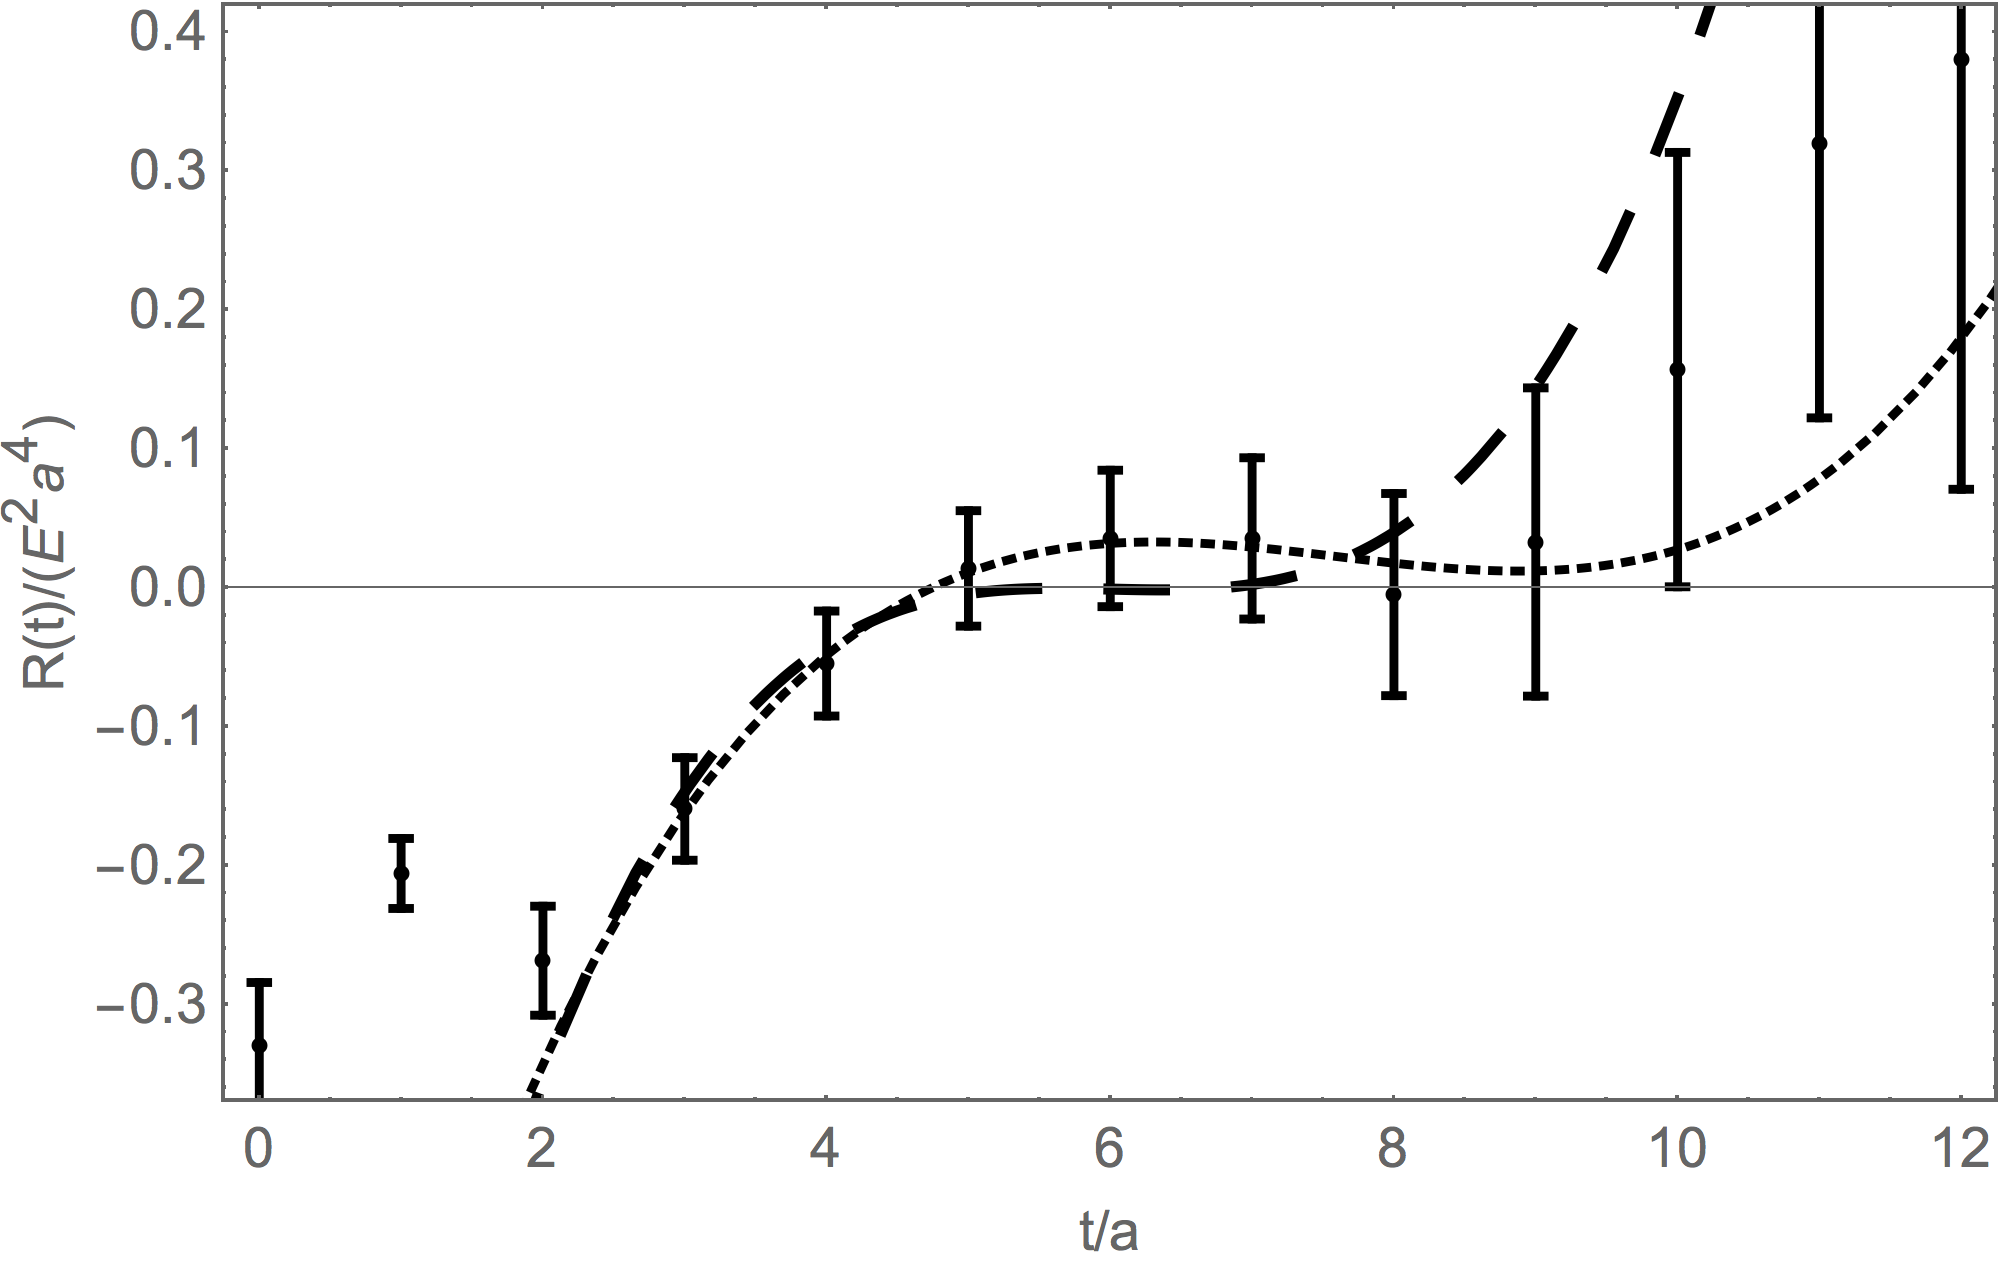
\includegraphics[width=.65\linewidth]{figures/shshQuadCSFull.png}\\
\caption{Correlator ratio $R_2(t)$ for all diagrams (connected and disconnected) shown in Figure ~\ref{fig:diagrams}, in units of $E^2a^4$. A cubic form was fitted with (dotted line) and without (dashed line) a quadratic term.}
\label{fig:1walphafull}
\end{figure}

%%%%%%%%Table 1-window full Multi point%%%%%%%%%
\begin{table}[H]
\begin{center}
    \begin{tabular}{ | l | l | l | }
    \hline
     Fit range [$t/a$]   			& 4 to 8   & 3 to 9  \\ \hline
     Inflection point [$t/a$]		& 12(55)   & 7.6(2.0)    \\ 
     						& 6.4(2.0)	& 7(82) \\\hline
     Extremal slope with   		&  -0.10(97)  &  -0.012(38) \\
     a quadratic term [$a^3$]	& 0.012(60) & 0.01(23) \\ \hline
     Extremal slope w/o		&  -0.000(25)   &  -0.002(22) \\
     a quadratic term [$a^3$]	& 0.011(60) & 0.005(53) \\ \hline
    \end{tabular}
\end{center}
\caption{Inflection points and extremal slopes for the $\chi^2$ cubic fits in the 1-window analysis for all connected and disconnected diagrams. \todo{results from reduced statistics are given in the lower lines}}
\label{tab:1walphafull}
\end{table}
%%%%%%%%%%%%%%%%%%%%%%%%%%%%%%%%%%%

%%%1-w polarizabilities goes here%%%
%%%%%%%%%Static polarizability 1-window Multipoint%%%%%%%%%%%%%%%
\begin{table}[H]
\begin{center}
    \begin{tabular}{|l||c|c||c|c||}
    \hline	& \multicolumn{2}{c}{with quadratic term} & \multicolumn{2}{c}{w/o quadratic term} \\ \hline
     Fit range [$t/a$)]						& 4 to 8 	& 3 to 9 	& 4 to 8 	& 3 to 9 \\ \hline 
     $\alpha_E$ [$10^{-4}$ $\text{fm}^3$]    		& 4(37)	& 0.5(1.4) 	& 0.01(94)	& 0.09(83) \\ \hline     
     $\alpha_E-\alpha_{FW}$ [$10^{-4}$ $\text{fm}^3$]& 4(37)	&  0.7(1.4)	& 0.23(94)	& 0.31(83) \\ \hline
    \end{tabular}
\end{center}
\caption{Static electric polarizability  $\alpha$ and reduced by the Foldy-Wouthuysen contribution $\alpha-\alpha_{FW}$ from the extremal values (1-window analysis, connected and disconnected diagrams, $\chi^2$ fits) of the two fit ranges in units of $10^{-4}$ $\text{fm}^3$. \todo{point results?}}
\label{tab:1wElectricPolarizabilityAllMultiPoint}
\end{table}
%%%%%%%%%%%%%%%%%%

\section{Retardation effects}
\label{retardation}
In a time-independent Hamiltonian scenario, neutron excited states are present
in the hadron source. These excited states decay and eventually only the ground state
remains. This effect manifests in the three-point function; there is a plateau in the
neutron energy. 
In our analysis, the Hamiltonian is time-dependent; excited states 
come from the hadron source but are also continuously produced by the time 
evolution, i.e., a fast-changing electric field. This time dependence could be
extracted from a time-dependent, expressed in Euclidean time, perturbation theory
analysis. A fit function would contain the effects from excited states from the hadron
source and the excited states generated by the electromagnetic perturbation, i.e.,
the time-varying electric field. Whereas in a time-independent Hamiltonian case there
is no inflection point shift, in our time-dependent case, one of the indicators 
of the excited state presence is a consistent shift in the inflection point. However, we argue 
that there is no significant slope variation between $t=6a$ and the inflection point 
in the three-window analysis. In the one-window analysis the shift in the inflection point is
not resolvable. At the same time, the slope values at $t=6a$ and at the shifted inflection point also
agree within uncertainties. Thus, \textcolor{red}{no excited state analysis is required for the results in our work}.

\subsection{Slope values at $t=6a$ for the connected diagrams in the 
3-window and 1-window analyses}
\label{ritardation_connected}
Significant retardation effects would be suggested by non-negligible deviations
of the slope at the shifted inflection point with respect to the slope at $t/a=6$. 
Our results show compatible slope values at these points. Note that in our three-
window analysis the fit of choice is $t/a=$ 5 to 7, and the slopes agree within 
uncertainties even though the inflection points are shifted to the right, as shown
in Figure~\ref{fig:shifinflecconn}.
%%%% extremal, position and slope, Multi point, connected diagrams%%%
\begin{table}[H]
\begin{center}
    \begin{tabular}{ | l | c | c | c |}
    \hline
     Fit range [$t/a$] & 5 to 7    & 4 to 8 & 3 to 9      \\ 
     \hline
        	Inflection point [$t/a$] &   6.43(24)         &      6.74(19)    &    7.28(13)   \\ \hline
        Extremal slope [$a^3$] &    -0.0127(77)        &     -0.0149(58)    &      -0.0194(42) \\ \hline
 	Slope at $t=6a$ [$a^3$] &    -0.0111(86)        &     -0.0109(68)   &     -0.0083(52)   \\ \hline
    
    \end{tabular}
\end{center}
\caption{Inflection points, extremal slope and slope at $t=6a$ for the $\chi^2$
linear fits for connected diagrams in the 3-window analysis with parabola minimum lift correction.}
\label{tab:Retardation3wMultiPoint}
\end{table}

%%%%%%%%%%%%%%%%%%%%%%%%%%%%%%%%%%%%%%

\begin{figure}[H]
  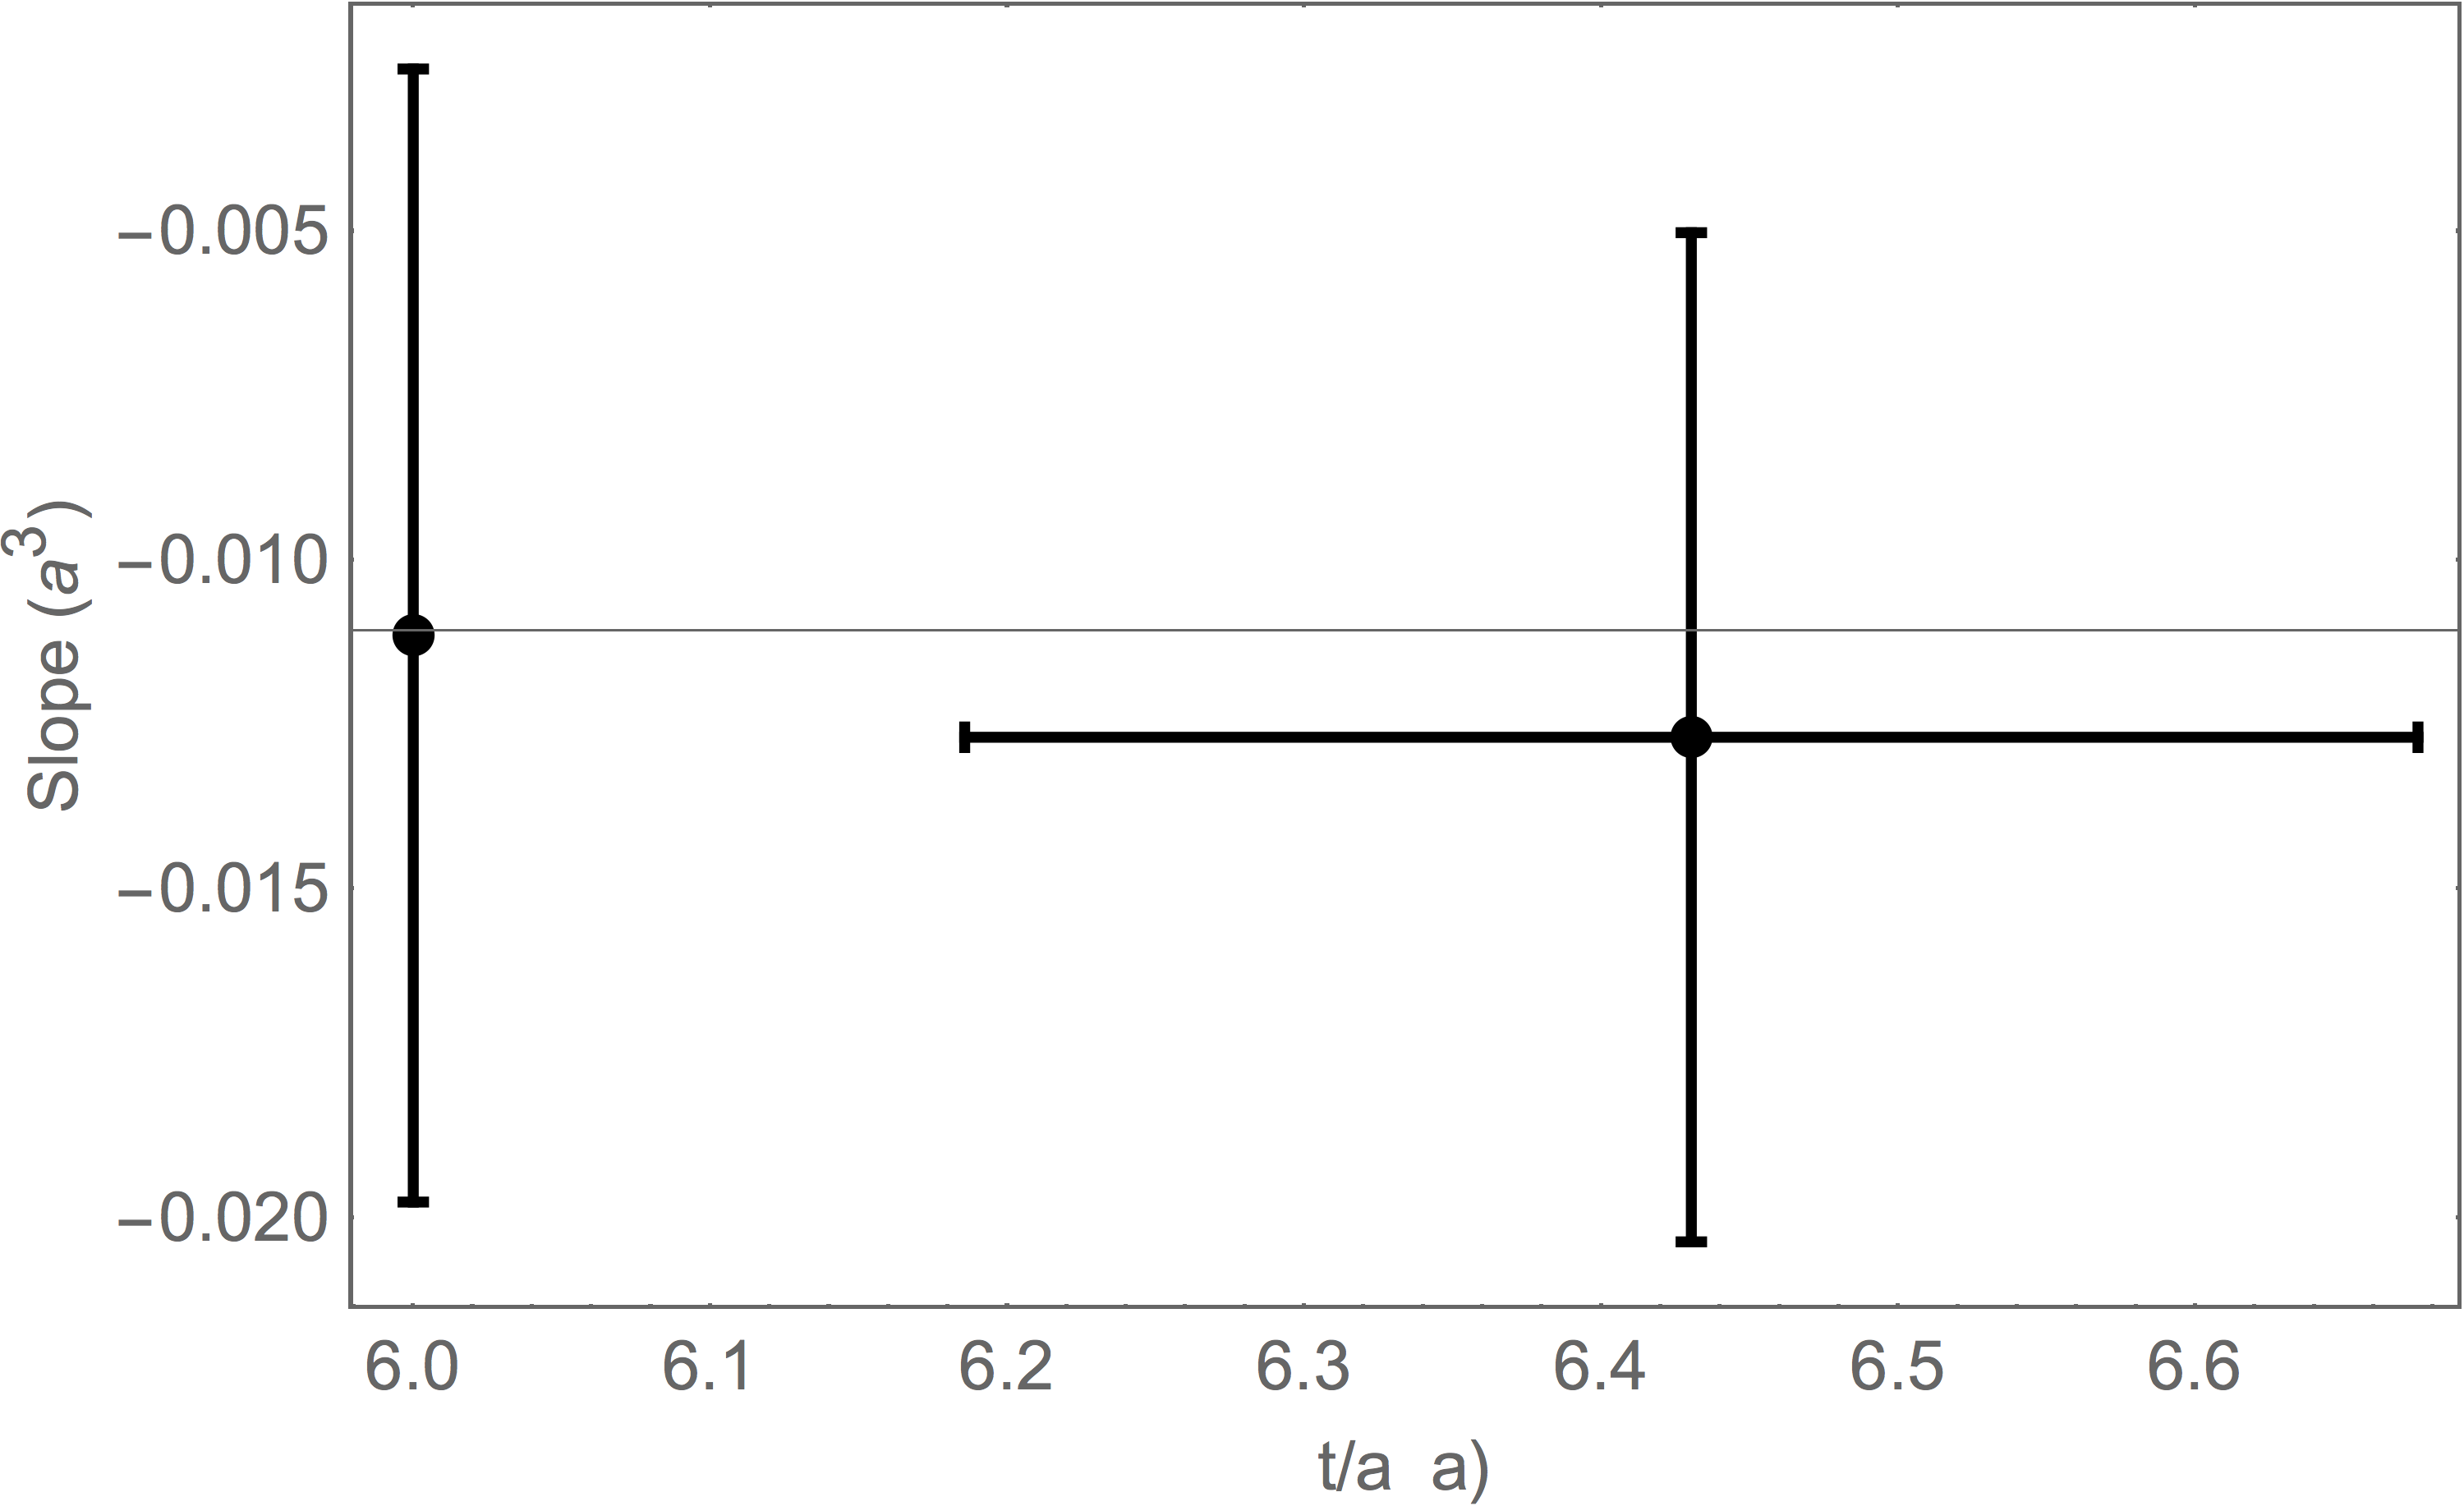
\includegraphics[width=.33\linewidth]{figures/3wC5-7Chi.png}
  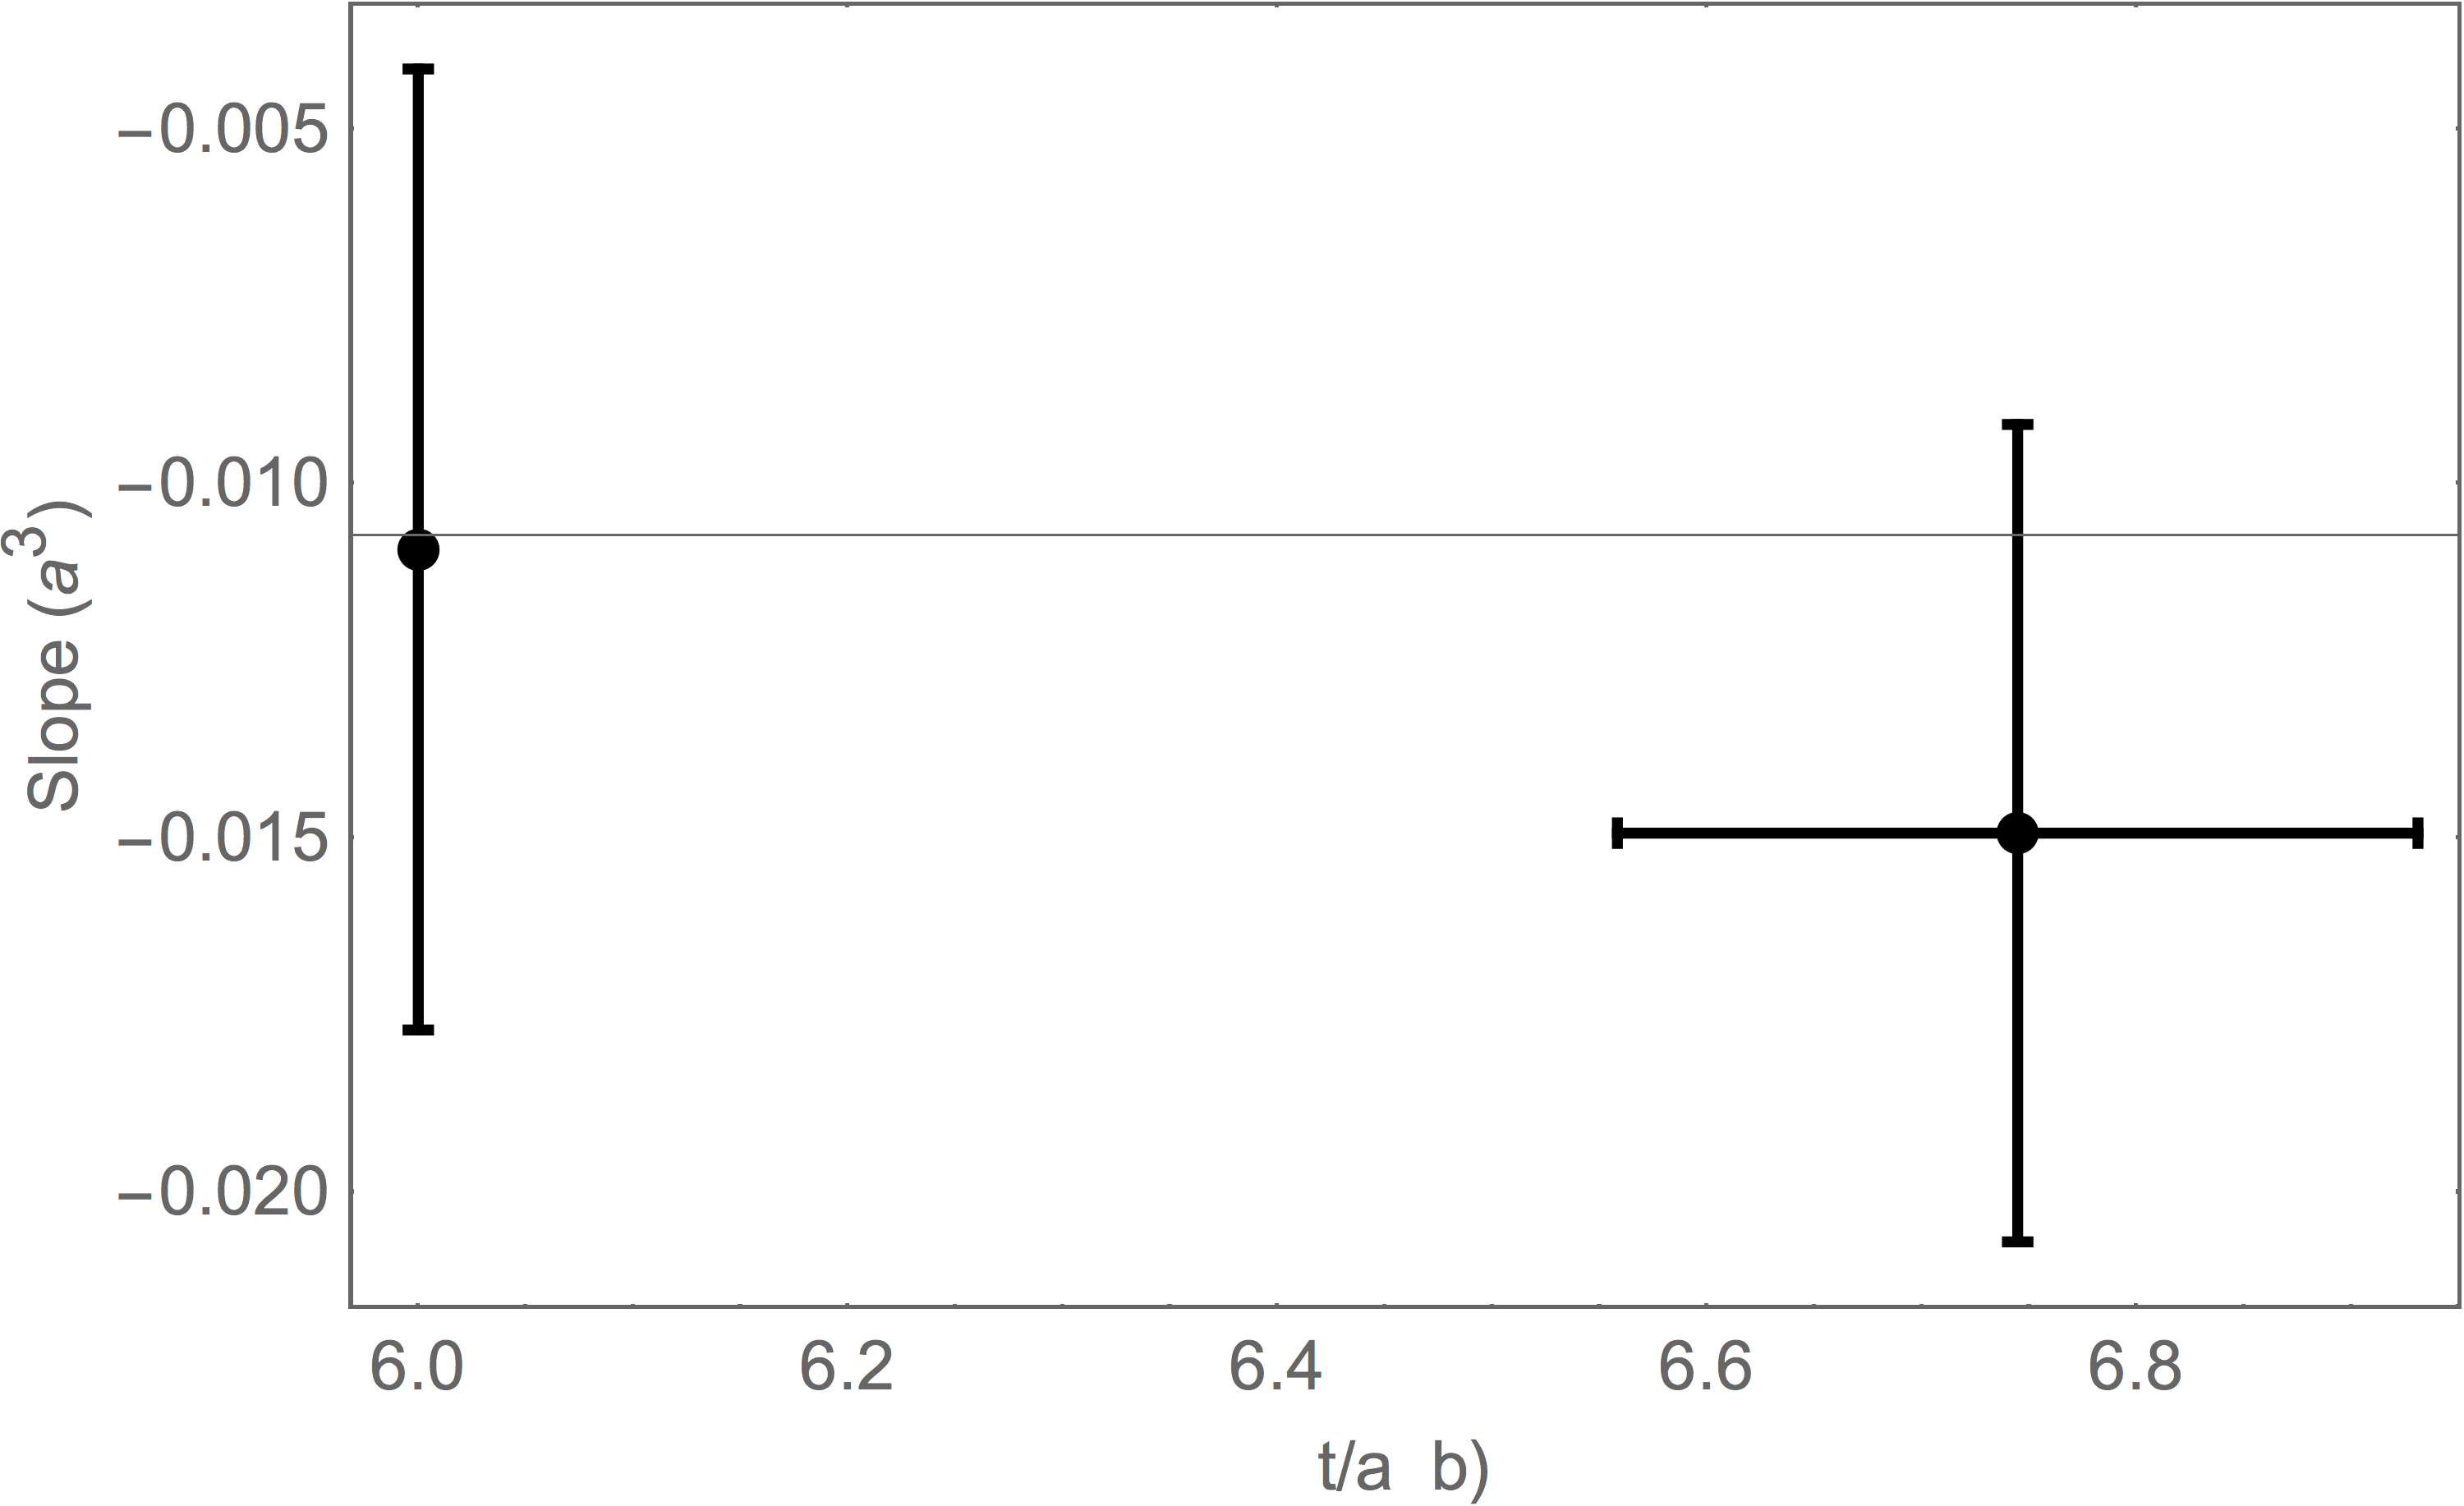
\includegraphics[width=.33\linewidth]{figures/3wC4-8Chi.png}
  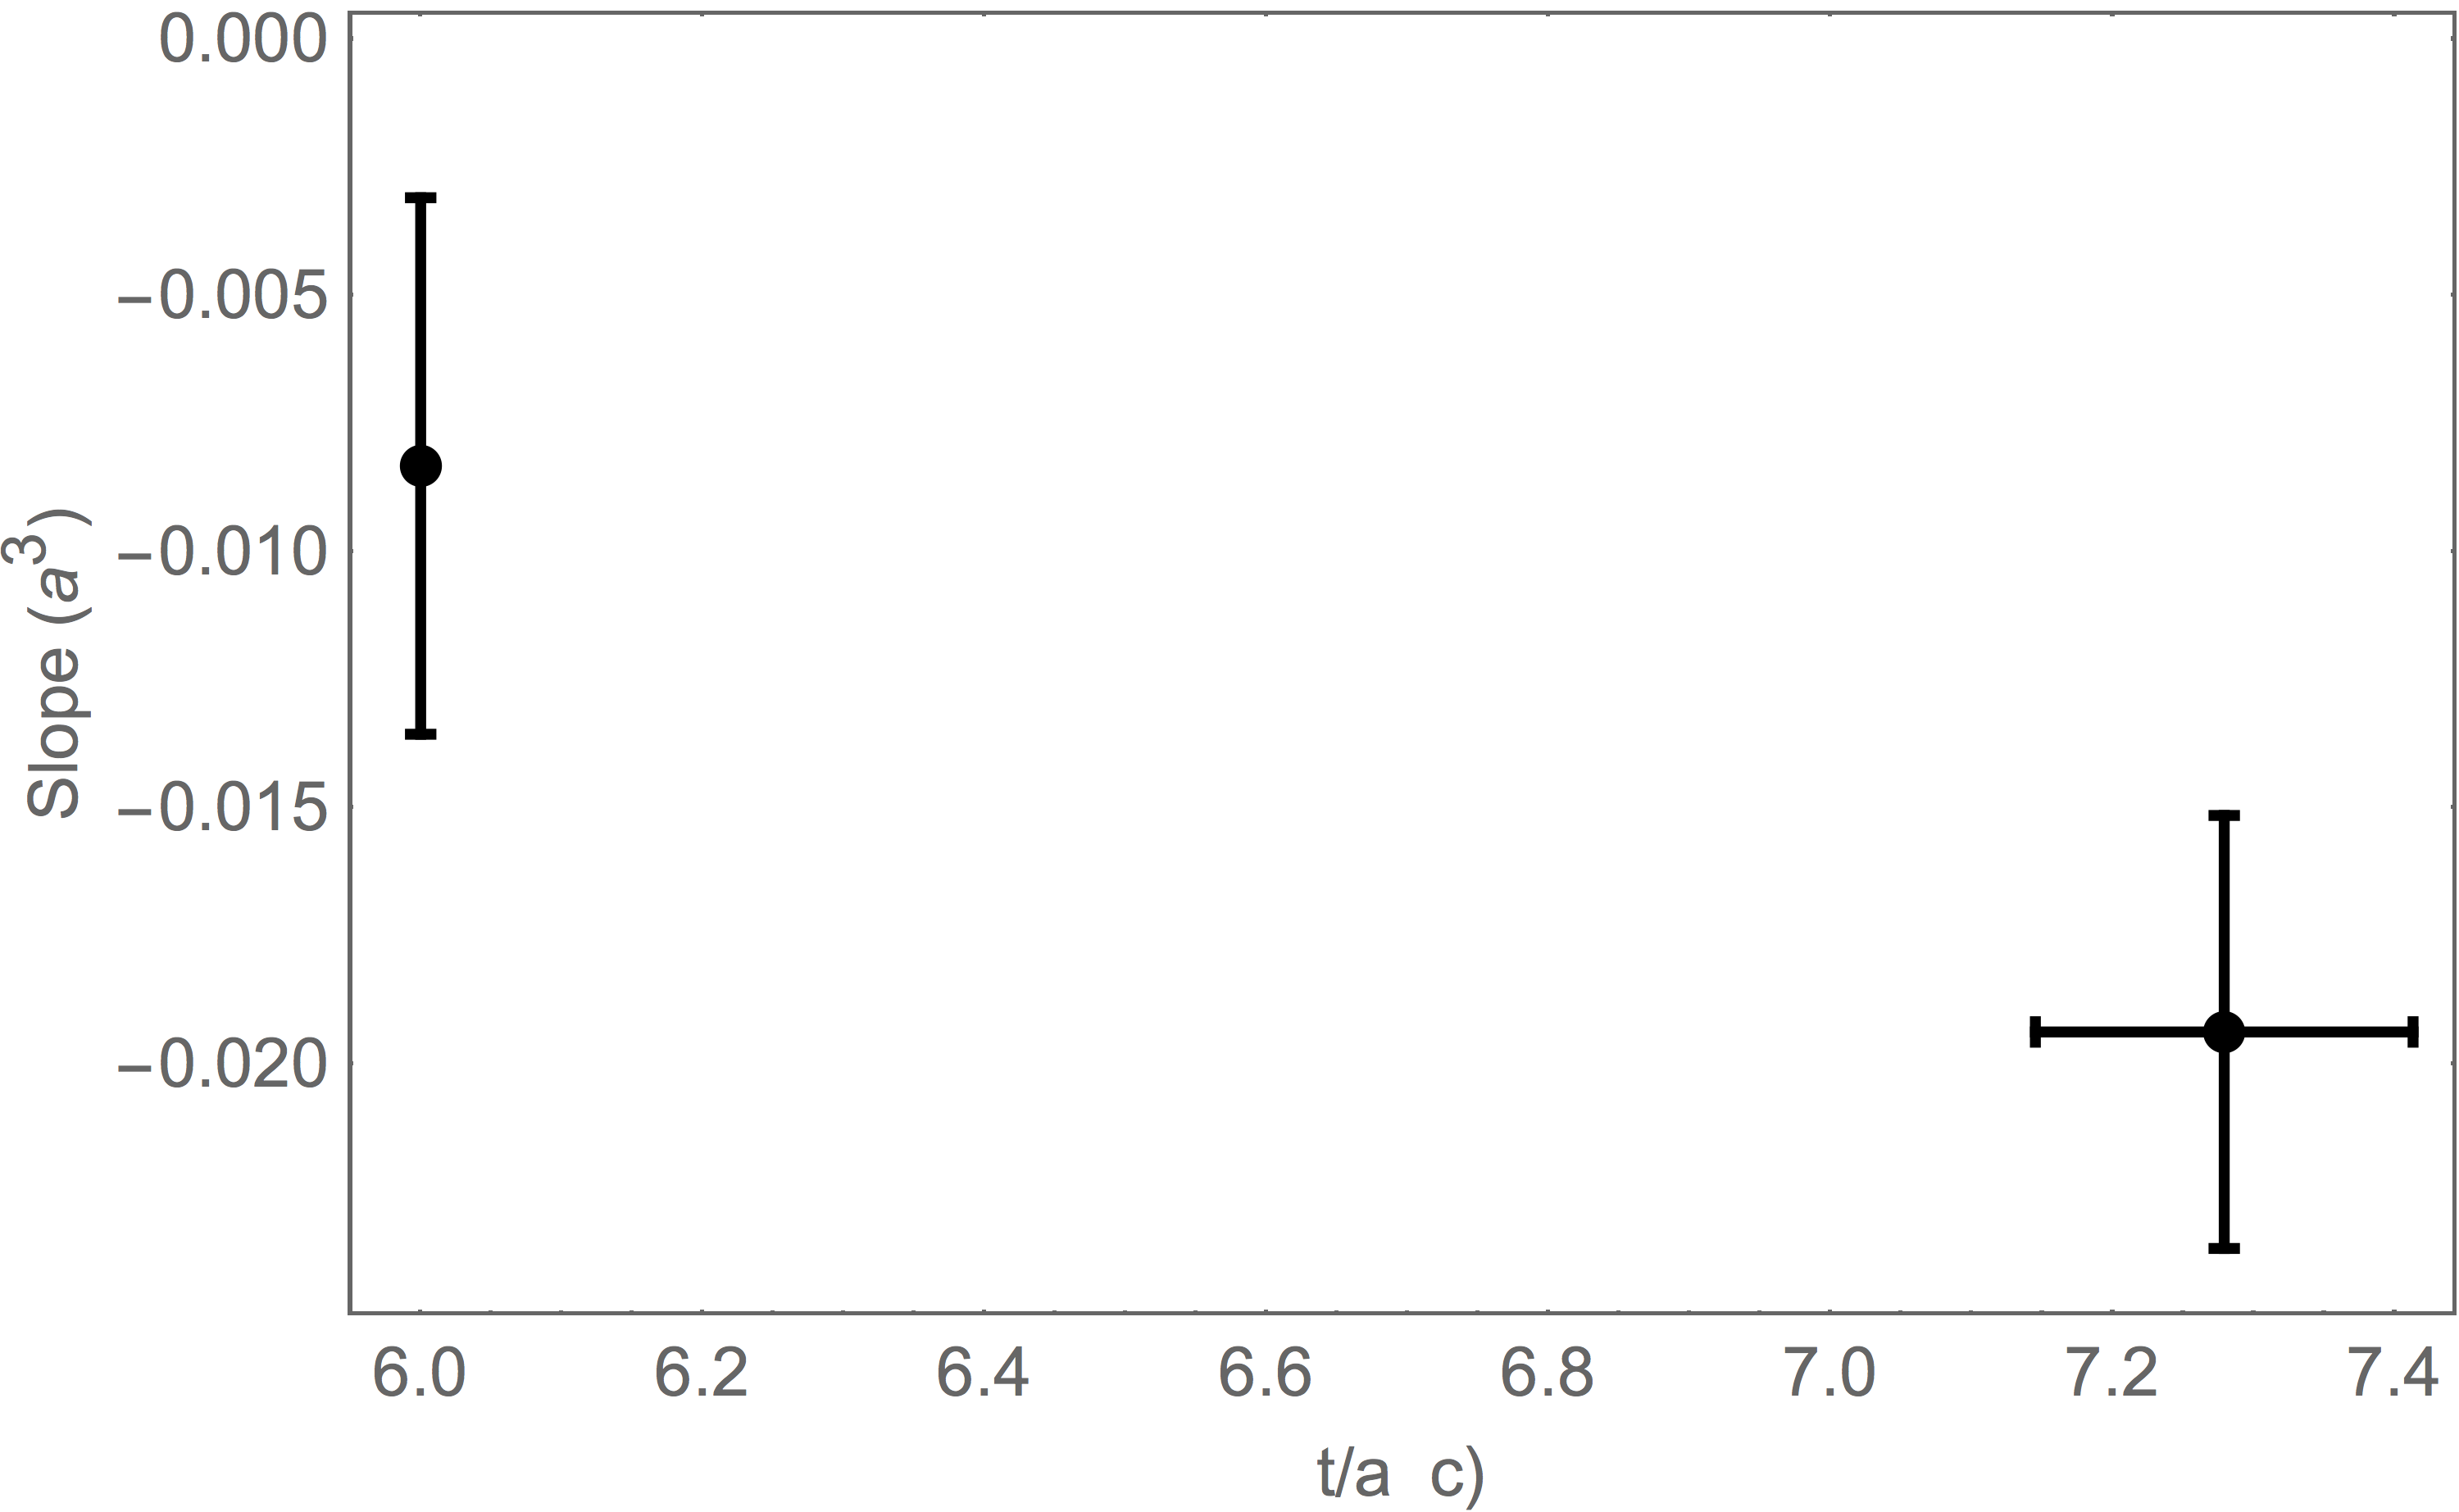
\includegraphics[width=.33\linewidth]{figures/3wC3-9Chi.png}
  \caption{Slope values at the shifted inflection points and at $t=6a$ for the
  connected diagrams. a) 5 to 7, b) 4 to 8, c) 3 to 9 $\chi^2$ fit ranges in the 
  three-window analysis.}
  \label{fig:shifinflecconn}
\end{figure}

Our one-window analysis also confirms that an excited state analysis can be avoided; 
the values of the slopes at the points of inflection also agree within uncertainties.
The results from table~\ref{tab:1walphaconnected} are show in figure~\ref{fig:1wshift_conn}.
\begin{figure}[H]
  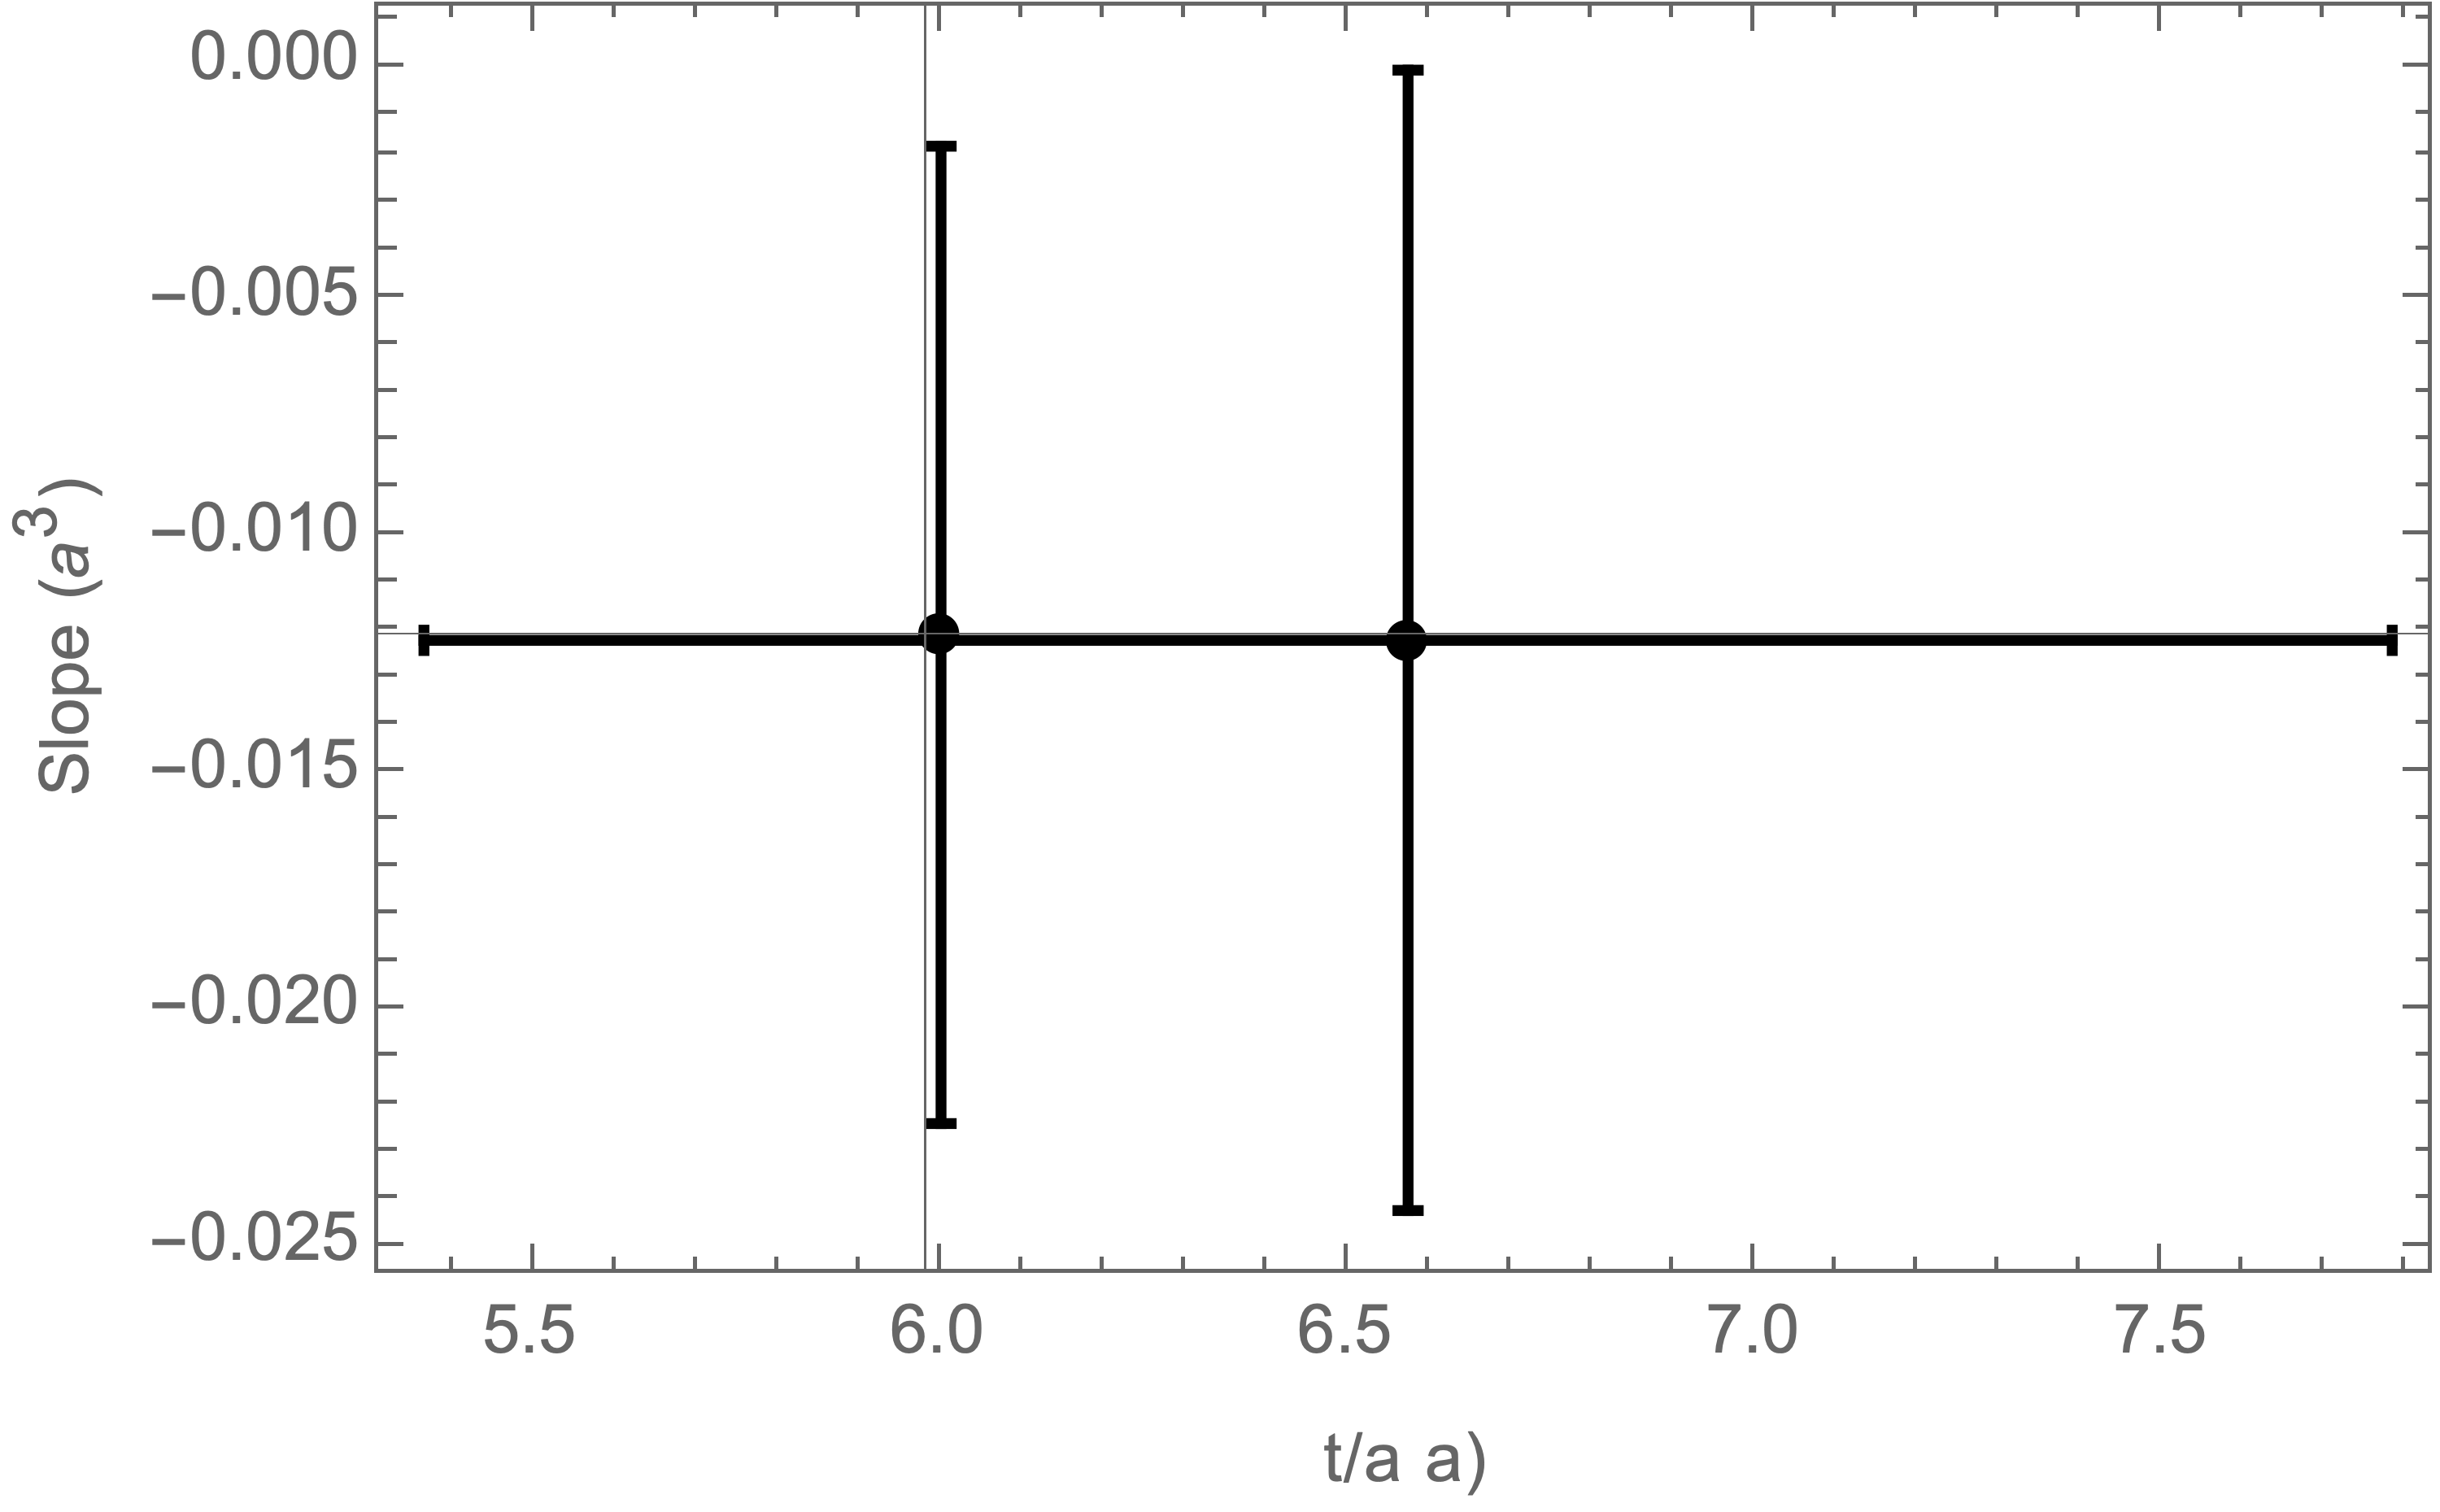
\includegraphics[width=.49\linewidth]{figures/1wC4-8Chi2021.png}
  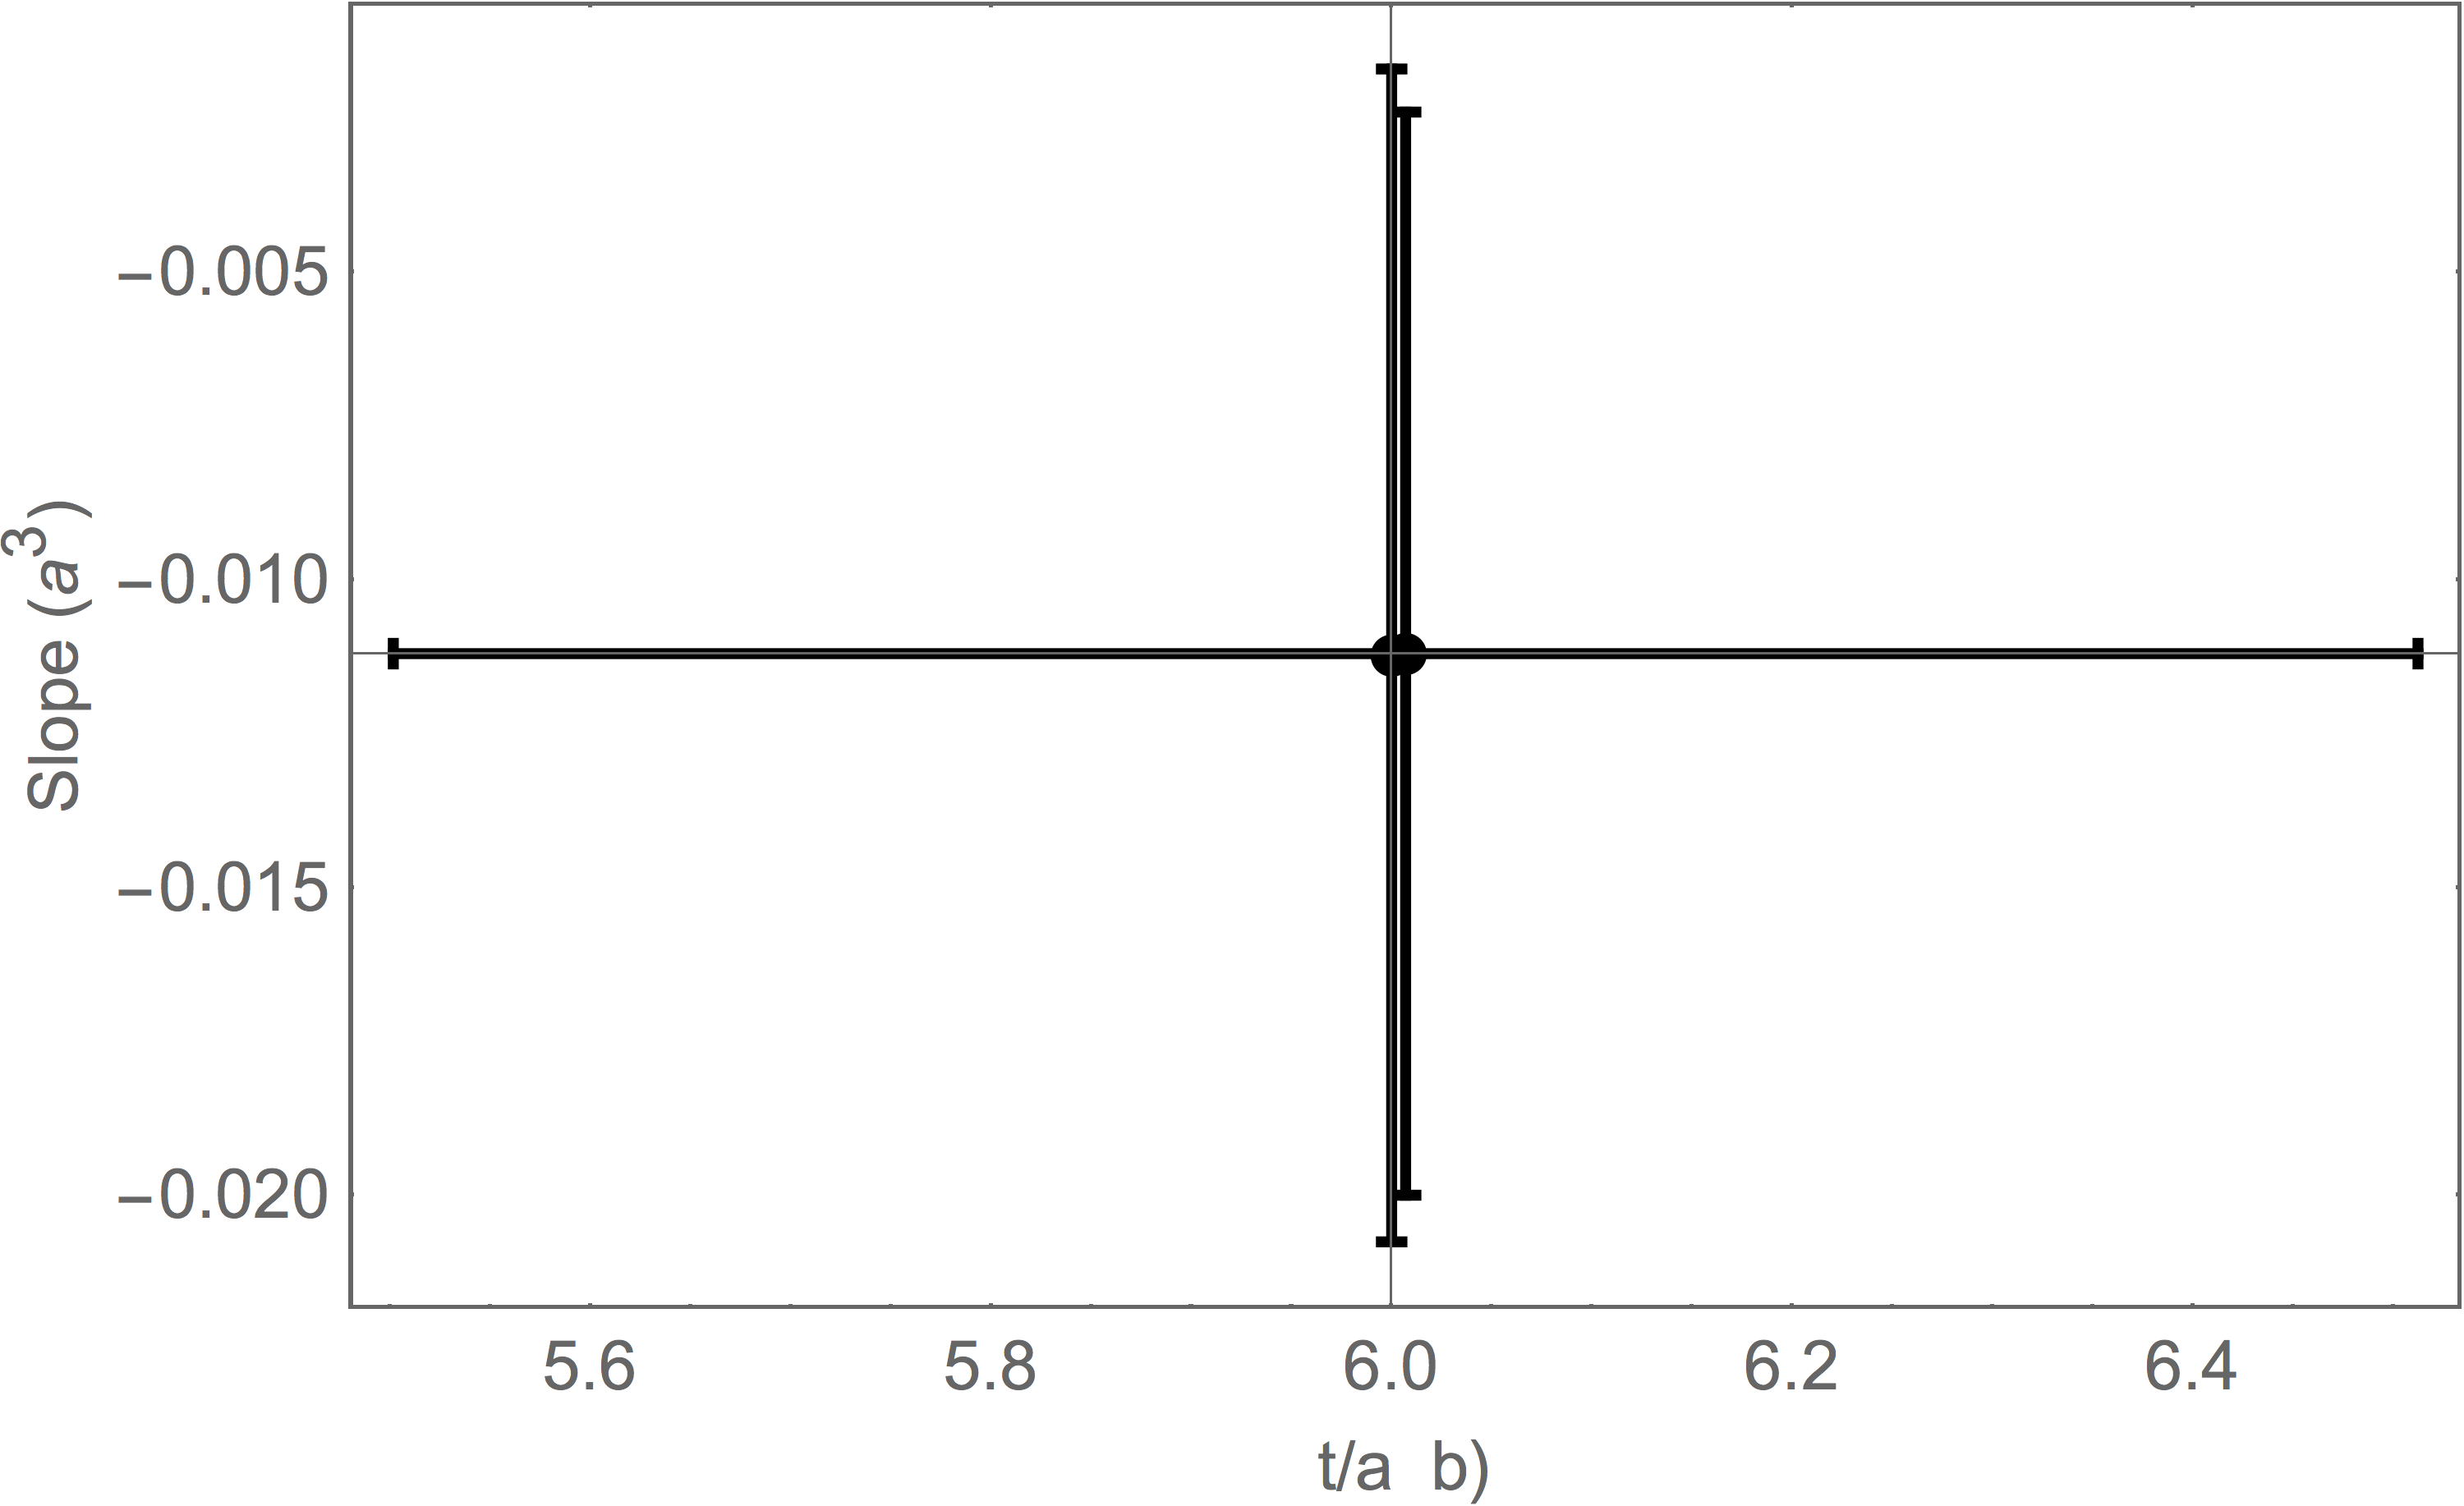
\includegraphics[width=.495\linewidth]{figures/1wC3-9Chi.png}
  \caption{Slope values for the $\chi^2$ fits, with and without a quadratic term. a) 4 to 8,
  b) 3-9 fit ranges for the connected diagrams in the one-window analysis}
  \label{fig:1wshift_conn}
\end{figure}
%%%%%%%%%%%%%%%%%%%%%%
\subsection{Slope values at $t=6a$ for all diagrams in the 3-window and
1-window  analyses}
The slope values at $t=6a$ and at the shifted inflection point also agree within uncertainties, 
as shown in fiigure~\ref{fig:shiftinflec_all}.
%%%% extremal, position and slope, Multi point, All diagrams%%%
\begin{table}[H]
\begin{center}
    \begin{tabular}{ | c | c | c | c |}
    \hline
     Fit range [$t/a$] & 5 to 7    & 4 to 8 & 3 to 9      \\ 
     \hline
   	Inflection point [$t/a$] &   6.99(39)         &      6.97(36)    &    7.12(34)   \\ \hline
        Extremal slope [$a^3$] &    -0.002(24)        &     0.001(19)    &      0.005(16) \\ \hline
 	Slope at $t=6a$ [$a^3$] &    0.010(21)        &     0.010(16)   &     0.016(14)   \\ \hline
    \end{tabular}
\end{center}
\caption{Inflection points, extremal slope and slope at $t=6a$ for the $\chi^2$
linear fits for connected diagrams in the 3-window analysis with parabola minimum lift correction.}
\label{tab:Retardation3wMultiPointAll}
\end{table}
%%%%%%%%%%%%%%
\begin{figure}[H]
  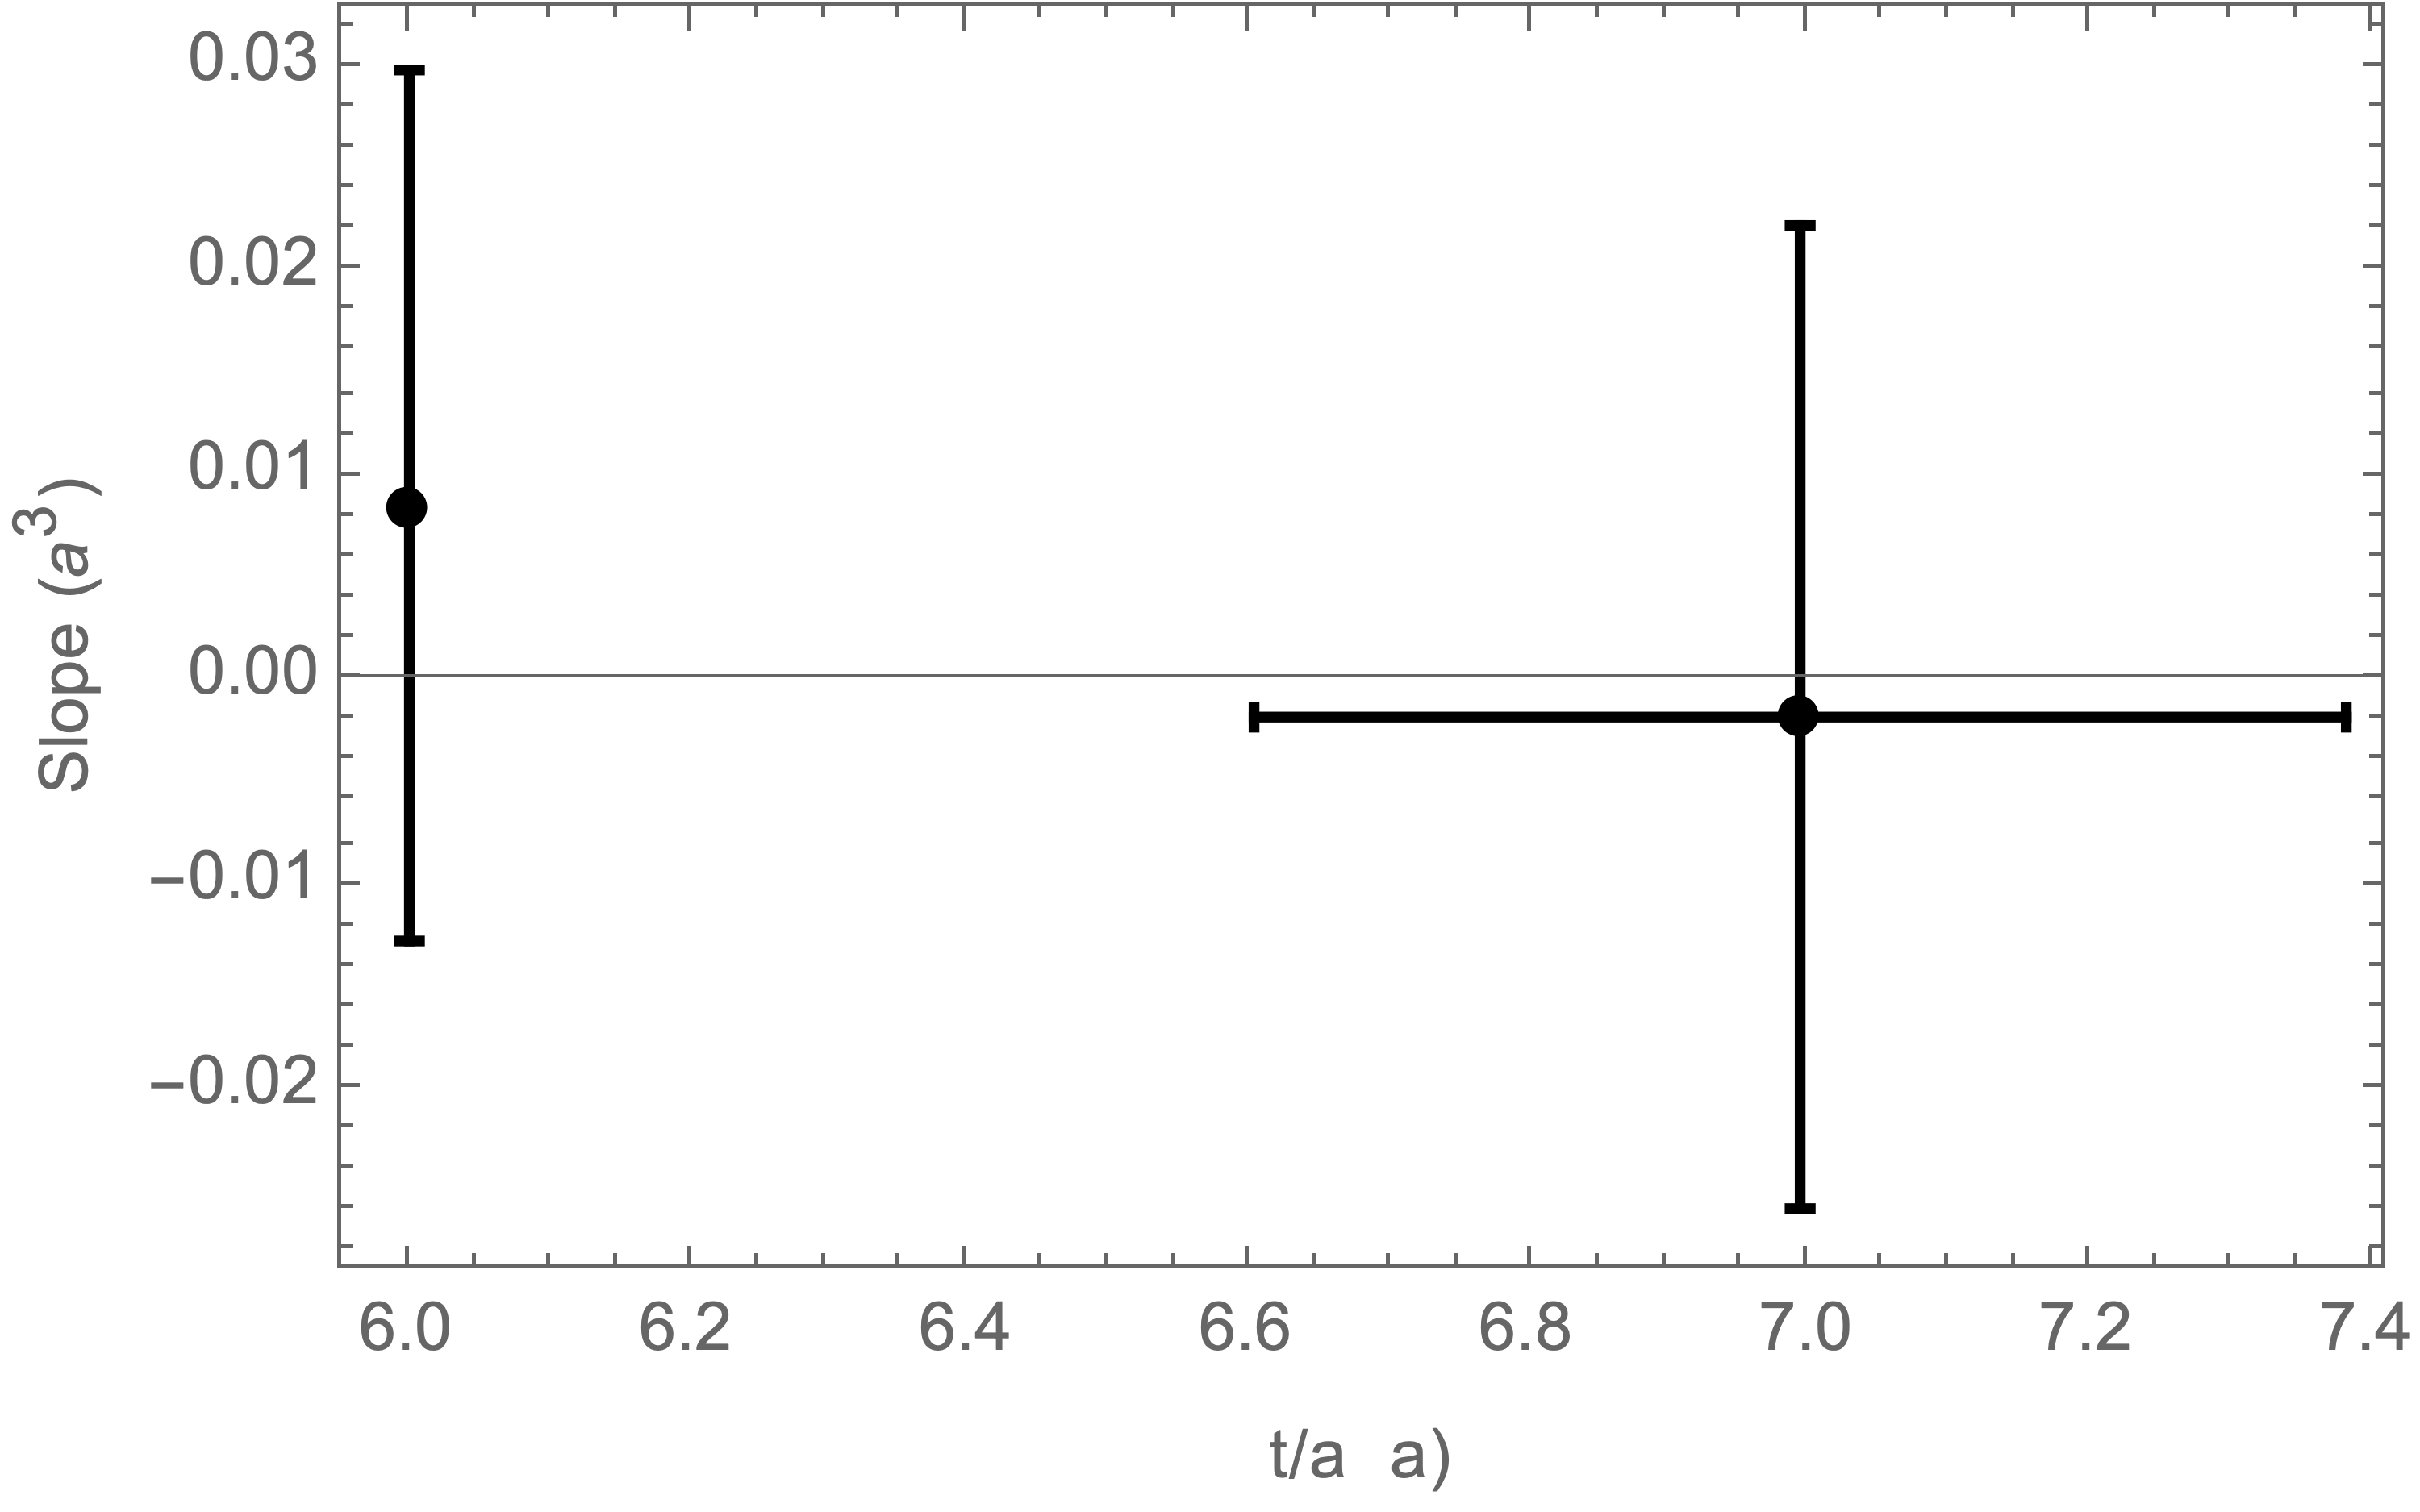
\includegraphics[width=.33\linewidth]{figures/3wF5-7Chi.png}
  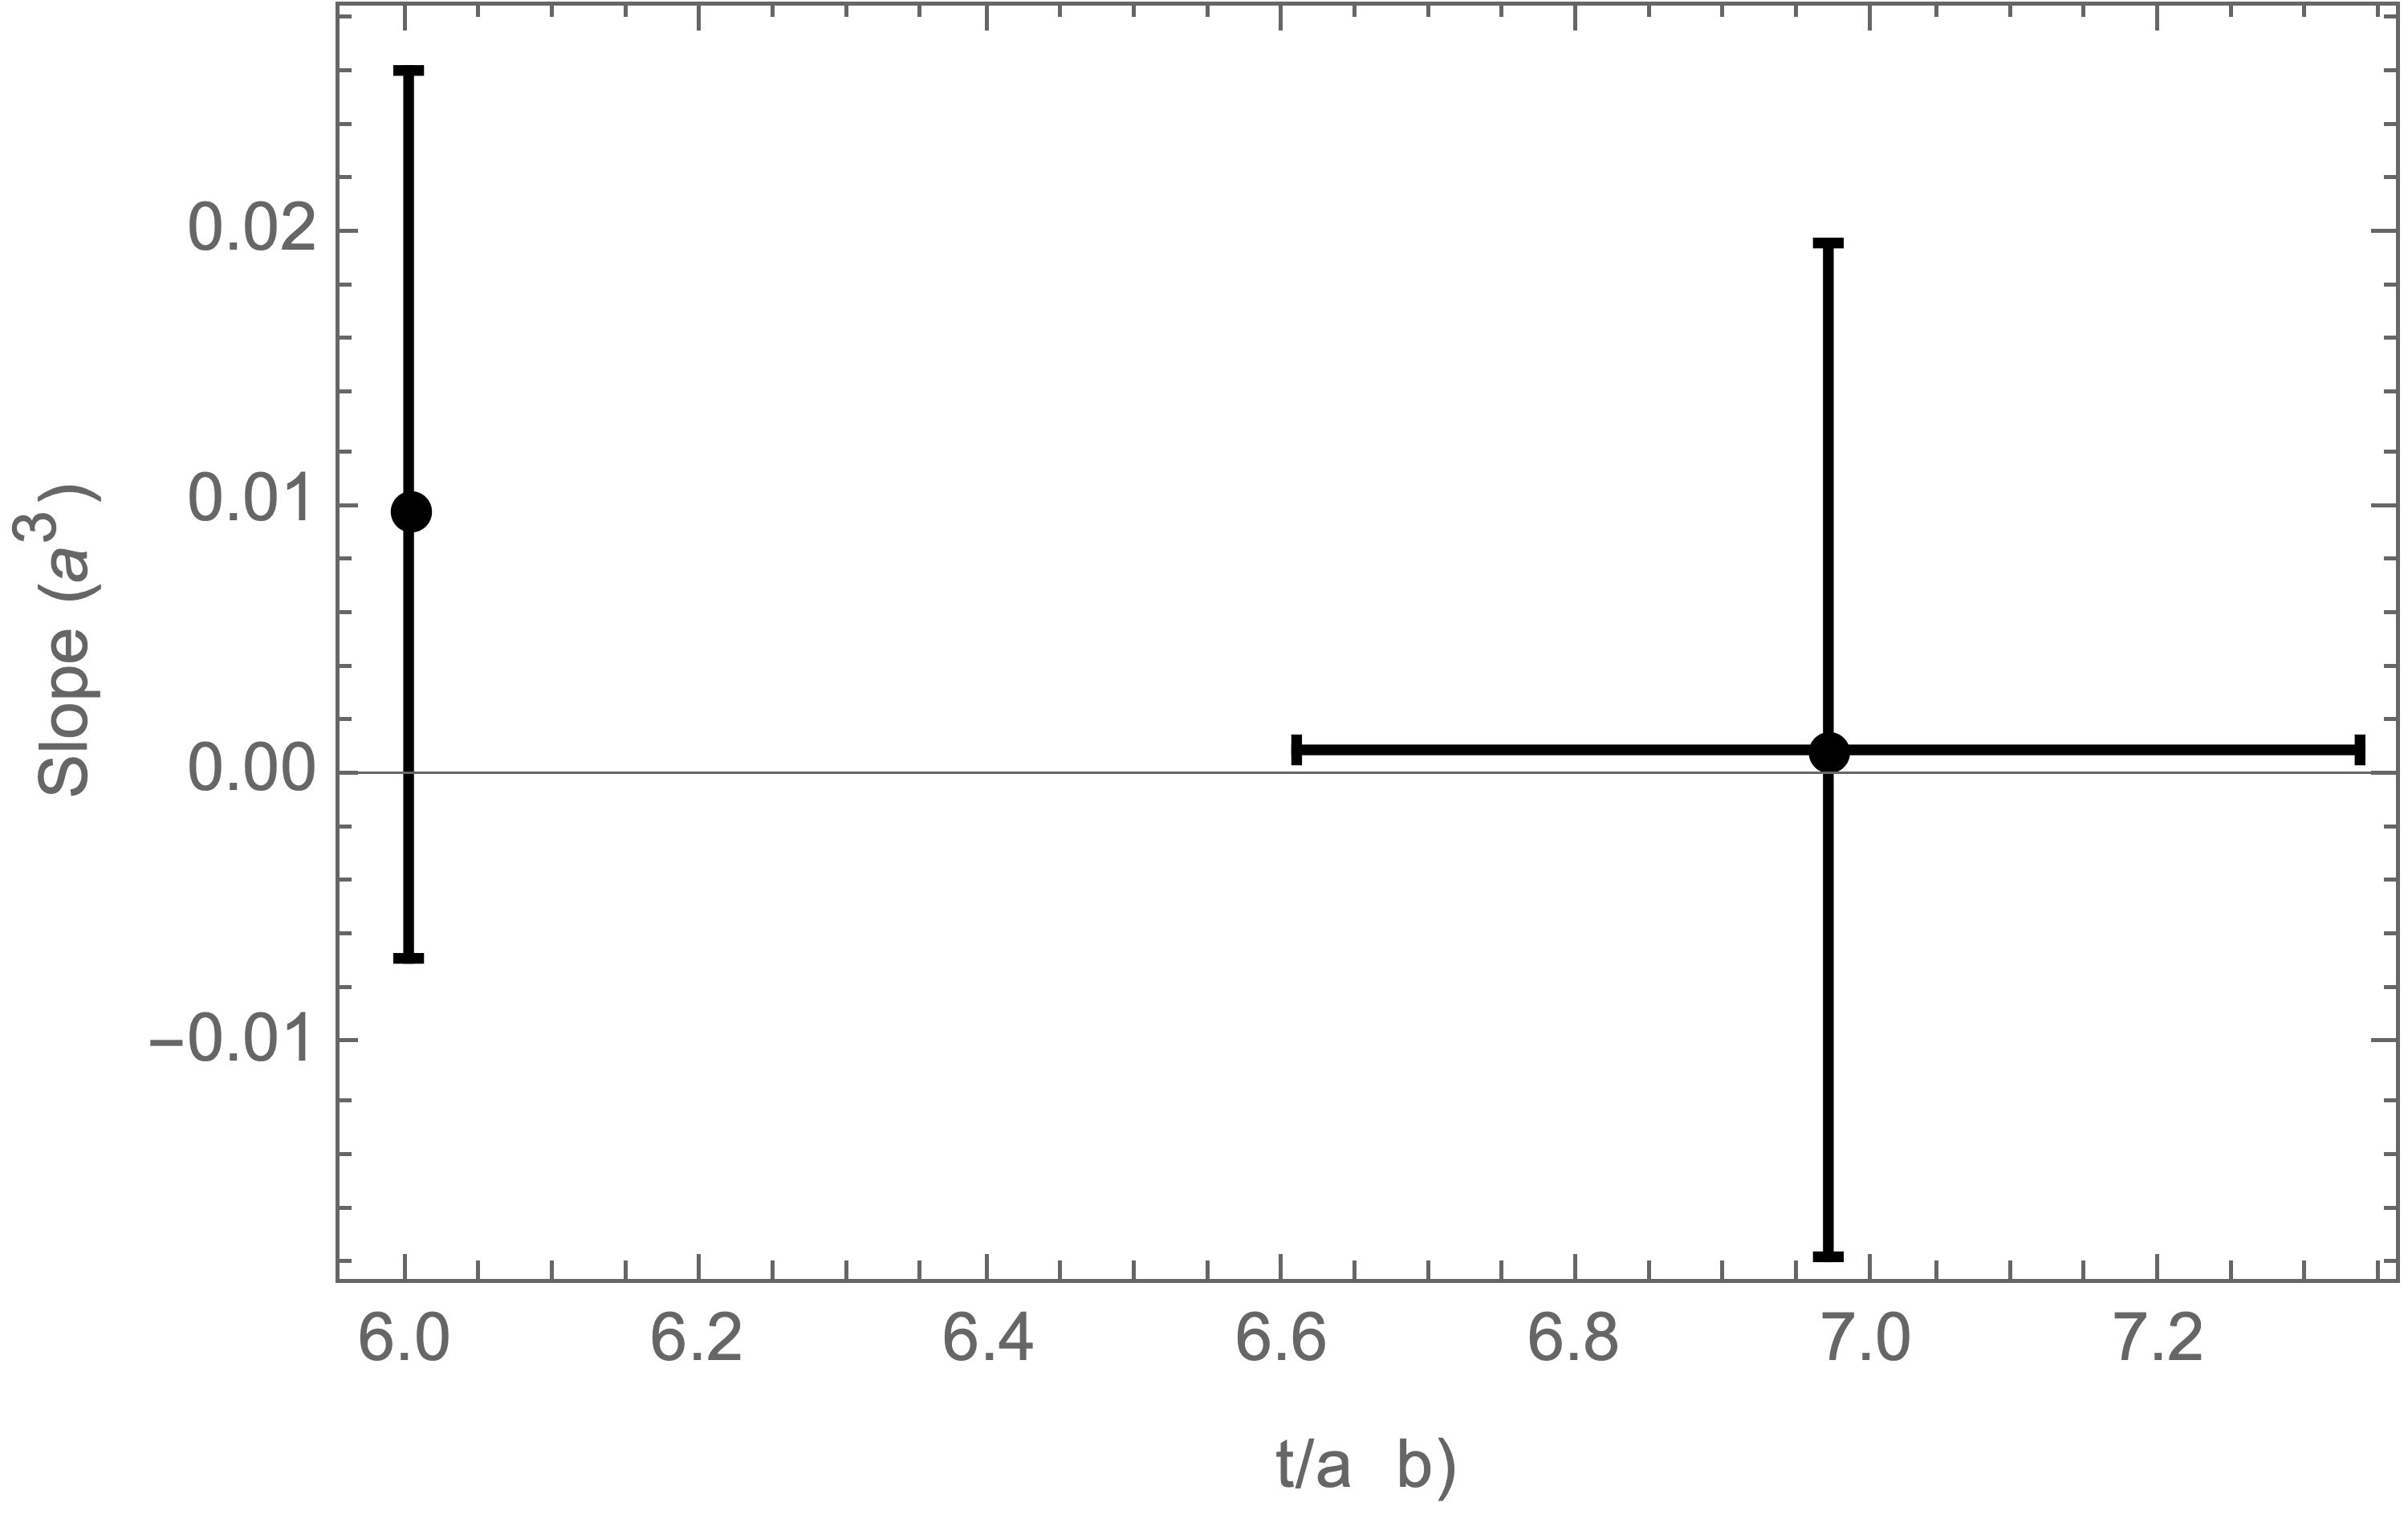
\includegraphics[width=.325\linewidth]{figures/3wF4-8Chi.png}
  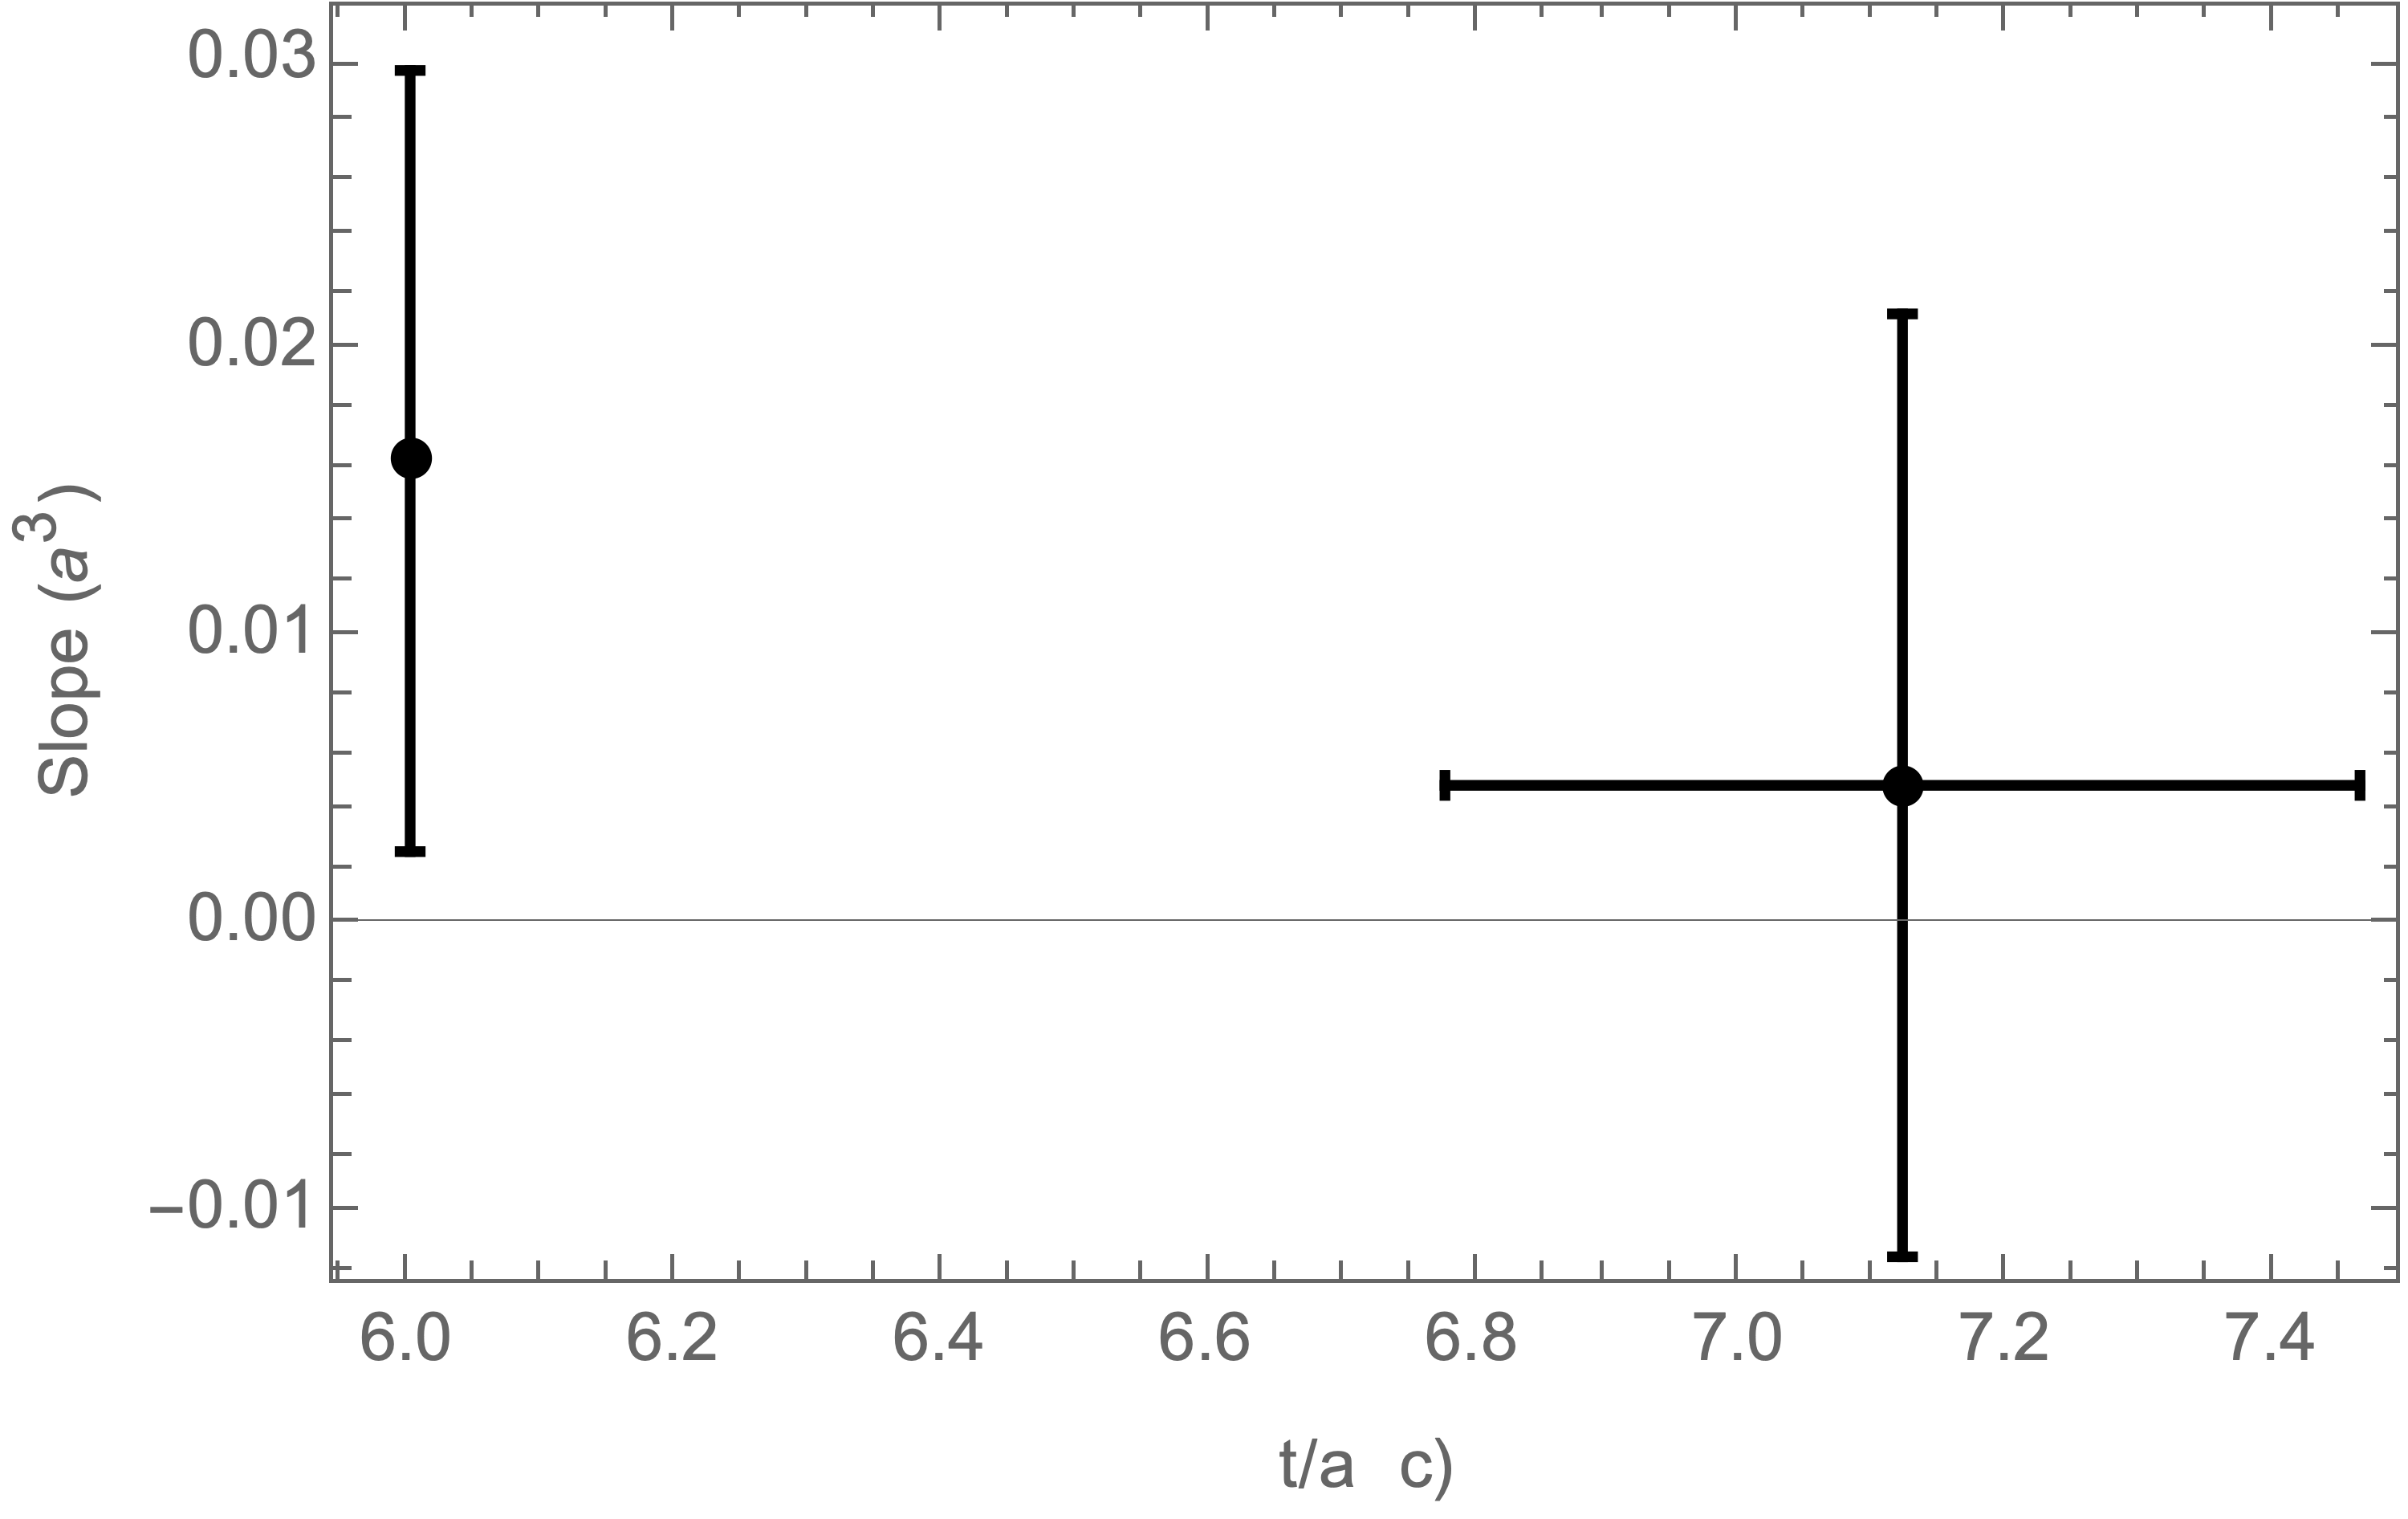
\includegraphics[width=.325\linewidth]{figures/3wF3-9Chi.png}
  \caption{Slope values at the shifted inflection points and at $t=6a$ for all diagrams. a) 5 to 7, 
  b) 4 to 8, c) 3 to 9 $\chi^2$ fitting ranges in the three-window analysis.}
  \label{fig:shiftinflec_all}
\end{figure}
In the $\chi^2$ quadratic fits, in the one-window analysis,  with and without a quadratic terms yield 
positions with a considerable uncertainty. However, the slopes at those points agree within uncertainties 
with those at the inflection point $t=6a$, c.f. table~\ref{tab:1walphaconnected} 
and figure~\ref{fig:1wshifinflec_all}.
\begin{figure}[H]
  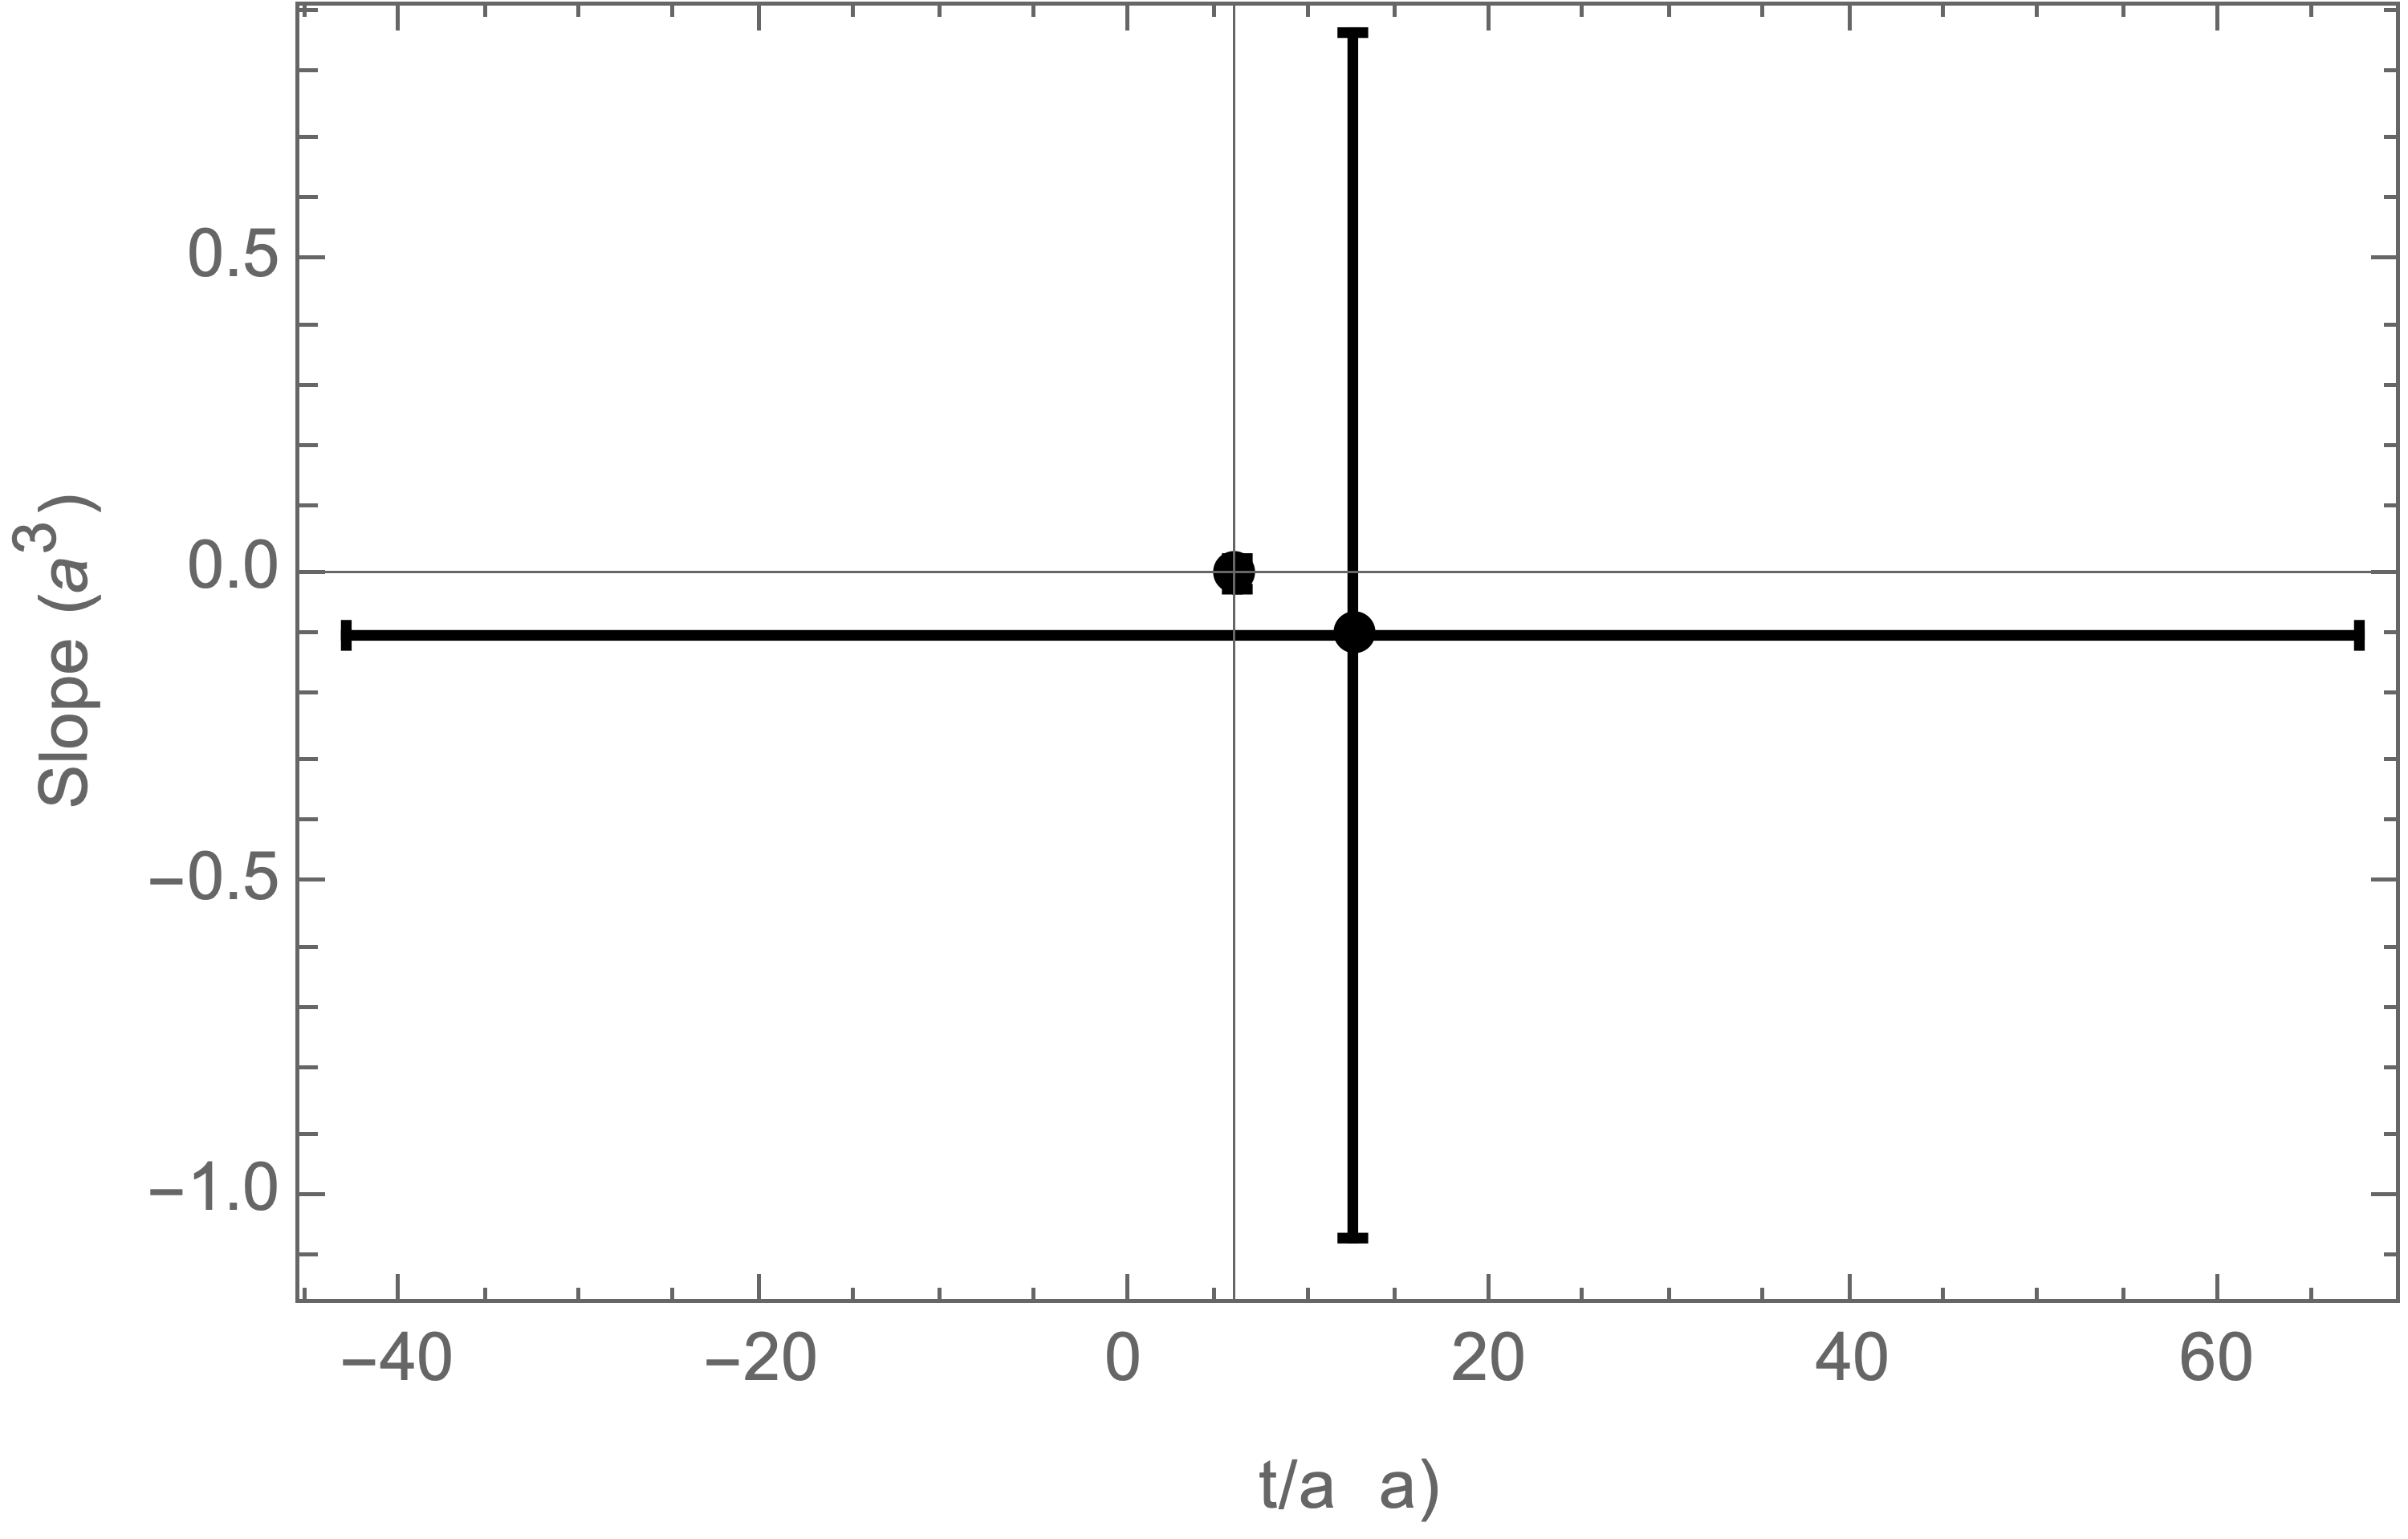
\includegraphics[width=.49\linewidth]{figures/1wF4-8Chi.png}
  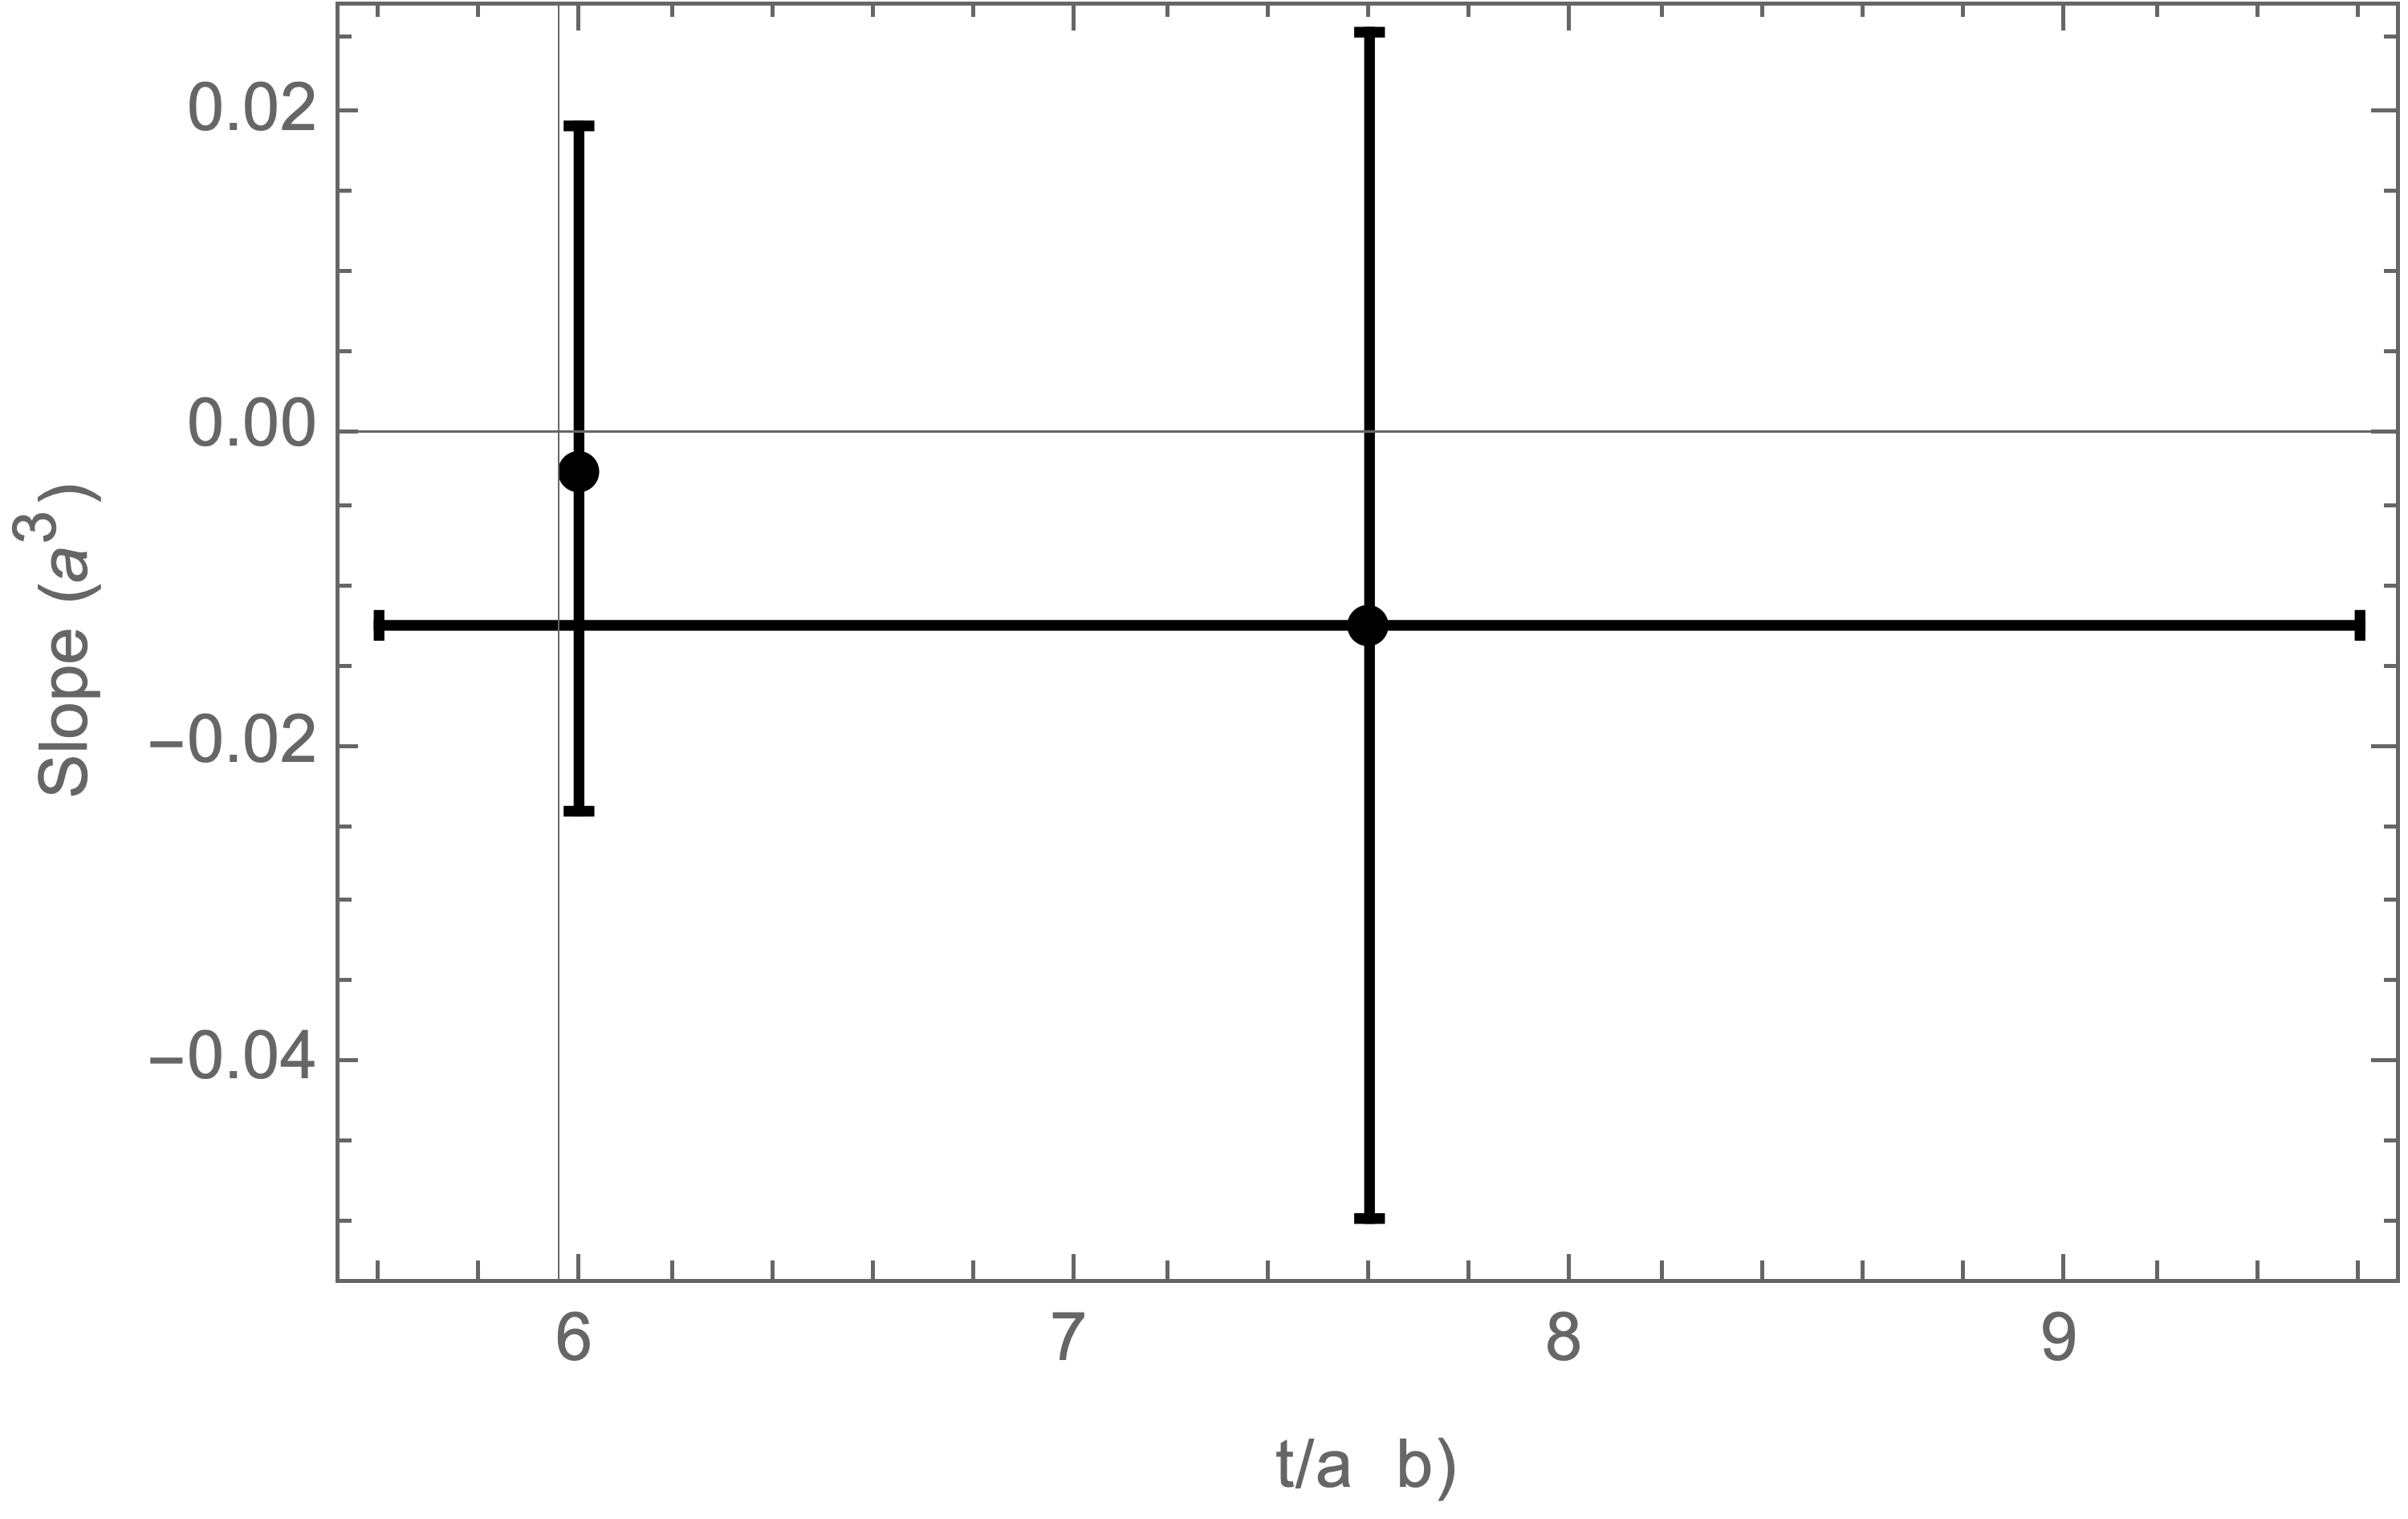
\includegraphics[width=.495\linewidth]{figures/1wF3-9Chi.png}
  \caption{Slope values extracted form the $\chi^2$ fitting ranges a) 4 to 8 and b) 3 to 9 for all diagrams
  in the one-window analysis.}
  \label{fig:1wshifinflec_all}
\end{figure}
The previous connected and all diagrams results show slopes at the inflection point consistent
with the slopes at $t=6a$. Although the 3-window analysis shows that the inflection 
points shift, the one-window analyses yield large uncertainties in their positions. The slopes at 
theses points are also consistent with the ones at the inflection points of construction $t=6a$. 
Consequently, we conclude that our results strongly suggest no excited-state analysis.

\section{Conclusions}

\begin{figure}[H]
\centering
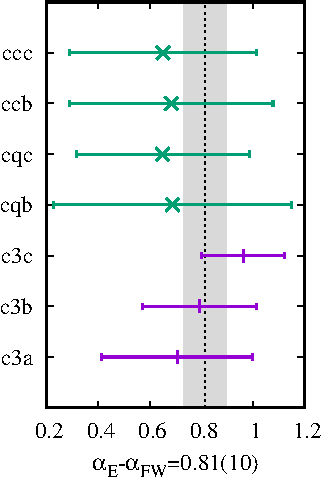
\includegraphics[width=.335\linewidth]{figures/con}
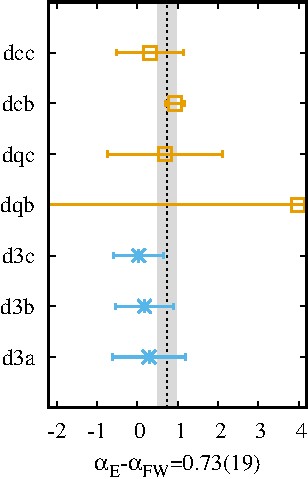
\includegraphics[width=.32\linewidth]{figures/dis}\;\;
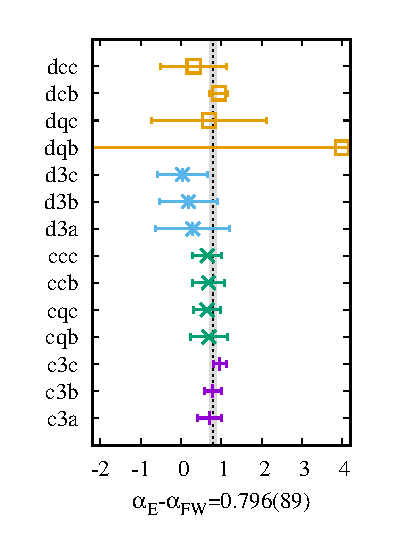
\includegraphics[width=.32\linewidth]{figures/all}
\caption{Various fit results for the electric polarizability $\alpha_E-\alpha_{FW}$, 3-letter fit label: 1) connected (c) + disconnected (d) data; 2) 3-window fit (3), 1-window fit with (q) or without (c) quadratic term; 3) fit range 5 to 7 (a), 4 to 8 (b) and 3 to 9 (c) including corresponding (simple) averages in the abscissa labels (not taking into account correlations!).}
\label{fig:Correlators3wAll}
\end{figure}



\section*{Acknowledgments}
Fruitful discussions with S.~A.~Coon, W.~Detmold, H.~Grie\ss hammer and B.~Pasquini are acknowledged.
This research was supported by the Erwin Schr\"odinger Fellowship program of the Austrian Science Fund FWF (``Fonds zur F\"orderung der wissenschaftlichen Forschung'') under Contract No. J3425-N27 (R.H.) and the U.S.~Department of Energy, Office of Science, Office of Nuclear Physics through grant DE-FG02-96ER40965 (M.E.,J.S.).



\bibliographystyle{utphys} % We choose the &quot;plain&quot; reference style
\bibliography{main}

\end{document}


\section*{References}
\begin{thebibliography}{99}
\bibitem{babusci} D.~Babusci, G.~Giordano, A.~I.~L'avov, G.~Matone, A.~M.~ Nathan, Phys.~Rev.~C {\bf{58}}, 1013,1041 (1998), arXiv: hep-ph/9803347.
\bibitem{hagelstein} F.~Hagelstein, Symm.~ {\bf{12}}, 1407 (2020).
\bibitem{levchuk} M.~I.~ Levchuk, A.~I.~L'vov, Nucl.~Phys.~{\bf{A674}}, 449 (2020).
\bibitem{bernard1} V.~Bernard, N.~Kaiser, U.~Meissner, Phys.~Rev.~Lett.~ {\bf{67}}, 1515 (1991).
\bibitem{bernard2} V.~Bernard, N.~Kaiser, U.~Meissner, Nucl.~Phys.~{\bf{B373}}, (1992)
\bibitem{detmold} W.~Detmold, B.~C.~Tiburzi, A.~Walker-Loud, Phys. Rev. D {\bf{73}}, 114505 (2006).
\bibitem{schumacher} M.~Schumacher, LHEP {\bf{2}}, 4 (2019).
\bibitem{foldywouthuysen} J.~Saenz, M.~Engelhardt, R.~H\"ollwieser,
Phys. Rev. D. {\bf 104}, 056002 (2021).
\bibitem{holstein} B.~Holstein, D.~Drechsel, B.~Pasquini, and M.~Vanderhaeghen, Phys.~Rev.~C {\bf{61}}, 034316 (2000).
\bibitem{drechsel} D.~Dreschsel, B.~Pasquini, and M.~Vanderhaeghen, Phys.~Rep.~{\bf{378}}, 99 (2003).
\bibitem{hildebrandt} R.~Hildebrandt, H.~Grie{\ss}hammer, T.~Hemmert, and B.~Pasquini, Eur.~Phys.~J.~ A {\bf{20}}, 293 (2004).
\bibitem{schumacher2} M.~Schumacher, Porg.~Part.~Nucl.~Phys.~{\bf{55}}, 567 (2005).
\bibitem{pasquini1} B.~Pasquini, D.~Drechsel, and M.~Vanderhaeghen, Phys.~Rev.~C {\bf{76}}, 015203 (2007).
\bibitem{pasquini2} B.~Pasquini, P.~Pedroni, adn D.~Drechsel, Phys.~Lett.~ B {\bf{687}}, 160 (2010).
\bibitem{griesshammer2} H.~Grie{\ss}hammer, J.~McGovern, D.~R.~Phillips, and G.~Feldman, Prog.~Part.~Nucl.~Phys.~{\bf{67}}, 841 (2012).
\bibitem{mcgovern} J.~McGovern, D.~R.~Phillips, and H.~Grie{\ss}hammer, Eur.~Phys.~J.~A {\bf{49}}, 12 (2013).
\bibitem{holstein2} B.~Holstein adn S.~Scherer, Annu.~Rev.~Nucl.~Part.~Sci.~{\bf{64}}, 51 (2014).
\bibitem{myers} L.~S.~Myers {\it{et al.}} (COMPTON@MAX-lab Collaboration), Phys.~Rev.~Lett.~{\bf{113}}, 262506 (2014).
\bibitem{martel} P.~Martel {\it{et al.}} (A2 Collaboration), Phys.~Rev.~Lett.~{\bf{114}}, 112501 (2015).
\bibitem{gryniuk} O.~Gryniuk, F.Hagelstein, and V.~Pascalutsa, Phys.~Rev.~D {\bf{92}}, 074031 (2015).
\bibitem{gryniuk2} O.~Gryniuk, F.~Hagelstein, abd V.~Pascalutsa, Phys.~Rev.~D {\bf{94}}, 034043 (2016).
\bibitem{hagelstein2} F.Hagelstein, R.~Miskimen, and V.~Pascalutsa, Prog.~Part.~Nucl.~Phys.~{\bf{88}}, 29 (2016).
\bibitem{griesshammer3} H.~Grie{\ss}hammer, J.~McGovern, and D.R.~Phillips, Eur.~Phys.~J.~A {\bf{54}}, 37 (2018).
\bibitem{pasquini3} B.~Pasquini, P.~Pedroni, and S.~Sconfietti, Phys.~Rev.~C {\bf{98}}, 015204 (2018).
\bibitem{pasquini4} B.~Pasquini and M.~Vanderhaeghen, Annu.~Rev.~Nucl.~Part.~Sci.~{\bf{68}}, 75 (2018).
\bibitem{pasquini5} B.~Pasquini, P.~Pedroni, and S.~Sconfietti, J.~Phys.~G {\bf{46}}, 104001 (2019).
\bibitem{miskimen} R.~Miskimen, Proc.~Sci., CD2018 ({\bf{2019}}) 015.
\bibitem{martel2} P.~Martel {\it{et al.}} (A2 Collaboration), Porc.~Sic., CD2018 ({\bf{2019}}) 038.
\bibitem{paudyal} D.~Paudyal {\it{et al.}} (A2 Collaboration), Phys.~Rev.~C {\bf{102}}, 035205 (2020).
\bibitem{melendez} J.~Melendez, R.~Furnstahl, H.~Grie{\ss}hammer, J.~McGovern, D.~R.~Phillips, and M.~Patrola, Eur.~Phys.~J.~A {\bf{57}}, 81 (2021).

\bibitem{fiebig} H.~Fiebig, W.~Wilcox, R.~M.~Woloshyn, Nucl. Phys. {\bf{B324}}, 47 (1989).
\bibitem{christensen2} J.~Christensen, W.~Wilcox, F.~X.~Lee, K.~Zhou, Phys. Rev. {\bf{72}}, 034503 (2005).
\bibitem{lee} F.~X.~Lee, L.~Zhouz, W.Wilcox, J.~Christensen, Phys. Rev D{\bf{73}},  034503 (2006).
\bibitem{shintani} E.~Shintani, S.~Aoki, N.~Ishizuka, K.~Kanaya, Y. Kikukawa, Y.~Kuramashi,
M.~Okawa, A.~Ukawa, and T.~Yoshie, Phys.~Rev.~D {\bf{75}}, 034507 (2007).
\bibitem{engelhardt1} M.~Engelhardt, Phys. Rev. D {\bf{76}}, 114502 (2007).
\bibitem{engelhardt2} M.~Engelhardt, Proc. Sci. LAT2009 ({\bf{2009}}) 128.
\bibitem{detmold2} W.~Detmold, B.~Tiburzi, and A.~Walker-Loud, Phys.~Rev.~D {\bf{79}}, 094505 (2009).
\bibitem{detmold3} W.~Detmodl, B.~Tiburzi, and A.~Walker-Loud, Phys.~Rev.~D {\bf{81}}, 054502 (2010).
\bibitem{engelhardt3} M.~Engelhardt, Proc. Sci. Lattice 2011 ({\bf{2011}}) 153.
\bibitem{alexandru} A.~Alexandru and F.~X.~Lee, Proc. Sci. LAT2009 ({\bf{2009}}) 144.
\bibitem{lee1} F.~X.~ Lee and A. Alexandru, Proc.~Sci., Lattice 2010 ({\bf{2010}}) 148.
\bibitem{lee3} F.~X.~ Lee and A.~Alexandru, Proc.~Sci., Lattice 2011 ({\bf{2011}}) 317.
\bibitem{lujan} M.~Lujan, A.~Alexandru, W.~Freeman, and F.~X.~Lee, Phys.~Rev.~D {\bf{89}}, 074506 (2014).
\bibitem{freeman} W.~Freeman, A.~Alexandru, M.~Lujan, adn F.~X.~Lee, Phys.~Rev.~D {\bf{90}}, 054507 (2014).
\bibitem{luschevskaya} E.~V.~Luschevskaya, O.~E.~Solovjeva, O.~A.~Kochetkov, and O.~V.~Teryaev, Nucl.~Phys.~{\bf{B898}},
627 (2015).
\bibitem{lujan2} M.~Lujan, A.~Alexandru, W.~Freeman, and F.~X.~Lee, Phys.~Rev.~D {\bf{94}}, 074506 (2016).
\bibitem{primer} T.~Primer, W.~Kamleh, D.~Leinweber, and M.~Burkardt, Phys.~Rev.~D {\bf{89}}, 034508 (2014).
\bibitem{bignell} R.~Bignell, J.~Hall, W.~Kamleh, D.~Leinweber, and M.~Burkardt, Phys.~Rev.~D {\bf{98}}, 034504 (2018).
\bibitem{bignell2} R.~Bignell, W.~Kamleh, and D.~Leinweber, Phys.~Rev.~D {\bf{101}}, 094502 (2020).
\bibitem{bignell3} R.~Bignell, W.~Kamleh, adn D.~Leinweber, Phys.~Lett.~B {\bf{811}}, 135853 (2020).
\bibitem{he} F.~He, D.~Leinweber, A.~Thomas, adn P.~Wang, Phys.~Rev.~D {\bf{102}}, 114509 (2020).
\bibitem{bignell4} R.~Bignell, W.~Kamleh, and D.~Leinweber, EPJ WEb Conf. {\bf{245}}, 06033 (2020).

\bibitem{lensky} V.~Lensky, J.~McGovern, and V.~Pascalutsa, Eur.~Phys.J.~C {\bf{75}}, 604 (2015).
\bibitem{griesshammer} H.~Griesshammer, J.~McGovern, and D.~R.Phillips, Eur.~Phys.~J.~A {\bf{52}}, 139 (2016).
\bibitem{jwlee1} J.-W.~Lee and B.~Tiburzi, Phys.~Rev.~D {\bf{89}}, 054017 (2014).
\bibitem{jwlee2} J.-W.~Lee and B.~Tiburzi, Phys.~Rev.~D {\bf{90}}, 074036 (2014).
\bibitem{wilcox1} W.~Wilcox, Ann. Phys. {\bf{255}}, 60 (1997).
\bibitem{wilcox2} W.~Wilcox, Phys. Rev D {\bf{57}}, 6731 (1998).
\bibitem{christensen} F.~X.~Lee, W.~Wilcox, L.~Zhou, Nucl. Phys.~Proc.~Suppl. {\bf{119}}, 269 (2003).

\bibitem{zhou} L.~Zhou, F.~X.~Lee, W.~Wilcox, J.~Christensen, Nucl. Phys. Porc. Suppl. {\bf{119}}, 272 (2003).
\bibitem{lee2} F.~X.~Lee, L.~Zhou, W.~Wilcox, J.~Christensen, PoS {\bf{LAT2005}}, 031 (2006).
\bibitem{MILC} C.~W. Bernard, T.~Burch, K.~Orginos, D.~Toussaint, T.~A.~DeGrand, C.~DeTar, S.~Datta,
S.~A.~Gottlieb, U.~M.~Heller adn R.~Sugar, Phys.~Tev.~\textbf{D 64} (2001) 054506.
\bibitem{foldy} L.~Foldy, Phys. Rev. Lett. {\bf 3}, 105 (1959).
\bibitem{engelhardt4} S.~N.~Syritsyn, J.~D.~Bratt, M.~F.~Lin, H.~B.~Meyer, J.~W.~Negele, A.~V.~Pochinsky, M.~Procura, M.~Engelhardt, Ph.~Hagler, T.~R.~Hemmert, W.~Schroers, Phys.~Rev.~D {\bf 81}, 034507 (2010).
\bibitem{PDG2017} C.~Patrignani et al. (Particle Data Group), Chin. Phys. C, {\bf 40}, 100001 (2016) and 2017 update.
\bibitem{bratt} J.~D.~Bratt, R.~G.~ Edwards, M.~Engelhardt, P.~Hagler, H.~W.~Lin, M.~F.~Lin, H.~B.~Meyer, B.~Musch, J.~W.~Negele, K.~Orginos, A.~V.~Pochinsky, M.~Procura, D.~G.~Richards, W.~Schroers, S.~N.~Syritsin, Phys. Rev. D {\bf 82}, 094502 (2010).
\bibitem{excited} J.R.~Green, M.~Engelhardt, N.~Hasan, S.~Krieg, S.~Meinel, 
J.W.~Negele, A.V.~Pochinsky, S.N.~Syritsyn, Phys.~Rev.~D {\bf{100}}, 074510 (2019).

\end{thebibliography}

\section*{Appendix}
%%% point and multi 3-window analyses Connected diagrams%%%
\subsection{Electric polarizability measurements for connected diagrams in the 
3-window analysis, \textcolor{red}{point} and \textcolor{red}{multi}}
%%%%%Point EXTREMUM TABLE%%%%%%
%%%%%POINT Connected EXTREMUM TABLE%%%%%%
\begin{table}[H]
\begin{center}
    \begin{tabular}{ | l | p{2.2cm} | p{2.2cm} | p{2.2cm} |}
    \hline
     Fit & 5 to 7   &4 to 8   & 3 to 9  \\ \hline
     Extremal (in $a^3$)&   -0.0150773 $\pm$ 0.0078205   &   -0.015437 $\pm$ 0.00585418   &  -0.0185265 $\pm$ 0.00433289   \\ \hline
     position ($t/a$)&  6.27146 $\pm$ 0.269647  &  6.58599 $\pm$ 0.199774    &  7.14987 $\pm$ 0.139975    \\ \hline
    \end{tabular}
\end{center}
\caption{\textcolor{red}{``Point"} Extremal values and their positions for the $\chi^2$ linear 
fits in the 3-window analysis with parabola minimum lift \textcolor{red}{correction} and for connected diagrams.}
\label{Table:ConnectedPoint}
\end{table}

%%%%%MULTI Connected EXTREMUM TABLE%%%%%%
\begin{table}[H]
\begin{center}
    \begin{tabular}{ | l | p{2.2cm} | p{2.2cm} | p{2.2cm} |}
    \hline
     Fit & 5 to 7   &4 to 8   & 3 to 9  \\ \hline
     Extremal (in $a^3$)&   -0.00585051 $\pm$ 0.00771231   &  -0.00850892 $\pm$ 0.0684786   &  -0.00898652 $\pm$ 0.00483103   \\ \hline
     position ($t/a$)&  7.69036 $\pm$ 0.268354   &  7.89946 $\pm$ 1.68311   &   8.21679 $\pm$ 0.174493    \\ \hline
    \end{tabular}
\end{center}
\caption{\textcolor{red}{``Multi"} Extremal values and their positions for the $\chi^2$ linear 
fits in the 3-window analysis with parabola minimum lift \textcolor{red}{correction} and for connected diagrams}
\label{Table:ConnectedMulti}
\end{table}
%%%%%%%%%%%%%%%%%%%%%%%%%%

%%%%%%%%%%Point Polarizability 10^-4 fm^3%%%%%%
\begin{table}[H]
\begin{center}
    \begin{tabular}{ | p{2cm}  | p{4cm} | p{4cm} | }
    \hline
     Fitting range ($t/a$) & $\alpha$ ($10^{-4}$ $\text{fm}^3$)    & $\alpha-\alpha_{FW}$ ($10^{-4}$ $\text{fm}^3$)       \\ 
     \hline
     5 to 7 &    0.574936 $\pm$ 0.298215      &   0.798132 $\pm$ 0.298215           \\ \hline
     4 to 8 &   0.588652 $\pm$ 0.223234       &    0.811848 $\pm$ 0.223234          \\ \hline
     3 to 9 &  0.706462 $\pm$ 0.165224        &     0.929658 $\pm$ 0.165224          \\ \hline
    \end{tabular}
\end{center}
\caption{Static electric polarizability  $\alpha_E$ and static electric polarizability minus 
Foldy-Wouthuysen contribution $\alpha_E-\alpha_{FW}$ from the extremal values 
(connected diagrams, $\chi^2$ fits, \textcolor{red}{``point"} dataset) of the three fitting 
ranges in units of $10^{-4}$ $\text{fm}^3$.}
\label{tab:ConnectedPolarizabilitiesPoint}
\end{table}

%%%%%%%%%%Multi Polarizability 10^-4 fm^3%%%%%%
\begin{table}[H]
\begin{center}
    \begin{tabular}{ | p{2cm}  | p{4cm} | p{4cm} | }
    \hline
     Fitting range ($t/a$) & $\alpha_E$ ($10^{-4}$ $\text{fm}^3$)    & $\alpha_E-\alpha_{FW}$ ($10^{-4}$ $\text{fm}^3$)       \\ 
     \hline
     5 to 7 &    0.223094 $\pm$ 0.29409      &   0.446291 $\pm$ 0.29409           \\ \hline
     4 to 8 &   0.324466 $\pm$ 2.61126       &    0.547663 $\pm$ 2.61126          \\ \hline
     3 to 9 &   0.342678 $\pm$ 0.184219        &      0.565875 $\pm$ 0.184219         \\ \hline
    \end{tabular}
\end{center}
\caption{ Static electric polarizability  $\alpha_E$ and static electric polarizability minus 
Foldy-Wouthuysen contribution $\alpha_E-\alpha_{FW}$ from the extremal values 
(connected diagrams, $\chi^2$ fits, \textcolor{red}{``multi"} dataset) of the three fitting 
ranges in units of $10^{-4}$ $\text{fm}^3$.}
\label{tab:ConnectedPolarizabilitiesMulti}
\end{table}
%%%%%%%%%%%%%%%%%%%%%%%%%%%%%

%%% point and multi 1-window analyses Connected diagrams%%%
\subsection{Electric polarizability measurements for connected diagrams in the 
1-window analysis, \textcolor{red}{point} and \textcolor{red}{multi}}
%%%%%%%%Table 1-window connected  point%%%%%%%%%
\begin{table}[H]
\begin{center}
    \begin{tabular}{ | p{2.7cm} | p{2.6cm} | p{2.6cm} | }
    \hline
     Fit   & 4 to 8   & 3 to 9  \\ \hline
     inflection point ($t/a$) &     6.54615 $\pm$ 0.890542     &    6.06356 $\pm$ 0.445788      \\ \hline
     slope with  a quadratic term (in $a^3$) &    -0.0163578 $\pm$ 0.0111477     &    -0.0147421 $\pm$ 0.00868765          \\ \hline
     slope without  a quadratic term (in $a^3$) &    -0.0162563 $\pm$ 0.0100408     &    -0.0150198 $\pm$ 0.00926943   \\ \hline
    \end{tabular}
\end{center}
\caption{\textcolor{red}{`Point"} Inflection point and slopes at inflection point for the 
$\chi^2$ cubic fits in the 1-window analysis for connected diagrams.}
\label{tab:1walphaconnectedPoint}
\end{table}
%%%%%%%%%%%%%%%%%%%%%%%%%%%%%%%%%%%
%%%%%%%%Table 1-window connected Multi %%%%%%%%%
\begin{table}[H]
\begin{center}
    \begin{tabular}{ | p{2.7cm} | p{2.6cm} | p{2.6cm} | }
    \hline
     Fit   & 4 to 8   & 3 to 9  \\ \hline
     inflection point ($t/a$) &     -9.62367 $\pm$ 704.553     &     11.1493 $\pm$ 8.34523       \\ \hline
     slope with  a quadratic term (in $a^3$) &    0.187829 $\pm$ 7.81731     &    -0.0344054 $\pm$ 0.0940208           \\ \hline
     slope without  a quadratic term (in $a^3$) &    0.00789204 $\pm$ 0.0108819     &     0.00741216 $\pm$ 0.00944304   \\ \hline
    \end{tabular}
\end{center}
\caption{\textcolor{red}{``Multi"} Inflection point and slopes at inflection point for the $\chi^2$ cubic fits in the 1-window analysis for connected diagrams.}
\label{tab:1walphaconnectedMulti}
\end{table}
%%%%%%%%%%%%%%%%%%%%%%%%%


%%% point and multi 3-window analyses All diagrams%%%
\subsection{Electric polarizability measurements for connected and disconnected 
diagrams in the 3-window analysis, \textcolor{red}{point} and \textcolor{red}{multi}}
%%%%%Full POINT EXTREMUM TABLE%%%%%%
\begin{table}[H]
\begin{center}
    \begin{tabular}{ | l | p{2.6cm} | p{2.4cm} | p{2.6cm} |}
    \hline
     Fit & 5 to 7   &4 to 8   & 3 to 9  \\ \hline
     Extremal (in $a^3$)&    -0.00598698 $\pm$ 0.060948    &    -0.0233932 $\pm$ 0.0495392    &   -0.0370214 $\pm$ 0.0463437   \\ \hline
     position ($t/a$)&    6.90308 $\pm$ 0.857124     &  7.11839 $\pm$ 0.909234    &  7.71169  $\pm$  0.996755   \\ \hline
    \end{tabular}
\end{center}
\caption{\textcolor{red}{``Point"} Extremal values and their positions for the $\chi^2$ linear fits 
in the 3-window analysis with parabola minimum lift correction, for all diagrams}
\label{tab:ExtremaPointAll}
\end{table}
%%%%%%%%%%%%%%%%%%%%%%%%%%%
%%%%%Full MULTI EXTREMUM TABLE%%%%%%
\begin{table}[H]
\begin{center}
    \begin{tabular}{ | l | p{2.6cm} | p{2.3cm} | p{2.6cm} |}
    \hline
     Fit & 5 to 7   &4 to 8   & 3 to 9  \\ \hline
     Extremal (in $a^3$)&    0.0174501 $\pm$ 0.0228418    &    0.0102415 $\pm$ 0.0206172    &   0.00799827 $\pm$ 0.0166334    \\ \hline
     position ($t/a$)&  6.92889 $\pm$ 0.388191    &  7.02935 $\pm$  0.351899   &   7.3299  $\pm$ 0.337059     \\ \hline
    \end{tabular}
\end{center}
\caption{\textcolor{red}{``Multi"} Extremal values and their positions for the $\chi^2$ linear fits in the 
3-window analysis with parabola minimum lift correction, for all diagrams}
\label{tab:ExtremaMultiAll}
\end{table}

%%% point and multi 1-window analyses All diagrams%%%
\subsection{Electric polarizability measurements for connected and disconnected 
diagrams in the 1-window analysis, \textcolor{red}{point} and \textcolor{red}{multi}}
%%%%%%%%Table 1-window ALL  point%%%%%%%%%
\begin{table}[H]
\begin{center}
    \begin{tabular}{ | p{2.7cm} | p{2.6cm} | p{2.6cm} | }
    \hline
     Fit   & 4 to 8   & 3 to 9  \\ \hline
     inflection point ($t/a$) &      6.41737$\pm$2.00016      &     6.93248$\pm$82.6145       \\ \hline
     slope with  a quadratic term (in $a^3$) &     0.0117522$\pm$0.0601166      &     -0.00597511$\pm$0.230155           \\ \hline
     slope without  a quadratic term (in $a^3$) &     0.0114238$\pm$0.0603016      &     -0.00530273$\pm$0.052813    \\ \hline
    \end{tabular}
\end{center}
\caption{\textcolor{red}{`Point"} Inflection point and slopes at inflection point for the $\chi^2$ cubic fits in the 1-window analysis for connected and disconnected diagrams.}
\label{tab:1walphaAllPoint}
\end{table}

%%%%%%1-window All multi
\begin{table}[H]
\begin{center}
    \begin{tabular}{ | p{2.7cm} | p{2.6cm} | p{2.6cm} | }
    \hline
     Fit   & 4 to 8   & 3 to 9  \\ \hline
     inflection point ($t/a$) &      0.827189$\pm$173.474      &     7.96554$\pm$2.96141       \\ \hline
     slope with  a quadratic term (in $a^3$) &     0.07719$\pm$1.52163      &     0.00459334$\pm$0.0420931           \\ \hline
     slope without  a quadratic term (in $a^3$) &     0.025073$\pm$0.0240278      &     0.0161015$\pm$0.0222757    \\ \hline
    \end{tabular}
\end{center}
\caption{\textcolor{red}{Multi} Inflection point and slopes at inflection point for the $\chi^2$ cubic fits in the 1-window analysis for connected and disconnected diagrams.}
\label{tab:1walphaAllMulti}
\end{table}

%%% 1-window polarizabilities%%
%%%%%%%%%Static polarizability 1-window Point%%%%%%%%%%%%%%%
\begin{table}[H]
\begin{center}
    \begin{tabular}{ | p{4.6cm}  | p{4cm} | p{4cm} | }
    \hline
     Fitting range ($t/a$) & $\alpha$ ($10^{-4}$ $\text{fm}^3$)    & $\alpha-\alpha_{FW}$ ($10^{-4}$ $\text{fm}^3$)       \\ 
     \hline
        (with quadratic) 4 to 8&    -0.448141$\pm$2.2924        &     -0.224944$\pm$2.2924           \\ \hline
     3 to 9 &   0.227846$\pm$8.77638         &      0.451042$\pm$8.77638           \\ \hline\hline
 (without quadratic) 4 to 8 &    -0.435619$\pm$2.29945        &     -0.212422$\pm$2.29945           \\ \hline
     3 to 9 &    0.202206$\pm$2.01688         &      0.425403$\pm$2.01688           \\ \hline
    \end{tabular}
\end{center}
\caption{`\textcolor{red}{``point"} Static electric polarizability  $\alpha$ and static electric polarizability minus Foldy-Wouthuysen contribution $\alpha-\alpha_{FW}$ from the extremal values (1-window analysis, connected and disconnected diagrams, $\chi^2$ fits, ``point" dataset) of the two fitting ranges in units of $10^{-4}$ $\text{fm}^3$}
\label{tab:1wElectricPolarizabilityAllPoint}
\end{table}
%%%%%%%%%%%%%%%%%%
%%%%%%%%%Static polarizability 1-window Multi%%%%%%%%%%%%%%%
\begin{table}[H]
\begin{center}
    \begin{tabular}{ | p{4.6cm}  | p{4cm} | p{4cm} | }
    \hline
     Fitting range ($t/a$) & $\alpha$ ($10^{-4}$ $\text{fm}^3$)    & $\alpha-\alpha_{FW}$ ($10^{-4}$ $\text{fm}^3$)       \\ 
     \hline
        (with quadratic) 4 to 8&    -2.94344$\pm$58.0236        &     -2.72025$\pm$58.0236           \\ \hline
     3 to 9 &   -0.175155$\pm$1.60511         &      0.0480412$\pm$1.60511           \\ \hline\hline
 (without quadratic) 4 to 8 &    -0.956095$\pm$0.91624        &     -0.732899$\pm$0.91624           \\ \hline
     3 to 9 &    -0.613989$\pm$0.849429         &      -0.390793$\pm$0.849429           \\ \hline
    \end{tabular}
\end{center}
\caption{`\textcolor{red}{``Multi"} Static electric polarizability  $\alpha$ and static electric polarizability minus Foldy-Wouthuysen contribution $\alpha-\alpha_{FW}$ from the extremal values (1-window analysis, connected and disconnected diagrams, $\chi^2$ fits, ``Multi" dataset) of the two fitting ranges in units of $10^{-4}$ $\text{fm}^3$}
\label{tab:1wElectricPolarizabilityAllMulti}
\end{table}
%%%%%%%%%%%%%%%%%%
%%%%




